% 若编译失败,且生成 .synctex(busy) 辅助文件,可能有两个原因:
% 1. 需要插入的图片不存在:Ctrl + F 搜索 'figure' 将这些代码注释/删除掉即可
% 2. 路径/文件名含中文或空格:更改路径/文件名即可

% --------------------- 文章宏包及相关设置 --------------------- %
% >> ------------------ 文章宏包及相关设置 ------------------ << %
% 设定文章类型与编码格式
\documentclass[UTF8]{article}		

% 物理实验报告所需的其它宏包
\usepackage{ulem}   % \uline 下划线支持
\usepackage{circuitikz} % 电路图 tikz 支持
\usepackage{pdfpages}   % 用于导入 pdf 文件

% 本 .tex 专属的宏定义
    \def\V{\ \mathrm{V}}
    \def\uV{\ \mu\mathrm{V}}
    \def\mV{\ \mathrm{mV}}
    \def\K{\ \mathrm{K}}
    \def\kV{\ \mathrm{KV}}
    \def\KV{\ \mathrm{KV}}
    \def\MV{\ \mathrm{MV}}
    \def\uA{\ \mu\mathrm{A}}
    \def\mA{\ \mathrm{mA}}
    \def\A{\ \mathrm{A}}
    \def\kA{\ \mathrm{KA}}
    \def\KA{\ \mathrm{KA}}
    \def\MA{\ \mathrm{MA}}
    \def\O{\ \Omega}
    \def\mO{\ \Omega}
    \def\kO{\ \mathrm{K}\Omega}
    \def\KO{\ \mathrm{K}\Omega}
    \def\MO{\ \mathrm{M}\Omega}
    \def\Hz{\ \mathrm{Hz}}
    \def\uF{\ \mu\mathrm{F}}
    \def\mF{\ \mathrm{mF}}
    \def\F{\ \mathrm{F}}
    \def\Re{\mathrm{\,Re}\,}
    \def\Im{\mathrm{\,Im}\,}
    \def\sinc{\mathrm{\,sinc}\,}

% 自定义宏定义
    \def\N{\mathbb{N}}
    \def\F{\mathbb{F}}
    \def\Z{\mathbb{Z}}
    \def\Q{\mathbb{Q}}
    \def\R{\mathbb{R}}
    \def\C{\mathbb{C}}
    \def\T{\mathbb{T}}
    \def\S{\mathbb{S}}
    %\def\A{\mathbb{A}}
    \def\I{\mathscr{I}}
    \def\d{\mathrm{d}}
    \def\p{\partial}


% 导入基本宏包
    \usepackage[UTF8]{ctex}     % 设置文档为中文语言
    \usepackage{hyperref}  % 宏包:自动生成超链接 (此宏包与标题中的数学环境冲突)
    \hypersetup{
        colorlinks=true,    % false:边框链接 ; true:彩色链接
        citecolor={blue},    % 文献引用颜色
        linkcolor={blue},   % 目录 (我们在目录处单独设置),公式,图表,脚注等内部链接颜色
        urlcolor={magenta},    % 网页 URL 链接颜色,包括 \href 中的 text
        % cyan 浅蓝色 
        % magenta 洋红色
        % yellow 黄色
        % black 黑色
        % white 白色
        % red 红色
        % green 绿色
        % blue 蓝色
        % gray 灰色
        % darkgray 深灰色
        % lightgray 浅灰色
        % brown 棕色
        % lime 石灰色
        % olive 橄榄色
        % orange 橙色
        % pink 粉红色
        % purple 紫色
        % teal 蓝绿色
        % violet 紫罗兰色
    }
    % \usepackage{docmute}    % 宏包:子文件导入时自动去除导言区,用于主/子文件的写作方式,\include{./51单片机笔记}即可。注:启用此宏包会导致.tex文件capacity受限。
    \usepackage{amsmath}    % 宏包:数学公式
    \usepackage{mathrsfs}   % 宏包:提供更多数学符号
    \usepackage{amssymb}    % 宏包:提供更多数学符号
    \usepackage{pifont}     % 宏包:提供了特殊符号和字体
    \usepackage{extarrows}  % 宏包:更多箭头符号 
    \usepackage{multicol}   % 宏包:支持多栏 

% 文章页面margin设置
    \usepackage[a4paper]{geometry}
        \geometry{top=0.75in}
        \geometry{bottom=0.75in}
        \geometry{left=0.75in}
        \geometry{right=0.75in}   % 设置上下左右页边距
        \geometry{marginparwidth=1.75cm}    % 设置边注距离(注释、标记等)

% 配置数学环境
    \usepackage{amsthm} % 宏包:数学环境配置
    % theorem-line 环境自定义
        \newtheoremstyle{MyLineTheoremStyle}% <name>
            {11pt}% <space above>
            {11pt}% <space below>
            {\kaishu}% <body font> 默认使用正文字体, \kaishu 为楷体
            {}% <indent amount>
            {\bfseries}% <theorem head font> 设置标题项为加粗
            {:\ \ }% <punctuation after theorem head>
            {.5em}% <space after theorem head>
            {\textbf{#1}\thmnumber{#2}\ \ (\,\textbf{#3}\,)}% 设置标题内容顺序
        \theoremstyle{MyLineTheoremStyle} % 应用自定义的定理样式
        \newtheorem{LineTheorem}{Theorem.\,}
    % theorem-block 环境自定义
        \newtheoremstyle{MyBlockTheoremStyle}% <name>
            {11pt}% <space above>
            {11pt}% <space below>
            {\kaishu}% <body font> 使用默认正文字体
            {}% <indent amount>
            {\bfseries}% <theorem head font> 设置标题项为加粗
            {:\\ \indent}% <punctuation after theorem head>
            {.5em}% <space after theorem head>
            {\textbf{#1}\thmnumber{#2}\ \ (\,\textbf{#3}\,)}% 设置标题内容顺序
        \theoremstyle{MyBlockTheoremStyle} % 应用自定义的定理样式
        \newtheorem{BlockTheorem}[LineTheorem]{Theorem.\,} % 使用 LineTheorem 的计数器
    % definition 环境自定义
        \newtheoremstyle{MySubsubsectionStyle}% <name>
            {11pt}% <space above>
            {11pt}% <space below>
            {}% <body font> 使用默认正文字体
            {}% <indent amount>
            {\bfseries}% <theorem head font> 设置标题项为加粗
            {:\\ \indent}% <punctuation after theorem head>
            {0pt}% <space after theorem head>
            {\textbf{#3}}% 设置标题内容顺序
        \theoremstyle{MySubsubsectionStyle} % 应用自定义的定理样式
        \newtheorem{definition}{}

%宏包:有色文本框(proof环境)及其设置
\usepackage{xcolor}    %设置插入的文本框颜色
    % rgb(4, 9, 103), rgb(5, 13, 164)
    % rgb(124, 131, 255), rgb(231, 232, 255)
    % rgb(255, 190, 190), rgb(255, 70, 70)
    \definecolor{stc}{RGB}{4, 10, 118}  % 设置各级标题结构颜色
\usepackage[strict]{changepage}     % 提供一个 adjustwidth 环境
\usepackage{framed}     % 实现方框效果
    % rgb(0, 0, 0), rgb(100, 100, 100)
    %#ECECED 为 0.93, 0.93, 0.93
    \definecolor{graybox_color}{rgb}{0.93, 0.93, 0.93} % 这里的 rbg 范围是 [0, 1]
    % 文本框颜色。修改此行中的 rgb 数值即可改变方框纹颜色,具体颜色的rgb数值可以在网站https://colordrop.io/ 中获得。(截止目前的尝试还没有成功过,感觉单位不一样)(找到喜欢的颜色,点击下方的小眼睛,找到rgb值,复制修改即可)
    \newenvironment{graybox}{%
    \def\FrameCommand{%
    \hspace{1pt}%
    {\color{gray}\small \vrule width 2pt}%
    {\color{graybox_color}\vrule width 4pt}%
    \colorbox{graybox_color}%
    }%
    \MakeFramed{\advance\hsize-\width\FrameRestore}%
    \noindent\hspace{-4.55pt}% disable indenting first paragraph
    \begin{adjustwidth}{}{7pt}%
    \vspace{2pt}\vspace{2pt}%
    }
    {%
    \vspace{2pt}\end{adjustwidth}\endMakeFramed%
    }

    \definecolor{bluebox_ruleColor}{rgb}{0.49, 0.51, 1} % 文本框颜色。修改此行中的 rgb 数值即可改变方框纹颜色,具体颜色的rgb数值可以在网站https://colordrop.io/ 中获得。(截止目前的尝试还没有成功过,感觉单位不一样)(找到喜欢的颜色,点击下方的小眼睛,找到rgb值,复制修改即可)
    \definecolor{bluebox_backgroundColor}{rgb}{0.93, 0.93, 1}
    \newenvironment{bluebox}{%
    \def\FrameCommand{%
    \hspace{1pt}%
    {\color{bluebox_ruleColor}\small \vrule width 2pt}%
    {\color{bluebox_backgroundColor}\vrule width 4pt}% 4pt 缩进比较合适
    \colorbox{bluebox_backgroundColor}%
    }%
    \MakeFramed{\advance\hsize-\width\FrameRestore}%
    \noindent\hspace{-4.55pt}% disable indenting first paragraph
    \begin{adjustwidth}{}{7pt}%
    \vspace{2pt}\vspace{2pt}%
    }
    {%
    \vspace{2pt}\end{adjustwidth}\endMakeFramed%
    }

    \definecolor{redbox_ruleColor}{rgb}{1, 0.27, 0.27} % 文本框颜色。修改此行中的 rgb 数值即可改变方框纹颜色,具体颜色的rgb数值可以在网站https://colordrop.io/ 中获得。(截止目前的尝试还没有成功过,感觉单位不一样)(找到喜欢的颜色,点击下方的小眼睛,找到rgb值,复制修改即可)
    \definecolor{redbox_backgroundColor}{rgb}{1, 0.90, 0.90}
    \newenvironment{redbox}{%
    \def\FrameCommand{%
    \hspace{1pt}%
    {\color{redbox_ruleColor}\small \vrule width 2pt}%
    {\color{redbox_backgroundColor}\vrule width 4pt}% 4pt 缩进比较合适
    \colorbox{redbox_backgroundColor}%
    }%
    \MakeFramed{\advance\hsize-\width\FrameRestore}%
    \noindent\hspace{-4.55pt}% disable indenting first paragraph
    \begin{adjustwidth}{}{7pt}%
    \vspace{2pt}\vspace{2pt}%
    }
    {%
    \vspace{2pt}\end{adjustwidth}\endMakeFramed%
    }

% 外源代码插入设置
    % matlab 代码插入设置
    \usepackage{matlab-prettifier}
        \lstset{style=Matlab-editor}    % 继承 matlab 代码高亮 , 此行不能删去
    \usepackage[most]{tcolorbox} % 引入tcolorbox包 
    \usepackage{listings} % 引入listings包
        \tcbuselibrary{listings, skins, breakable}
        \newfontfamily\codefont{Consolas} % 定义需要的 codefont 字体
        \lstdefinestyle{MatlabStyle_inc}{   % 插入代码的样式
            language=Matlab,
            basicstyle=\footnotesize\ttfamily\codefont,    % ttfamily 确保等宽 
            breakatwhitespace=false,
            breaklines=true,
            captionpos=b,
            keepspaces=true,
            numbers=left,
            numbersep=15pt,
            showspaces=false,
            showstringspaces=false,
            showtabs=false,
            tabsize=2,
            xleftmargin=15pt,   % 左边距
            %frame=single, % single 为包围式单线框
            frame=shadowbox,    % shadowbox 为带阴影包围式单线框效果
            %escapeinside=``,   % 允许在代码块中使用 LaTeX 命令 (此行无用)
            %frameround=tttt,    % tttt 表示四个角都是圆角
            framextopmargin=0pt,    % 边框上边距
            framexbottommargin=0pt, % 边框下边距
            framexleftmargin=5pt,   % 边框左边距
            framexrightmargin=5pt,  % 边框右边距
            rulesepcolor=\color{red!20!green!20!blue!20}, % 阴影框颜色设置
            %backgroundcolor=\color{blue!10}, % 背景颜色
        }
        \lstdefinestyle{MatlabStyle_src}{   % 插入代码的样式
            language=Matlab,
            basicstyle=\small\ttfamily\codefont,    % ttfamily 确保等宽 
            breakatwhitespace=false,
            breaklines=true,
            captionpos=b,
            keepspaces=true,
            numbers=left,
            numbersep=15pt,
            showspaces=false,
            showstringspaces=false,
            showtabs=false,
            tabsize=2,
        }
        \newtcblisting{matlablisting}{
            %arc=2pt,        % 圆角半径
            % 调整代码在 listing 中的位置以和引入文件时的格式相同
            top=0pt,
            bottom=0pt,
            left=-5pt,
            right=-5pt,
            listing only,   % 此句不能删去
            listing style=MatlabStyle_src,
            breakable,
            colback=white,   % 选一个合适的颜色
            colframe=black!0,   % 感叹号后跟不透明度 (为 0 时完全透明)
        }
        \lstset{
            style=MatlabStyle_inc,
        }

% table 支持
    \usepackage{booktabs}   % 宏包:三线表
    \usepackage{tabularray} % 宏包:表格排版
    \usepackage{longtable}  % 宏包:长表格

% figure 设置
    \usepackage{graphicx}  % 支持 jpg, png, eps, pdf 图片 
    \usepackage{svg}       % 支持 svg 图片
        \svgsetup{
            % 指向 inkscape.exe 的路径
            inkscapeexe = C:/aa_MySame/inkscape/bin/inkscape.exe, 
            % 一定程度上修复导入后图片文字溢出几何图形的问题
            inkscapelatex = false                 
        }
    \usepackage{subcaption} % 用于子图和小图注  

% 图表进阶设置
    \usepackage{caption}    % 图注、表注
        \captionsetup[figure]{name=图}  
        \captionsetup[table]{name=表}
        \captionsetup{
            labelfont=bf, % 设置标签为粗体
            textfont=bf,  % 设置文本为粗体
            font=small  
        }
    \usepackage{float}     % 图表位置浮动设置 
    \usepackage{etoolbox} % 用于保证图注表注的数学字符为粗体
        \AtBeginEnvironment{figure}{\boldmath} % 图注中的数学字符为粗体
        \AtBeginEnvironment{table}{\boldmath}  % 表注中的数学字符为粗体
        \AtBeginEnvironment{tabular}{\unboldmath}   % 保证表格中的数学字符不受额外影响

% 圆圈序号自定义
    \newcommand*\circled[1]{\tikz[baseline=(char.base)]{\node[shape=circle,draw,inner sep=0.8pt, line width = 0.03em] (char) {\bfseries #1};}}   % TikZ solution

% 列表设置
    \usepackage{enumitem}   % 宏包:列表环境设置
        \setlist[enumerate]{
            label=(\arabic*) ,   % 设置序号样式为加粗的 (1) (2) (3)
            ref=\arabic*, % 如果需要引用列表项,这将决定引用格式(这里仍然使用数字)
            itemsep=0pt, parsep=0pt, topsep=0pt, partopsep=0pt, leftmargin=3.5em} 
        \setlist[itemize]{itemsep=0pt, parsep=0pt, topsep=0pt, partopsep=0pt, leftmargin=3.5em}
        \newlist{circledenum}{enumerate}{1} % 创建一个新的枚举环境  
        \setlist[circledenum,1]{  
            label=\protect\circled{\arabic*}, % 使用 \arabic* 来获取当前枚举计数器的值,并用 \circled 包装它  
            ref=\arabic*, % 如果需要引用列表项,这将决定引用格式(这里仍然使用数字)
            itemsep=0pt, parsep=0pt, topsep=0pt, partopsep=0pt, leftmargin=3.5em
        }  

% 其它设置
    % 脚注设置
        \renewcommand\thefootnote{\ding{\numexpr171+\value{footnote}}}
    % 参考文献引用设置
        \bibliographystyle{unsrt}   % 设置参考文献引用格式为unsrt
        \newcommand{\upcite}[1]{\textsuperscript{\cite{#1}}}     % 自定义上角标式引用
    % 文章序言设置
        \newcommand{\cnabstractname}{序言}
        \newenvironment{cnabstract}{%
            \par\Large
            \noindent\mbox{}\hfill{\bfseries \cnabstractname}\hfill\mbox{}\par
            \vskip 2.5ex
            }{\par\vskip 2.5ex}

% 文章默认字体设置
    \usepackage{fontspec}   % 宏包:字体设置
        \setmainfont{SimSun}    % 设置中文字体为宋体字体
        \setCJKmainfont[AutoFakeBold=3]{SimSun} % 设置加粗字体为 SimSun 族,AutoFakeBold 可以调整字体粗细
        \setmainfont{Times New Roman} % 设置英文字体为Times New Roman

% 各级标题自定义设置
    \usepackage{titlesec}   
        % section标题自定义设置 
        \titleformat{\section}[hang]{\normalfont\Large\bfseries\boldmath}{\thesection}{8pt}{}
        % subsection 标题自定义设置
        \titleformat{\subsection}[hang]{\normalfont\large\bfseries\boldmath}{\thesubsection}{8pt}{}
        \titlespacing*{\subsection}{0pt}{10pt}{6pt} % 控制上下间距


% --------------------- 文章宏包及相关设置 --------------------- %
% >> ------------------ 文章宏包及相关设置 ------------------ << %




% ------------------------ 文章信息区 ------------------------ %
% ------------------------ 文章信息区 ------------------------ %
% 页眉页脚设置
\usepackage{fancyhdr}   %宏包:页眉页脚设置
    \pagestyle{fancy}
    \fancyhf{}
    \cfoot{\thepage}
    \renewcommand\headrulewidth{1pt}
    \renewcommand\footrulewidth{0pt}
    %\rhead{《线性电路实验》实验报告}    
    \lhead{\small \faGithub\ \href{https://github.com/YiDingg/UCAS-LinearCircuitExperiment}{\color{black} https://github.com/YiDingg/UCAS-LinearCircuitExperiment}}


    \graphicspath{{../}}   % 修改主文件图像路径,使得子文件能够直接使用相对路径,而不是从 assets 开始索引

    \usepackage{fontawesome}    % 宏包:更多符号与图标 (用于插入 GitHub 图标等)



%%%%%%%%%%%%%%%%%%%%%%%%%%%%%%%%%%%%%%%%%%%%%%%%%%%%%%%%%%%%%%%%
% 仅需修改页眉、实验名称、实验日期
%%%%%%%%%%%%%%%%%%%%%%%%%%%%%%%%%%%%%%%%%%%%%%%%%%%%%%%%%%%%%%%%


%%%%%%%%%%%%%%%%%% 1. 修改页眉内容 %%%%%%%%%%%%%%%%%%
\rhead{LCE-04 场效应管 (2025.04.25, 丁毅)}

% 开始编辑文章
\begin{document}
\begin{center}\large
    \vspace*{-0.8cm}
    \noindent{\huge\bfseries《\ \ 线\ \ 性\ \ 电\ \ 路\ \ 实\ \ 验\ \ \ 》\ \ 实\ \ 验\ \ 报\ \ 告 }
    \\\vspace{0.1cm}
    \noindent{
    {\bfseries 
%
%%%%%%%%%%%%%%%%%% 2. 修改实验名称 %%%%%%%%%%%%%%%%%%
    实验名称:\uline{\hspace{2.0cm} 场效应管 \hspace{2.0cm}}
%
    }\hspace{0.4cm}
    指导教师:\uline{\hspace{0.8cm}王东雷\ \ \ \  \ df4dac@sina.com     \hspace{0.8cm}}
    }
    \\\vspace{0.1cm}
    \noindent
    {
    姓名:\uline{\,\,\,丁毅\,\,\,}\hspace{0.2cm}
    学号:\uline{\,\,\,{ 2023K8009908031}\,\,\,}\hspace{0.2cm}
    班级/专业:\uline{\,\,\,{2308/电子信息}\,\,\,}\hspace{0.2cm}
    分组序号:\uline{\,\,\,{2-06}\,\,\,}
    }
    \\\vspace{0.1cm}
    \noindent{
%
%%%%%%%%%%%%%%%%%% 3. 修改实验日期 %%%%%%%%%%%%%%%%%%
    实验日期:\uline{\,\,{2025.04.25}\,\,}\hspace{0.2cm}
%
    实验地点:\uline{\,\,\,教学楼{ 607}\,\,\,}\hspace{0.2cm}
    是否调课/补课:\uline{\hspace{0.26cm}否 \hspace{0.26cm}}\hspace{0.2cm}
    成绩:\uline{\hspace{2cm}}
    }
\end{center}
\vspace{-0.4cm}
\noindent\rule{\textwidth}{0.075em}   % 分割线
\vspace{-1.0cm}

% 生成目录
\setcounter{tocdepth}{3}  % 目录深度为 2(不显示 subsubsection)
\noindent\tableofcontents\thispagestyle{fancy}   % 显示页码、页眉等

% ------------------------ 文章信息区 ------------------------ %
% ------------------------ 文章信息区 ------------------------ %



%%%%%%%%%%%%%%%%%%%%%%%%%%%%%%%%%%%%%%%%%%%%%%%%%%%%%%%%%%%%%%%%%%%%%%%%%%%%%%%%%
%%%%%%%%%%%%%%%%%%%%%%%%%%%%%%%%% 下面是正文内容 %%%%%%%%%%%%%%%%%%%%%%%%%%%%%%%%%
%%%%%%%%%%%%%%%%%%%%%%%%%%%%%%%%%%%%%%%%%%%%%%%%%%%%%%%%%%%%%%%%%%%%%%%%%%%%%%%%%

\section{实验目的}

\begin{enumerate}
    \item 加深对 FET 的理解;
    \item 测量 FET 转移特性;
    \item 搭建 MOSFET 放大电路,与双极型晶体管对比;
\end{enumerate}


\section{实验仪器}

\begin{enumerate}
    \item 数字万用表: Unit UT61E (C190241394)
    \item 数字示波器: RIGOL 200MSO2202A (DS2F192200361)
    \item 信号发生器: GWINSTEK AFG-22225 (GER910370)
    \item 数字直流电源: GWINSTEK GPD-3303S (GES813705)
    \item 多功能数字测量仪: 
    % 这里是链接
    \href{https://digilent.com/reference/test-and-measurement/analog-discovery/start
    }{ % 这里是文字
    Analog Discovery 1
    } 
    (D704387)
    \item 晶体管测试板: % 这里是链接
    \href{https://yidingg.github.io/YiDingg/#/ElectronicDesigns/Simplified\%20Transistor\%20Tester
    }{ % 这里是文字
    Simplified Transistor Tester
    }
    \item 其它: 3DJ7H (N-Channel JFET)、2N7000 (N-Channel VDMOS)、 IRFP460 (N-Channel Power MOS)、电容、电阻、导线、跳线、测试点等
\end{enumerate}

\section{实验内容概要}

\begin{enumerate}
\item 用万用表测量 FET 的等效二极管压降
\item 焊接 MOSFET 放大器 PCB 板
\item 测量 MOSFET 静态特性曲线及转移特性曲线,测试方法详见 % 这里是链接
    \href{https://yidingg.github.io/YiDingg/\#/Blogs/Electronics/Transistor\%20Measurement\%20Methods
    }{ % 这里是文字
    Transistor Measurement Methods
    };测试完成后,对所得数据进行处理,计算出 $r_O$、$g_m$、$\frac{g_m}{I_D}$ (transconductance efficiency) 等小信号参数以及 $R_{ON}$ (导通电阻);
\item 测量 common-source amplifier 的波形 (要有图片)、增益曲线 (100 Hz $\sim$ 1 MHz)、输入输出阻抗 (100 Hz $\sim$ 1 MHz),增益与阻抗曲线的测量需要用到 Analog Discovery 1 (后简称``AD1'');增益曲线可在测输出阻抗的 $A_1$ 时测得,无需重复测量;
\item 测量 common-drain amplifier (source follower) 的波形 (要有图片)、增益曲线 (100 Hz $\sim$ 1 MHz)、输入输出阻抗 (100 Hz $\sim$ 1 MHz),增益及阻抗曲线的测量需要用到 AD1;增益曲线可在测输出阻抗的 $A_1$ 时测得,无需重复测量;
\item 更改跳线,测量 CS 组态开关波形;
\item (选做) 测量 JFET 静态特性曲线及转移特性曲线,测试方法及步骤同第 (3) 条。
\end{enumerate}

\section{实验内容及实验结果}

\subsection{利用万用表简单测量 MOSFET}

% \begin{table}[H]\centering
%     %\renewcommand{\arraystretch}{1.5} % 调整行间距
%     %\setlength{\tabcolsep}{1.5mm} % 调整列间距
%     \caption{FET 等效二极管压降测量}
%     \label{FET 等效二极管压降测量}
% \begin{tabular}{cccccccccc}\toprule
%     FET & Voltage Drop \\ 
%     \midrule
%     2N7000 (NMOS) & $V_{SD} = 0.6128 \ \mathrm{V}$  \\
%     IRFP460 (NMOS) & $V_{SD} = 0.4791 \ \mathrm{V}$  \\
%     J111 (N-JFET) & $\begin{cases}
%         V_{GS} = 0.7136 \ \mathrm{V}\\ 
%         V_{GD} = 0.7138 \ \mathrm{V}\\ 
%         V_{SD} = 0.0350 \ \mathrm{V}\\ 
%         V_{DS} = 0.0317 \ \mathrm{V}
%     \end{cases}$ \\
%     3Dj7 (N-JFET) & $\begin{cases}
%         V_{GS} = 0.6903 \ \mathrm{V}\\ 
%         V_{GD} = 0.6930 \ \mathrm{V}\\ 
%         V_{SD} = 0.1142 \ \mathrm{V}\\ 
%         V_{DS} = 0.1158 \ \mathrm{V}
%     \end{cases}$  \\
%     \bottomrule
% \end{tabular}
% \end{table}

用万用表二极管档测量场效应管等效二极管的压降,获得结果如下:
\begin{table}[H]\centering
    %\renewcommand{\arraystretch}{1.5} % 调整行间距
    %\setlength{\tabcolsep}{1.5mm} % 调整列间距
    \caption{FET 等效二极管压降测量}
    \label{FET 等效二极管压降测量}
\begin{tabular}{cccccccccc}\toprule
    FET & 2N7000 (NMOS) &  IRFP460 (NMOS) & J111 (N-JFET) & 3Dj7 (N-JFET)\\
    \midrule
    Voltage Drop 
    & $V_{SD} = 0.6128 \ \mathrm{V}$ 
    & $V_{SD} = 0.4791 \ \mathrm{V}$ 
    & $\begin{matrix}
        V_{GS} = 0.7136 \ \mathrm{V}\\ 
        V_{GD} = 0.7138 \ \mathrm{V}\\ 
        V_{SD} = 0.0350 \ \mathrm{V}\\ 
        V_{DS} = 0.0317 \ \mathrm{V}
    \end{matrix}$
    & $\begin{matrix}
        V_{GS} = 0.6903 \ \mathrm{V}\\ 
        V_{GD} = 0.6930 \ \mathrm{V}\\ 
        V_{SD} = 0.1142 \ \mathrm{V}\\ 
        V_{DS} = 0.1158 \ \mathrm{V}
    \end{matrix}$ \\
    \bottomrule
\end{tabular}
\end{table}

\subsection{焊接 MOSFET 放大器 PCB 板}
依照图 \ref{fig: MOSFET 放大器 PCB 原理图} 所示原理图,焊接电路。
\begin{figure}[H]\centering
    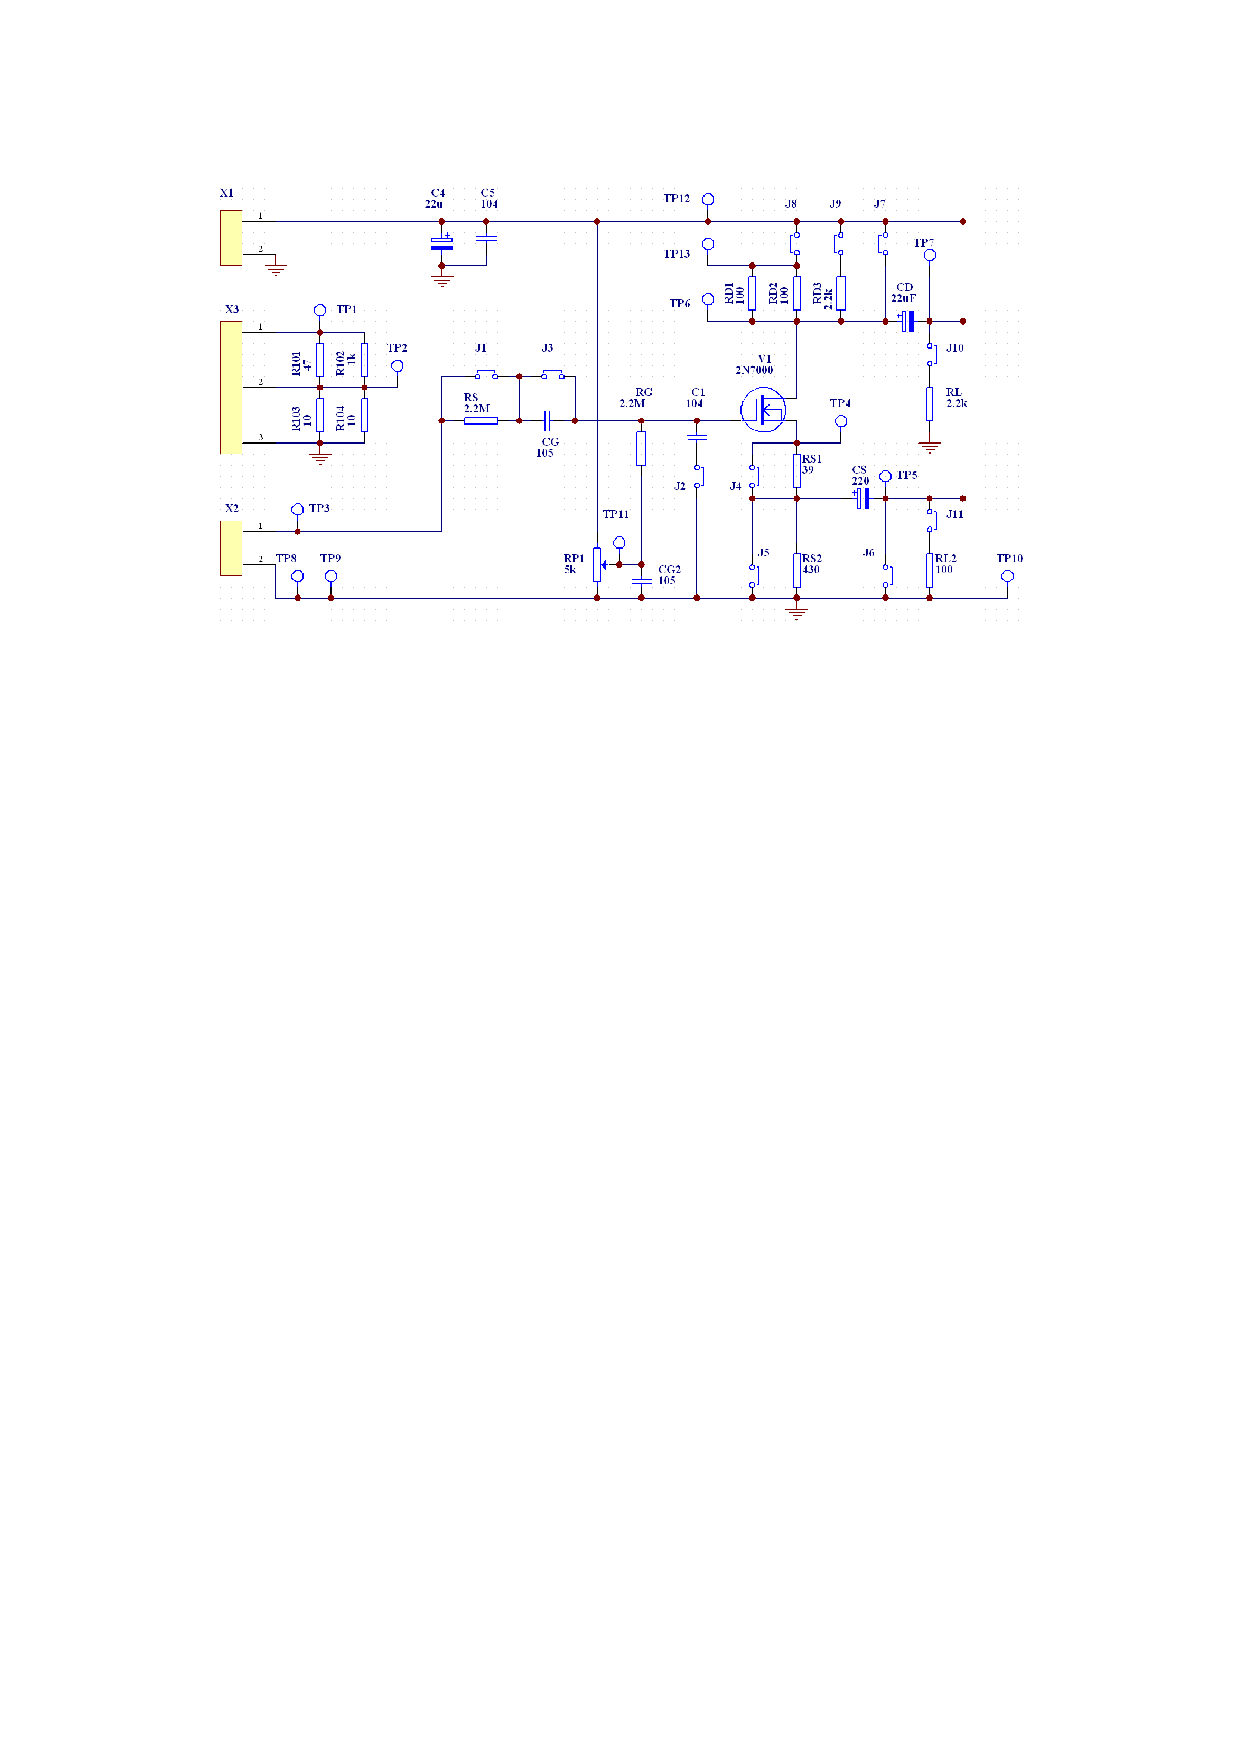
\includegraphics[width=0.9\columnwidth]{LCE-04-场效应管/assets/MOSFET 放大器 PCB 原理图.pdf}
    \caption{MOSFET 放大器 PCB 原理图}
    \label{fig: MOSFET 放大器 PCB 原理图}
\end{figure}

\subsection{测量 MOSFET (2N7000) 特性曲线}

我们并没有按照课件上的方法(逐点法、示波器 XY 轴法)来测量 MOSFET 的特性曲线,而是使用了 Analog Discovery 1 (AD1) 以及 WaveForms 中的 ``Tracer'' 功能来进行测量。这样不仅提高了测量效率,还能将测量数据导出在 MATLAB 中进一步处理,比如计算出 $r_O$, $g_m$、$\frac{g_m}{I_D}$ (transconductance efficiency) 等小信号参数以及 $R_{ON}$ (导通电阻)。

事实上,即使是按照我们的方法来测量,过程也是比较繁琐的,因为我们想测得的数据比课件中要求的多得多。我们希望分别测量 $I_D = 0 \sim 5 \ \mathrm{mA},\ 0 \sim 25 \ \mathrm{mA},\ 0 \sim 125 \ \mathrm{mA}$ 三个电流档位下的特性曲线,能为实际设计提供良好的参考。为节省篇幅,这一部分的具体实验记录放在了我的个人网站,我们就不在此多赘述了,实验记录网址如下:\\ 
% 这里是链接
\href{https://yidingg.github.io/YiDingg/\#/Blogs/Electronics/Transistor\%20Measurement\%20of\%202N7000\%20(N\%20VDMOS)
}{ % 这里是文字
\hspace*{2em} YiDingg's Website > Blogs > Electronics > Transistor Measurement of 2N7000 (N-Channel VDMOS) 
\\ {\color{black}\small \hspace*{2em} https://yidingg.github.io/YiDingg/\#/Blogs/Electronics/Transistor\%20Measurement\%20of\%202N7000\%20(N\%20VDMOS)}
}

将所得输出导出后,进行数据处理、计算、拟合与作图,最终得到结果如下:

\subsubsection{2N7000 (NMOS), 3D, Current Level: High (0 $\sim$ 125 mA)}

\begin{figure}[H]\centering
    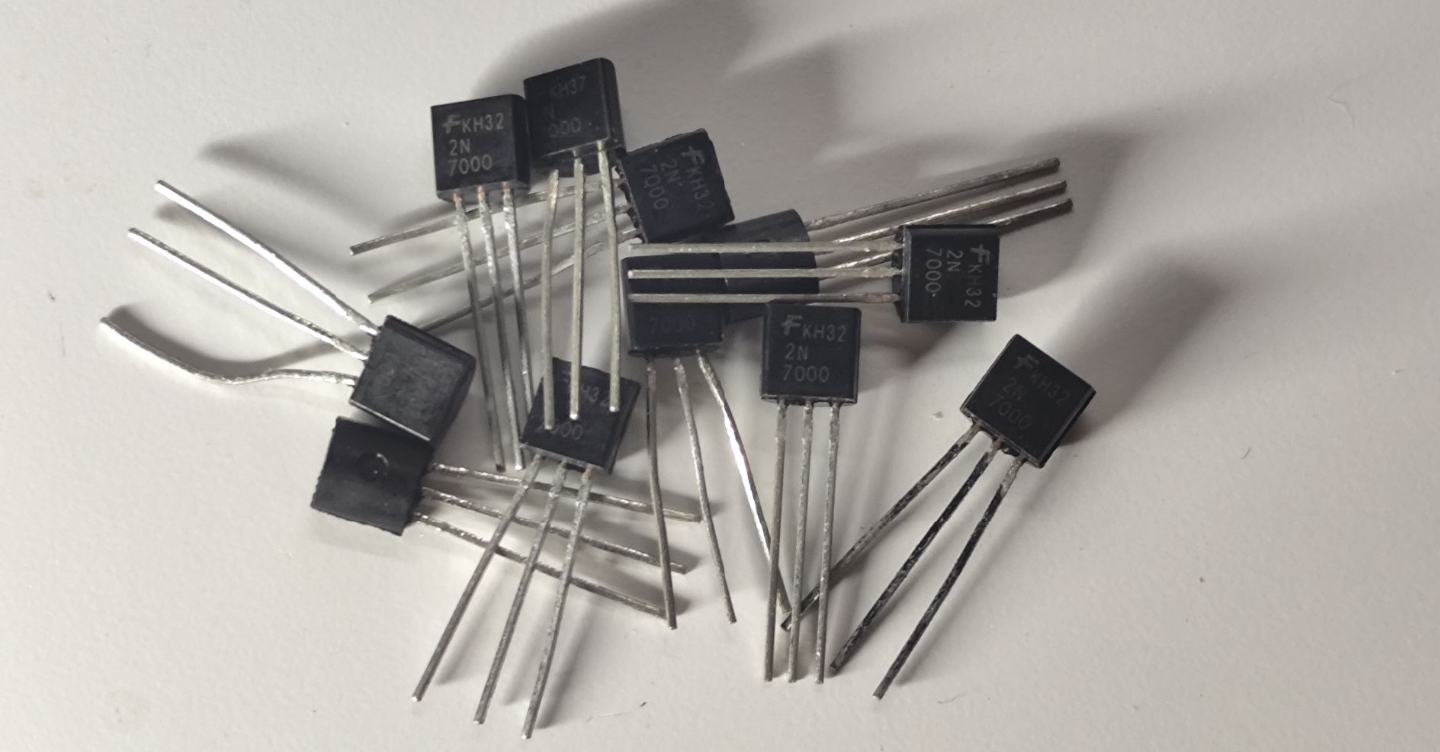
\includegraphics[width=0.6\columnwidth]{LCE-04-场效应管/assets/2N7000/2N7000 (NMOS) [onsemi, KH32] 3D current high/2N7000.png}
    \caption{Product picture}
\end{figure}

\begin{figure}[H]\centering
\begin{subfigure}[b]{0.5\columnwidth}\centering
    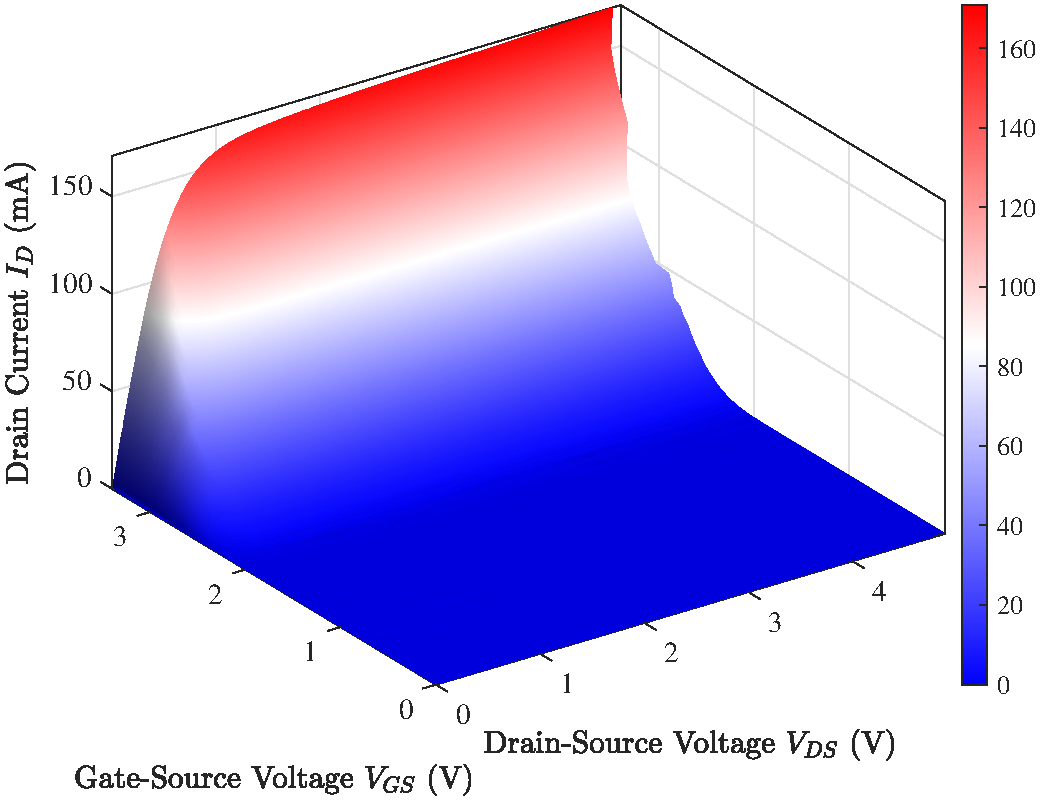
\includegraphics[height=170pt]{LCE-04-场效应管/assets/2N7000/2N7000 (NMOS) [onsemi, KH32] 3D current high/2025-04-24_21-05-11.pdf}
    \caption{Static Characteristics $I_D$ vs. $V_{DS}$}
\end{subfigure}\hfill
\begin{subfigure}[b]{0.5\columnwidth}\centering
    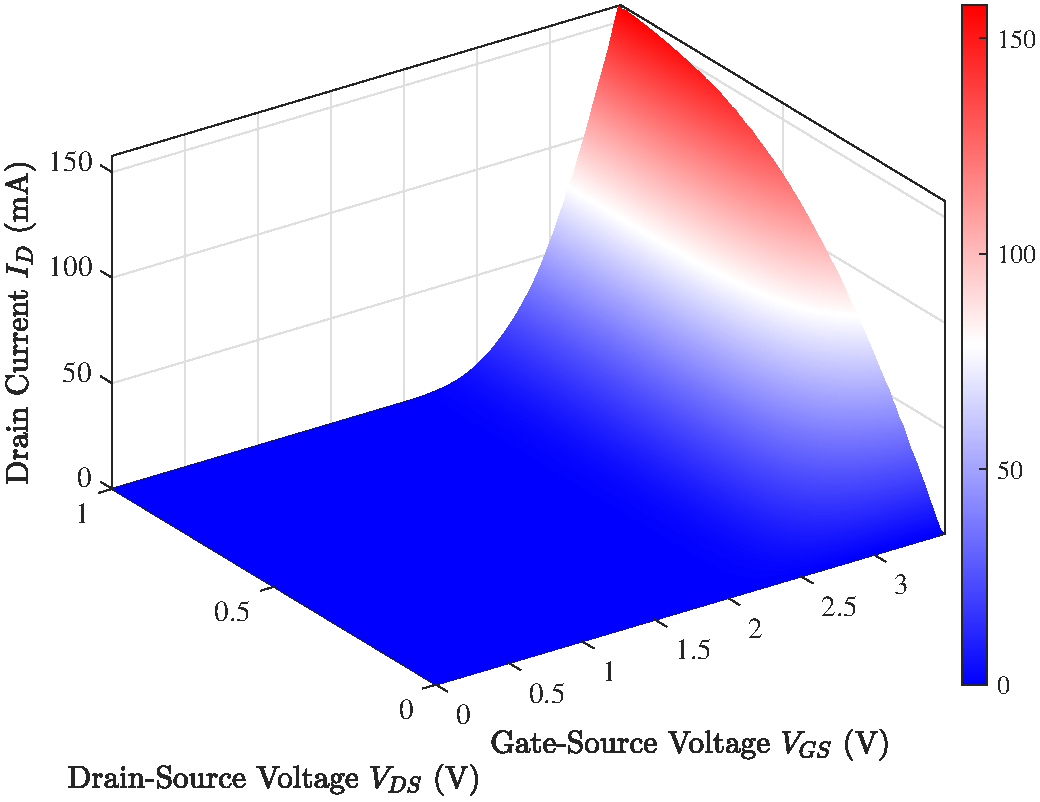
\includegraphics[height=170pt]{LCE-04-场效应管/assets/2N7000/2N7000 (NMOS) [onsemi, KH32] 3D current high/2025-04-24_21-05-16.pdf}
    \caption{Transfer Characteristics $I_D$ vs. $V_{GS}$}
\end{subfigure}
\caption{Characteristics of 2N7000 (3D view)}
\end{figure}


\subsubsection{2N7000 (NMOS), Current Level: Low (0 $\sim$ 5 mA)}

\begin{center}
    \noindent\begin{minipage}{0.45\columnwidth}
        \begin{figure}[H]\centering
            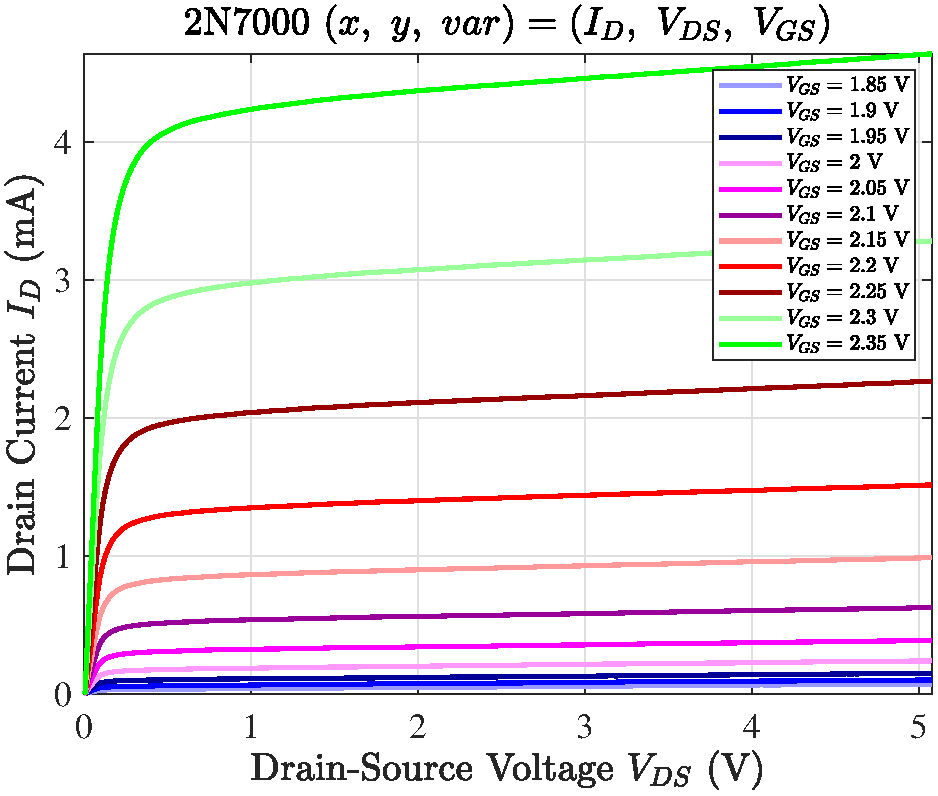
\includegraphics[height=170pt]{LCE-04-场效应管/assets/2N7000/2N7000 (NMOS) [onsemi, KH32] current level low (0~5mA)/2025-04-24_00-33-54__stc_Id_Vds_Vgs.pdf}
            \caption{Static Characteristics $I_D$ vs. $V_{DS}$}
        \end{figure}
        \begin{figure}[H]\centering
            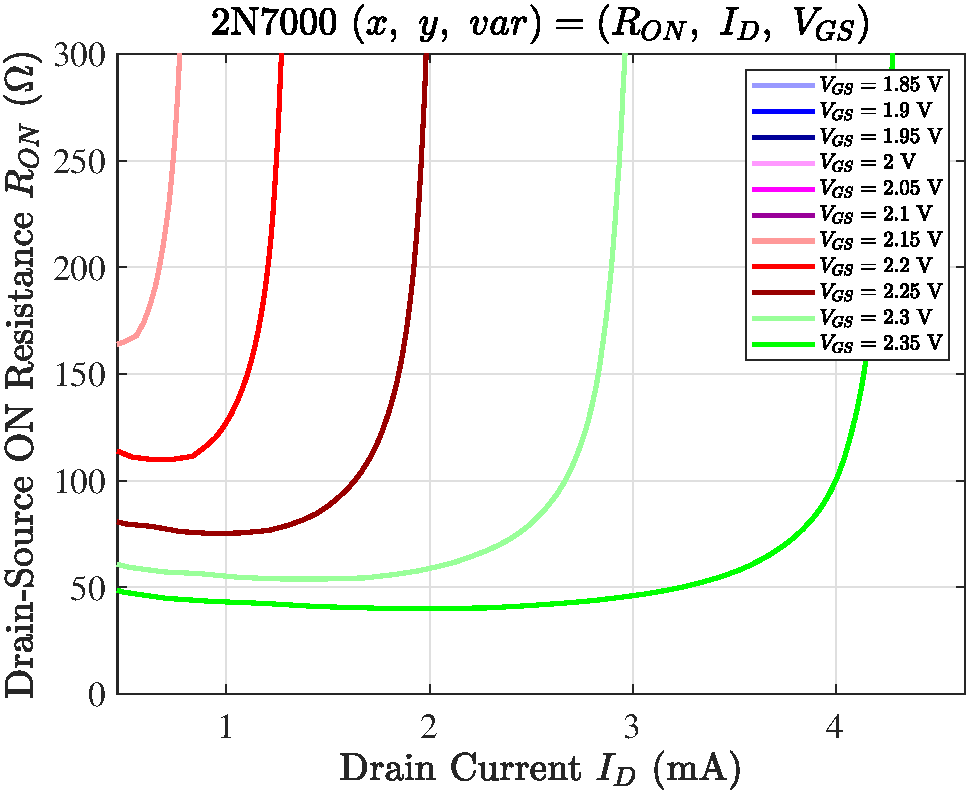
\includegraphics[height=170pt]{LCE-04-场效应管/assets/2N7000/2N7000 (NMOS) [onsemi, KH32] current level low (0~5mA)/2025-04-24_00-33-58__stc_Ron_Id_Vgs.pdf}
            \caption{DS On-Resistance $R_{DS(on)}$ vs. $I_D$}
        \end{figure}
        \begin{figure}[H]\centering
            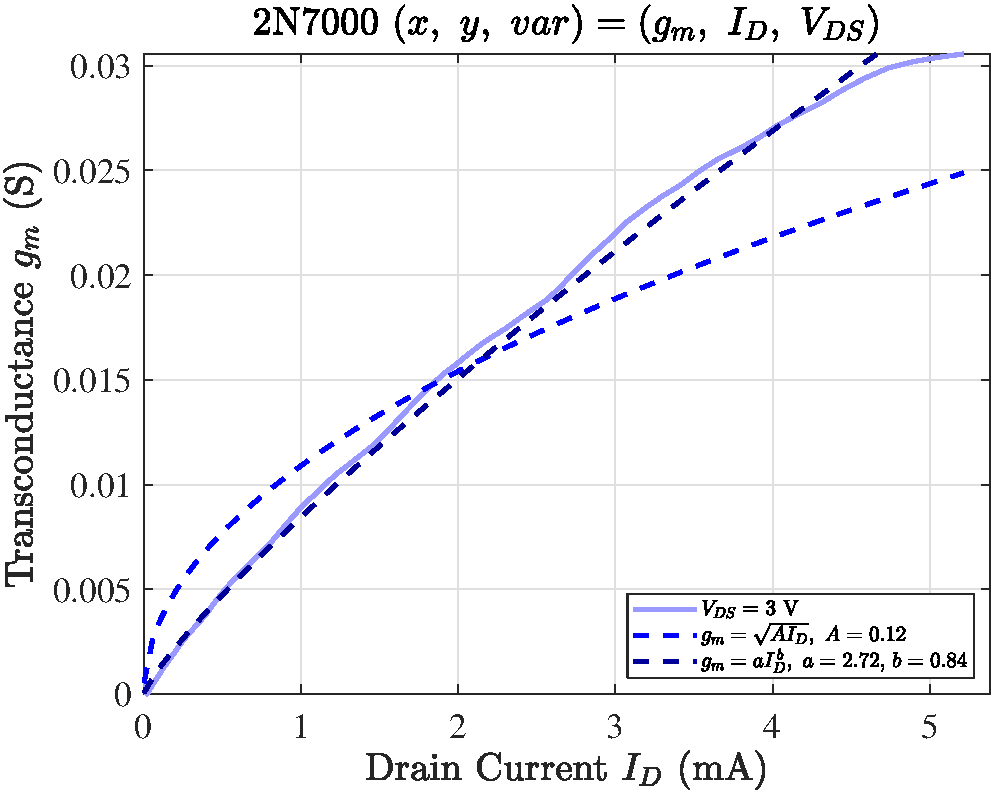
\includegraphics[height=170pt]{LCE-04-场效应管/assets/2N7000/2N7000 (NMOS) [onsemi, KH32] current level low (0~5mA)/2025-04-24_00-34-02__stc_gm_Id_Vds.pdf}
            \caption{Transconductance $g_m$ vs. $I_D$}
        \end{figure}
    \end{minipage}\hfill\begin{minipage}{0.45\columnwidth}
        \begin{figure}[H]\centering
            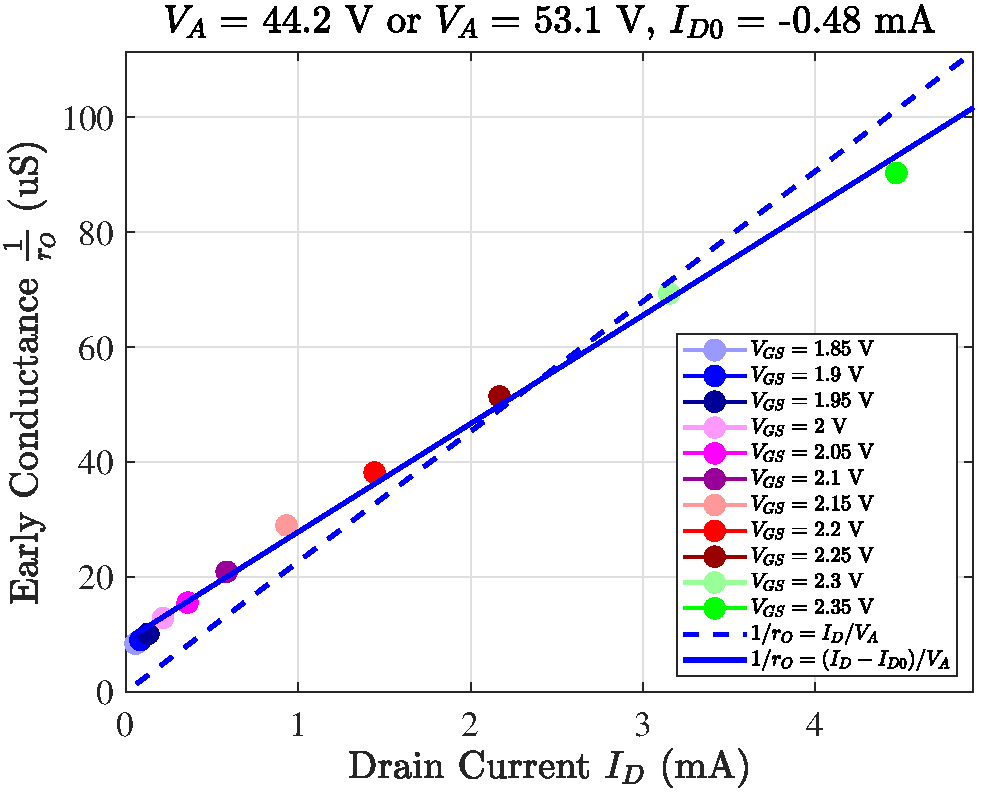
\includegraphics[height=170pt]{LCE-04-场效应管/assets/2N7000/2N7000 (NMOS) [onsemi, KH32] current level low (0~5mA)/2025-04-24_00-33-56__stc_rO_Id_Vgs.pdf}
            \caption{Early Conductance $\frac{1}{r_O}$ vs. $I_D$}
        \end{figure}
        \begin{figure}[H]\centering
            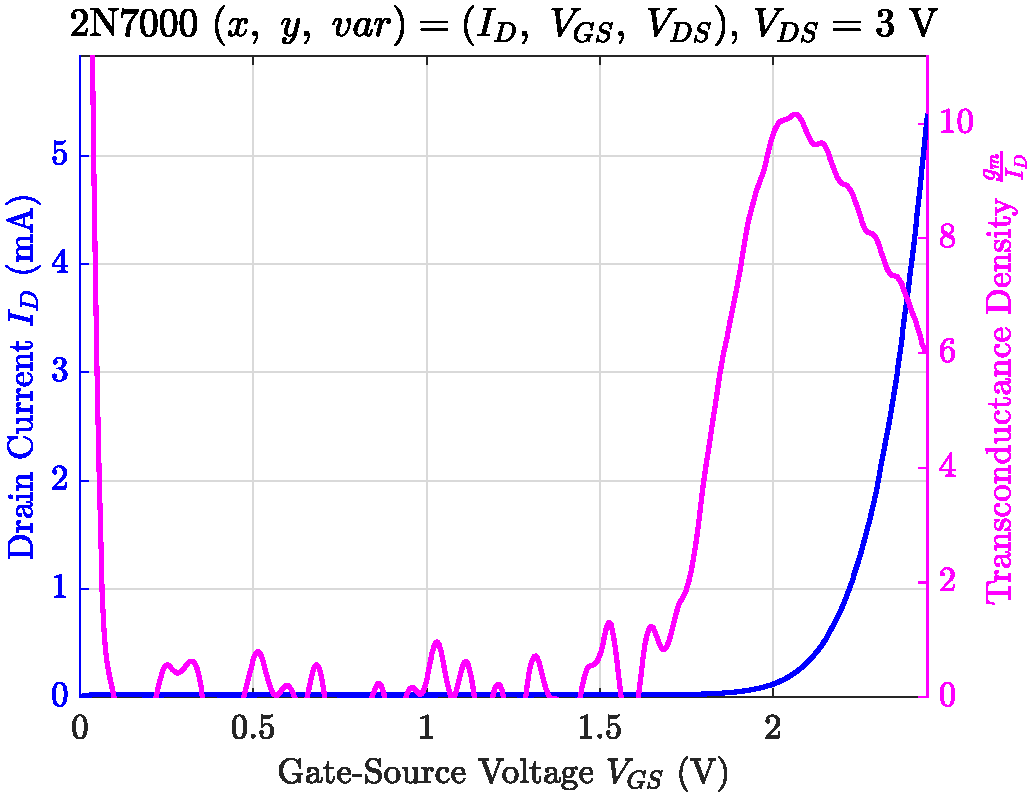
\includegraphics[height=170pt]{LCE-04-场效应管/assets/2N7000/2N7000 (NMOS) [onsemi, KH32] current level low (0~5mA)/2025-04-24_00-34-00__stc_Id_Vgs_Vds.pdf}
            \caption{Transfer Characteristics $I_D$ vs. $V_{GS}$}
        \end{figure}
        \begin{figure}[H]\centering
            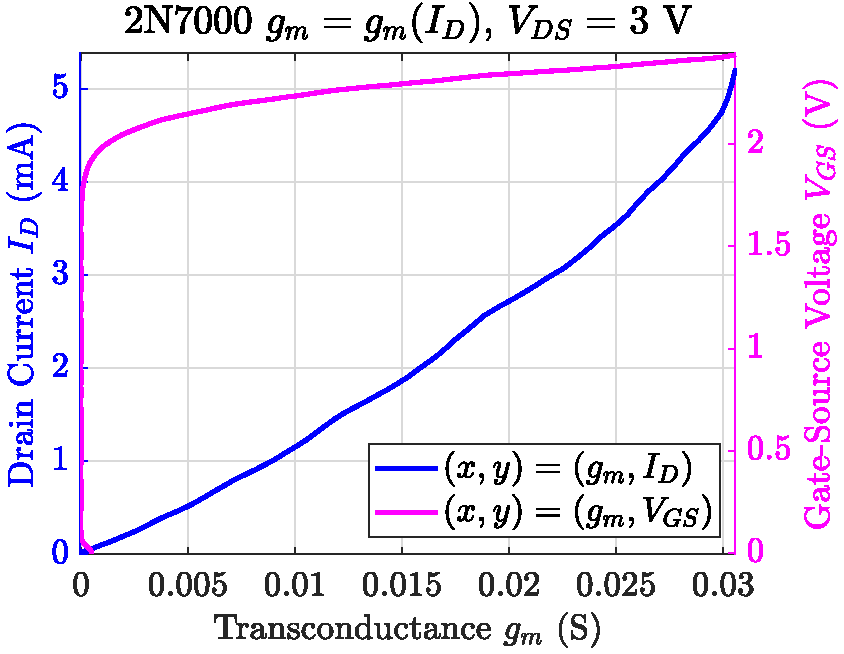
\includegraphics[height=170pt]{LCE-04-场效应管/assets/2N7000/2N7000 (NMOS) [onsemi, KH32] current level low (0~5mA)/2025-04-24_00-34-17__stc_gm_IdVgs_yyplot.pdf}
            \caption{Transconductance $g_m$ vs. $I_D$ and $V_{GS}$}
    \end{figure}
\end{minipage}\end{center}
%LCE-04-场效应管/assets/2N7000/2N7000 (NMOS) [onsemi, KH32] 3D current high/2025-04-24_21-05-16.pdf

\newpage
\subsubsection{2N7000 (NMOS), Current Level: Medium (0 $\sim$ 25 mA)}

\begin{center}
\noindent\begin{minipage}{0.45\columnwidth}
    \begin{figure}[H]\centering
        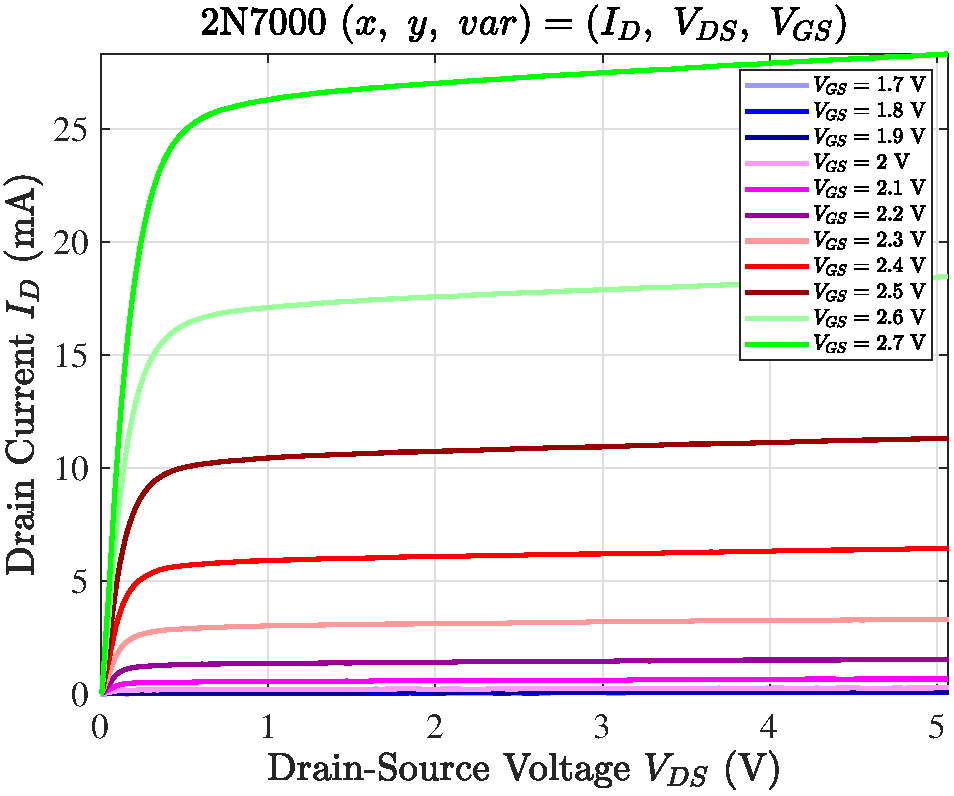
\includegraphics[height=170pt]{LCE-04-场效应管/assets/2N7000/2N7000 (NMOS) [onsemi, KH32] current level mid (0~25mA)/2025-04-24_00-04-22__stc_Id_Vds_Vgs.pdf}
        \caption{Static Characteristics $I_D$ vs. $V_{DS}$}
    \end{figure}
    \begin{figure}[H]\centering
        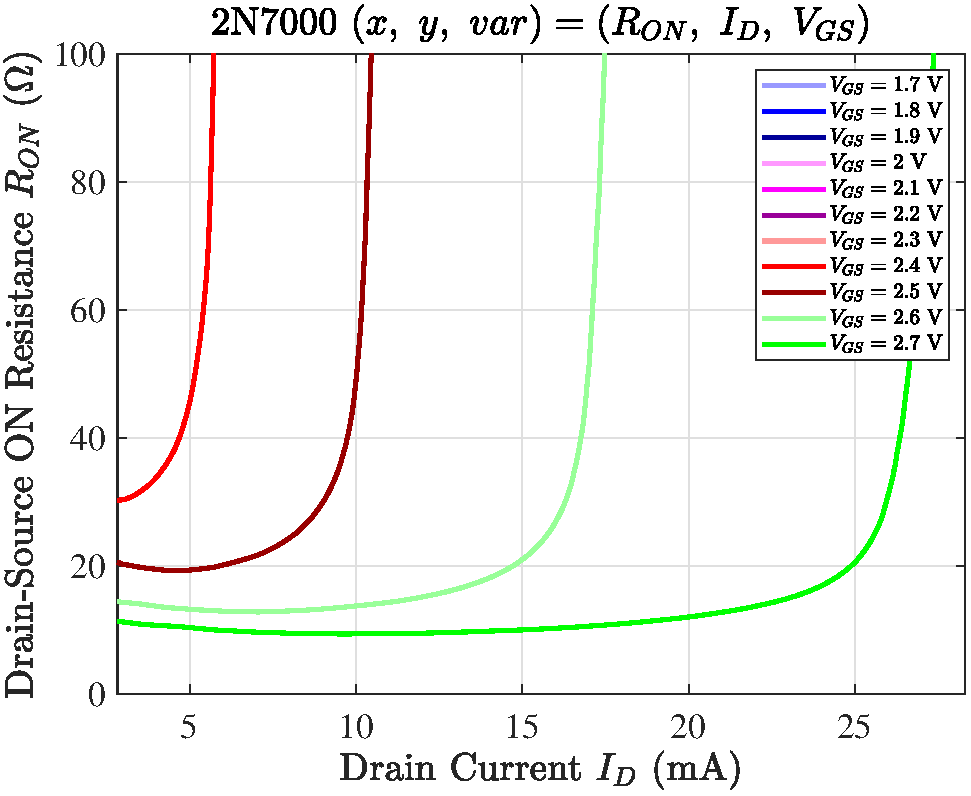
\includegraphics[height=170pt]{LCE-04-场效应管/assets/2N7000/2N7000 (NMOS) [onsemi, KH32] current level mid (0~25mA)/2025-04-24_00-00-07__stc_Ron_Id_Vgs.pdf}
        \caption{DS On-Resistance $R_{DS(on)}$ vs. $I_D$}
    \end{figure}
    \begin{figure}[H]\centering
        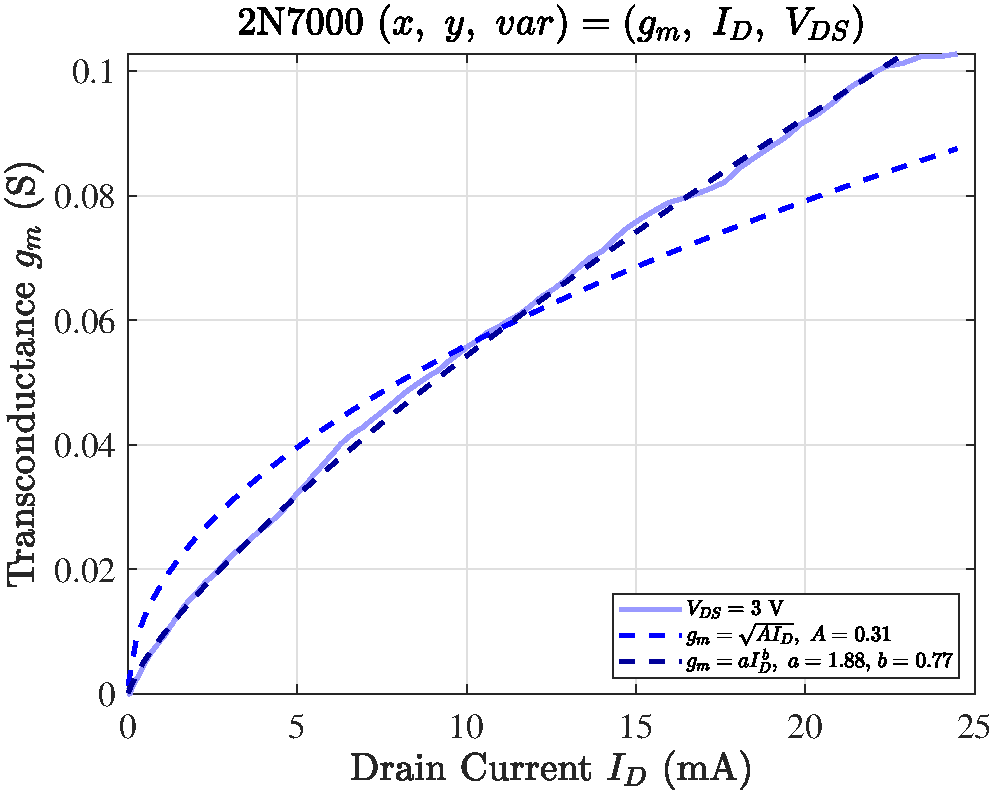
\includegraphics[height=170pt]{LCE-04-场效应管/assets/2N7000/2N7000 (NMOS) [onsemi, KH32] current level mid (0~25mA)/2025-04-24_00-04-29__stc_gm_Id_Vds.pdf}
        \caption{Transconductance $g_m$ vs. $I_D$}
    \end{figure}
\end{minipage}\hfill\begin{minipage}{0.45\columnwidth}
    \begin{figure}[H]\centering
        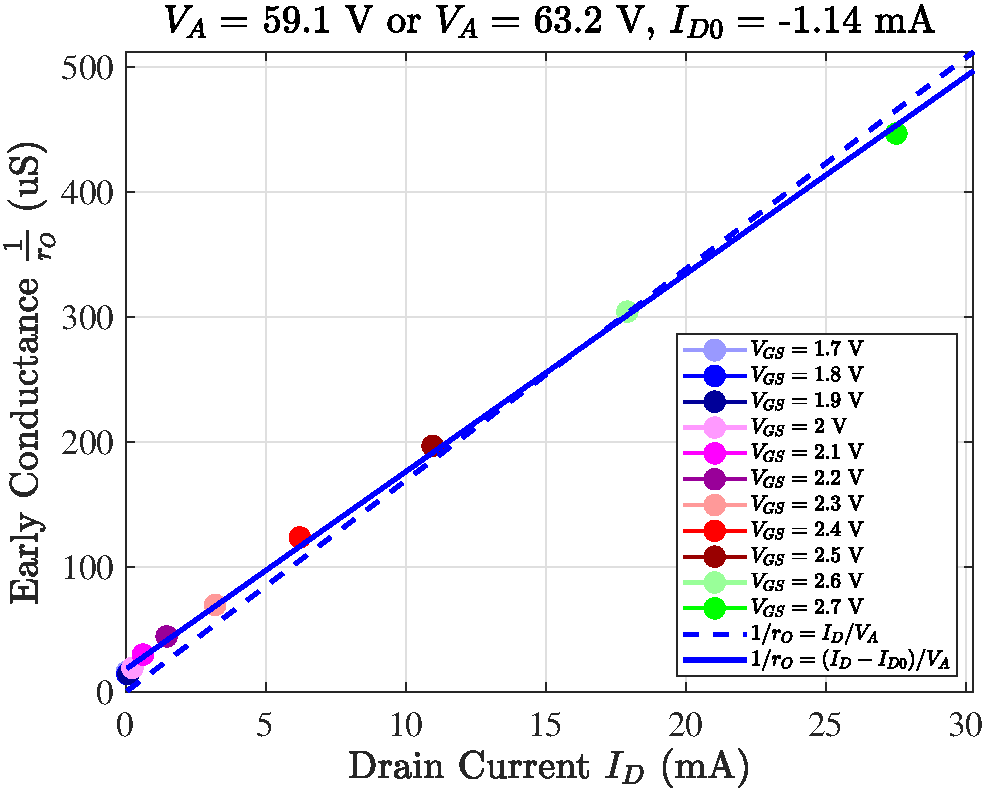
\includegraphics[height=170pt]{LCE-04-场效应管/assets/2N7000/2N7000 (NMOS) [onsemi, KH32] current level mid (0~25mA)/2025-04-24_00-04-24__stc_rO_Id_Vgs.pdf}
        \caption{Early Conductance $\frac{1}{r_O}$ vs. $I_D$}
    \end{figure}
    \begin{figure}[H]\centering
        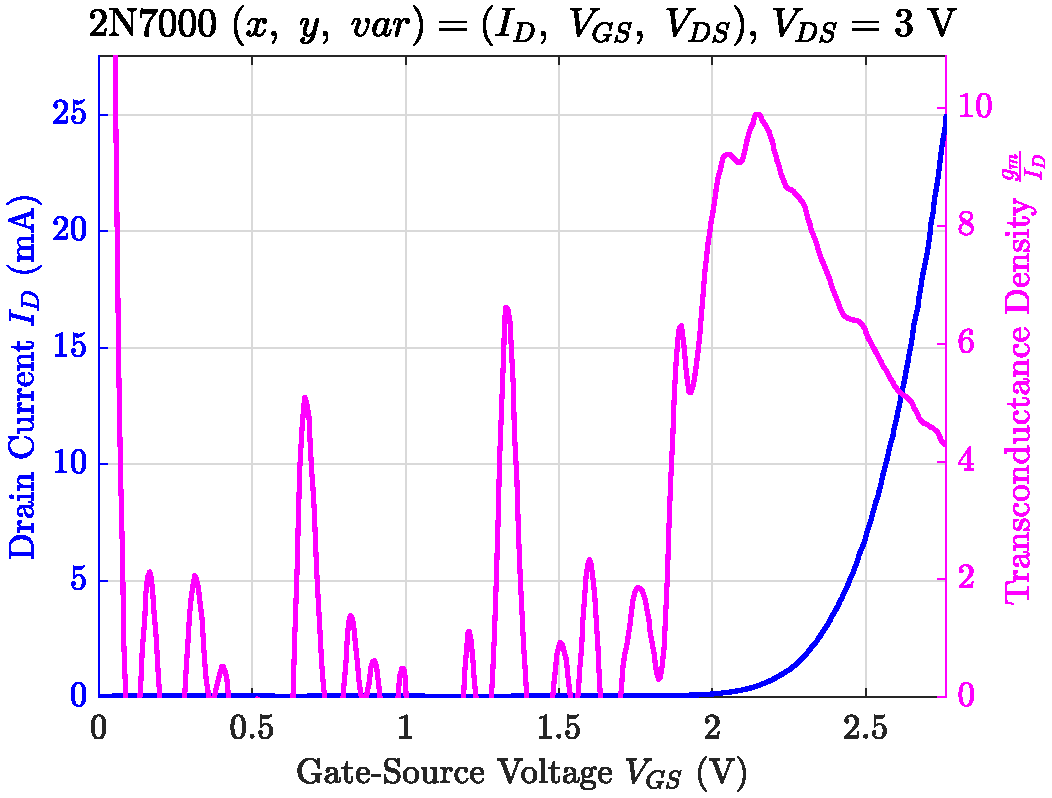
\includegraphics[height=170pt]{LCE-04-场效应管/assets/2N7000/2N7000 (NMOS) [onsemi, KH32] current level mid (0~25mA)/2025-04-24_00-04-28__stc_Id_Vgs_Vds.pdf}
        \caption{Transfer Characteristics $I_D$ vs. $V_{GS}$}
    \end{figure}
    \begin{figure}[H]\centering
        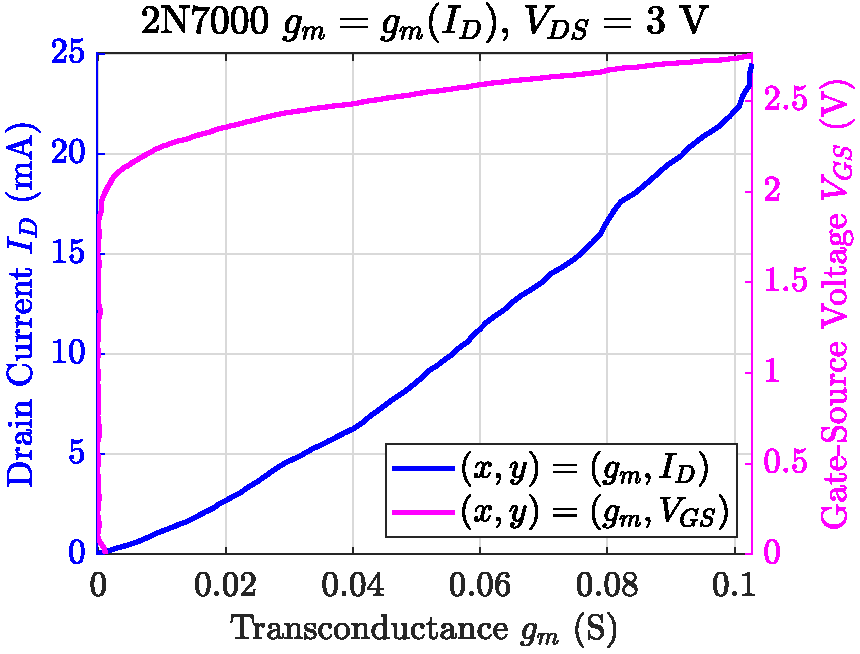
\includegraphics[height=170pt]{LCE-04-场效应管/assets/2N7000/2N7000 (NMOS) [onsemi, KH32] current level mid (0~25mA)/2025-04-24_00-04-31__stc_gm_IdVgs_yyplot.pdf}
        \caption{Transconductance $g_m$ vs. $I_D$ and $V_{GS}$}
    \end{figure}
\end{minipage}\end{center}


\newpage
\subsubsection{2N7000 (NMOS), Current Level: High (0 $\sim$ 125 mA)}


\begin{center}
    \noindent\begin{minipage}{0.45\columnwidth}
        \begin{figure}[H]\centering
            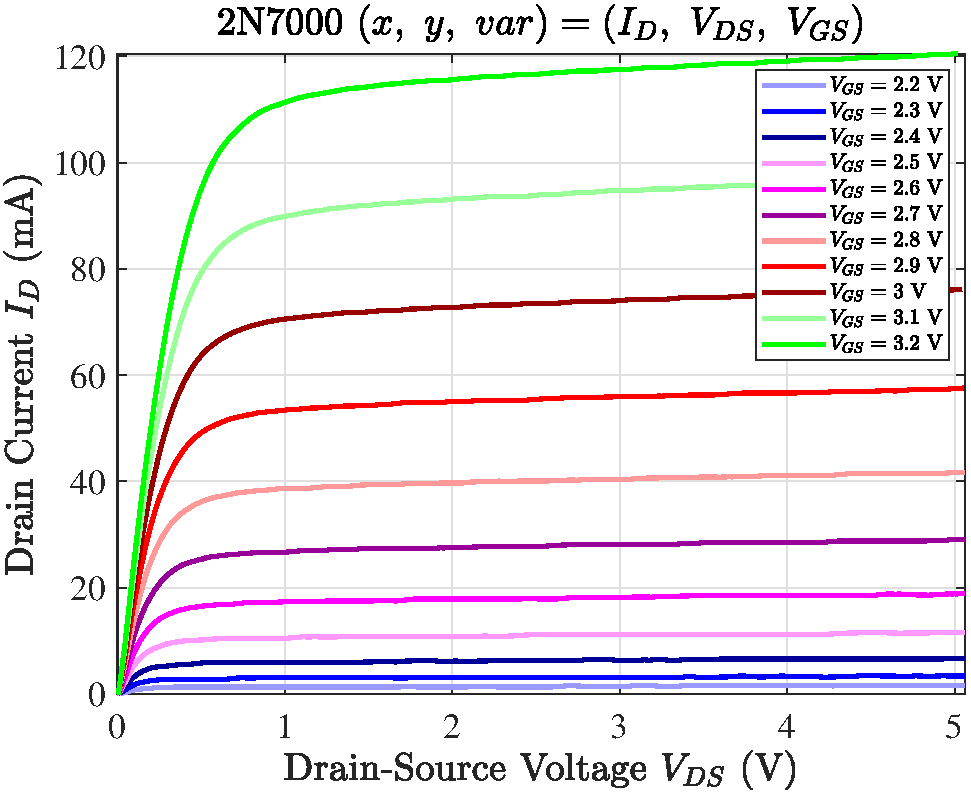
\includegraphics[height=170pt]{LCE-04-场效应管/assets/2N7000/2N7000 (NMOS) [onsemi, KH32] current level high/2025-04-24_00-52-18__stc_Id_Vds_Vgs.pdf}
            \caption{Static Characteristics $I_D$ vs. $V_{DS}$}
        \end{figure}
        \begin{figure}[H]\centering
            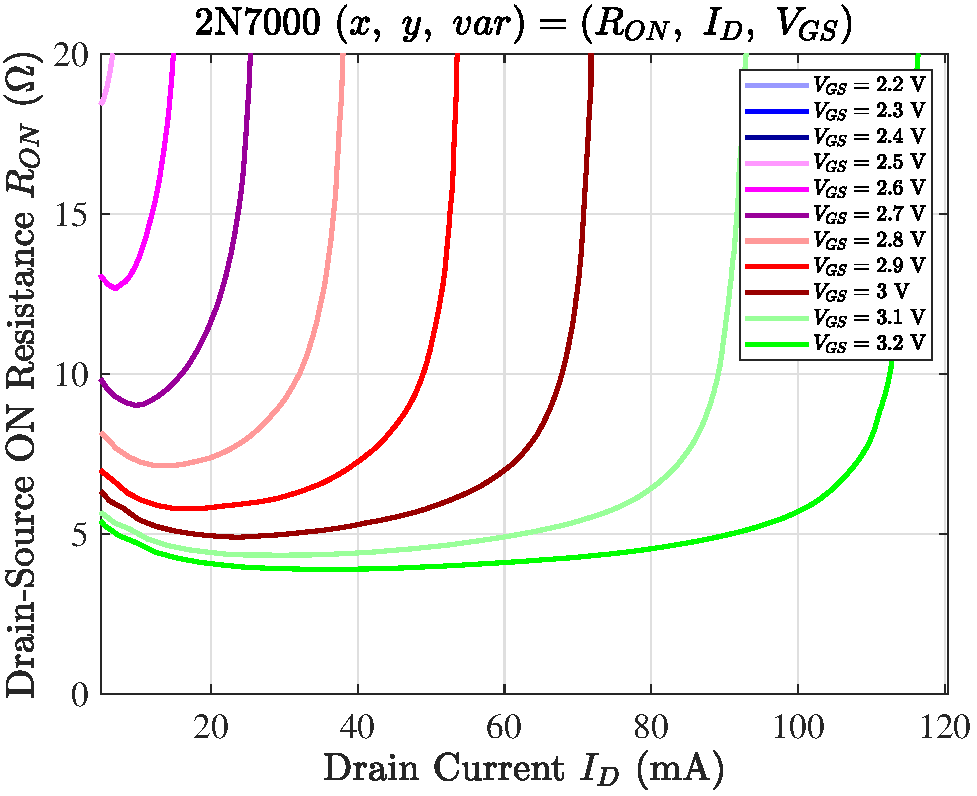
\includegraphics[height=170pt]{LCE-04-场效应管/assets/2N7000/2N7000 (NMOS) [onsemi, KH32] current level high/2025-04-24_00-52-28__stc_Ron_Id_Vgs.pdf}
            \caption{DS On-Resistance $R_{DS(on)}$ vs. $I_D$}
        \end{figure}
        \begin{figure}[H]\centering
            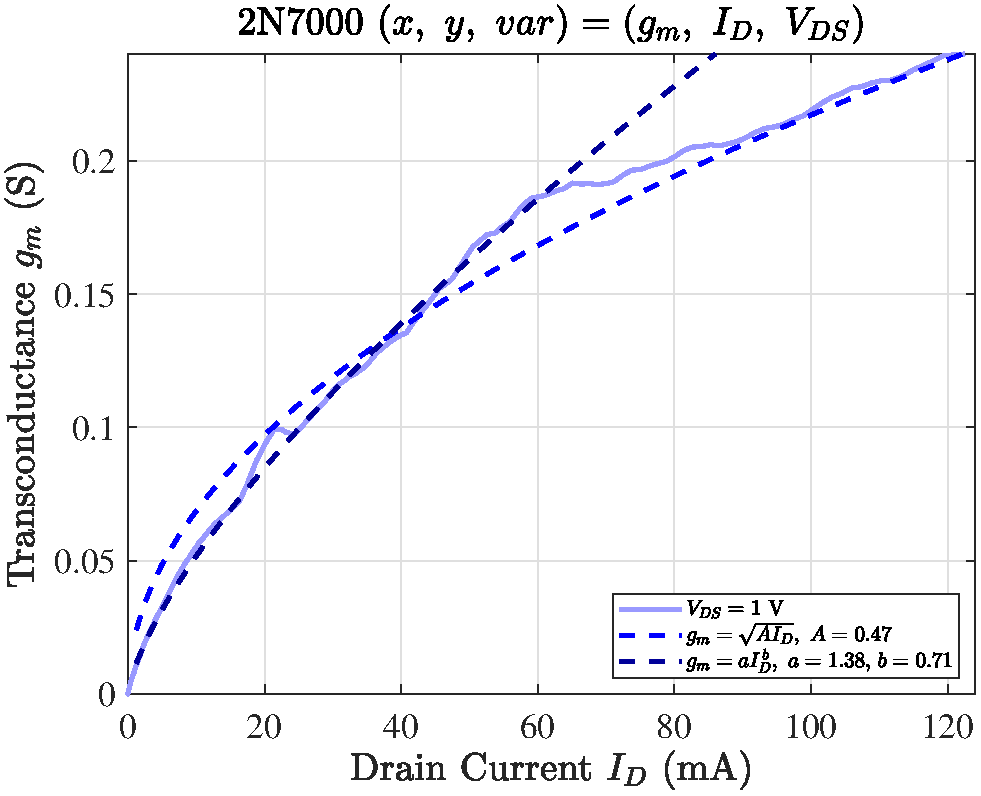
\includegraphics[height=170pt]{LCE-04-场效应管/assets/2N7000/2N7000 (NMOS) [onsemi, KH32] current level high/2025-04-24_00-52-33__stc_gm_Id_Vds.pdf}
            \caption{Transconductance $g_m$ vs. $I_D$}
        \end{figure}
    \end{minipage}\hfill\begin{minipage}{0.45\columnwidth}
        \begin{figure}[H]\centering
            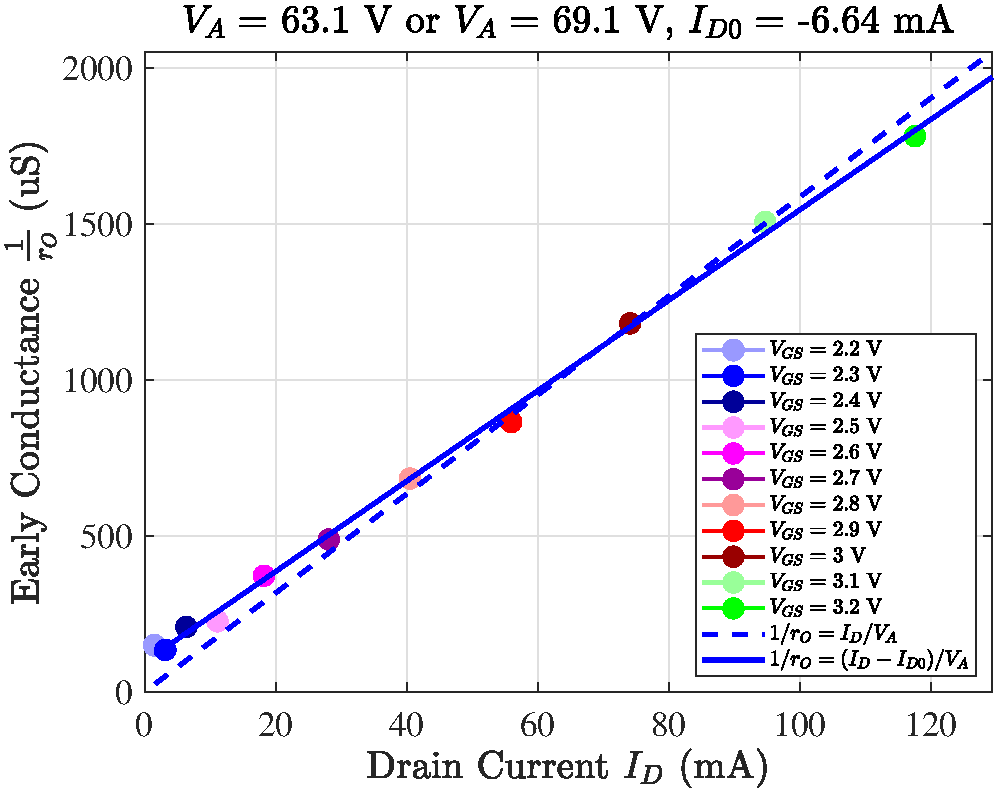
\includegraphics[height=170pt]{LCE-04-场效应管/assets/2N7000/2N7000 (NMOS) [onsemi, KH32] current level high/2025-04-24_00-52-26__stc_rO_Id_Vgs.pdf}
            \caption{Early Conductance $\frac{1}{r_O}$ vs. $I_D$}
        \end{figure}
        \begin{figure}[H]\centering
            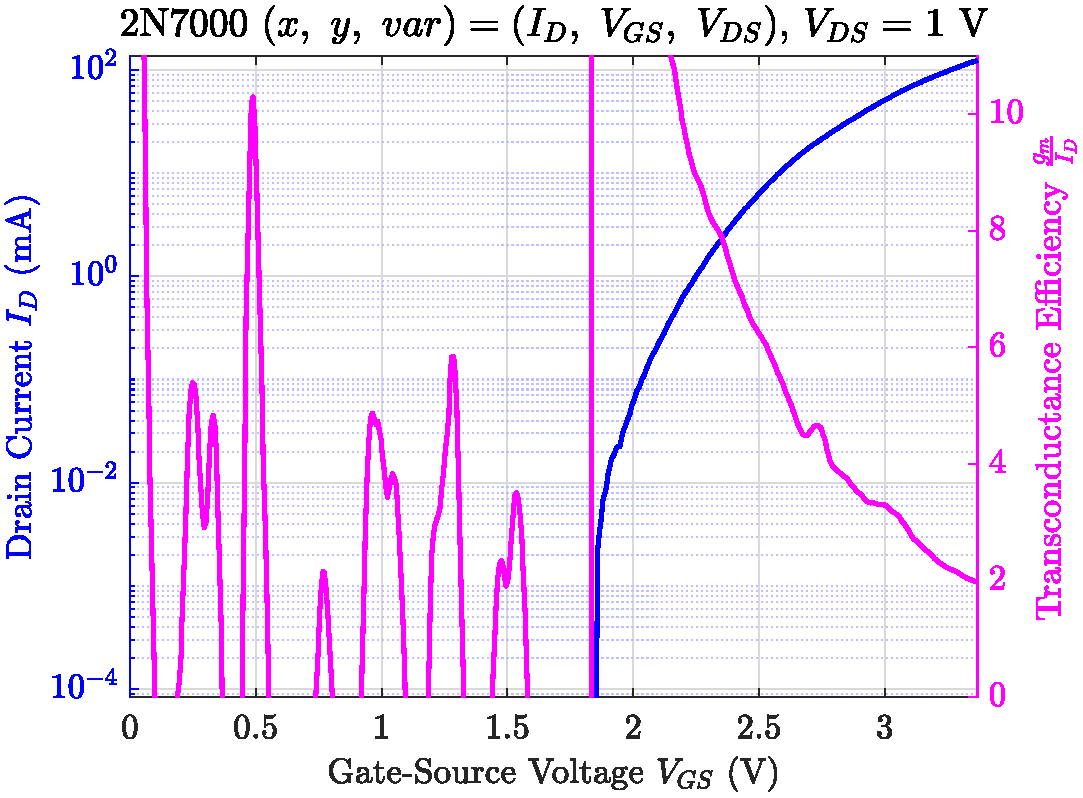
\includegraphics[height=170pt]{LCE-04-场效应管/assets/2N7000/2N7000 (NMOS) [onsemi, KH32] current level high/2025-04-24_00-55-13__stc_Id_Vgs_Vds_logscale.pdf}
            \caption{Transfer Characteristics $I_D$ vs. $V_{GS}$}
        \end{figure}
        \begin{figure}[H]\centering
            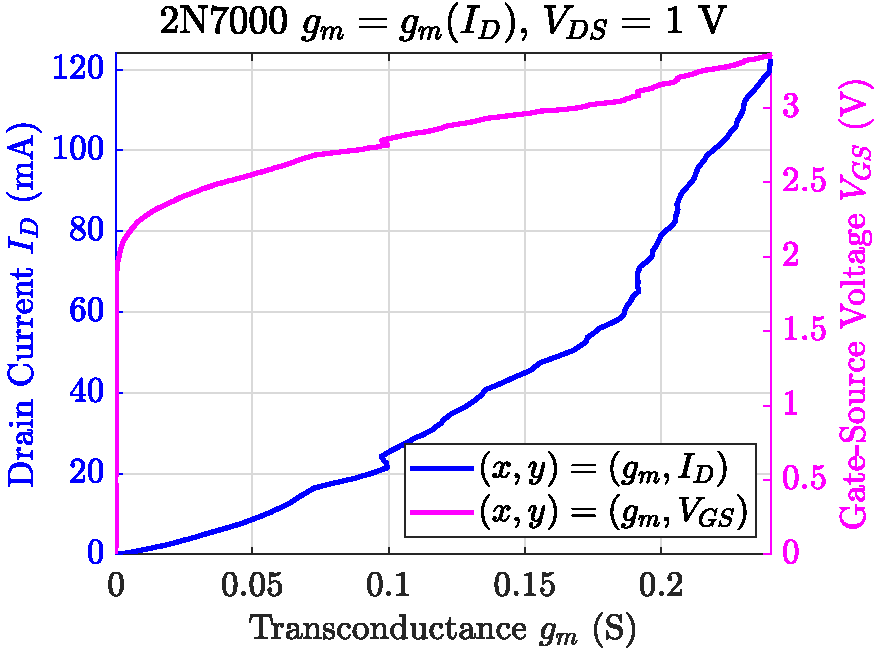
\includegraphics[height=170pt]{LCE-04-场效应管/assets/2N7000/2N7000 (NMOS) [onsemi, KH32] current level high/2025-04-24_00-52-35__stc_gm_IdVgs_yyplot.pdf}
            \caption{Transconductance $g_m$ vs. $I_D$ and $V_{GS}$}
    \end{figure}
\end{minipage}\end{center}








\newpage
\subsection{Common-Source Amplifier}
\vspace*{-3mm}
\begin{redbox}
    若无特别说明,后续实验均默认示波器为 ac coupling 模式,且不扫频时输入信号为 1 kHz sine wave 。
\end{redbox}

\subsubsection{设置静态工作点}

闭合图 \ref{fig: MOSFET 放大器 PCB 原理图} 中的跳线 J1, J5, J9 构成 common-source amplifier ,设置 $V_{CC}$ 为 12 V, 调整电位器使 $V_{GS}$ 在 2.1 V 左右,并且 $R_D = 2.2\ \mathrm{k}\Omega$ 上的压降为 $V_{R_D} = 6.6 \ \mathrm{V}$ (对应 $I_D = 3 \ \mathrm{mA}$),便完成了静态工作点的设置。此时晶体管的工作环境为:
\begin{gather}
I_D = 3 \ \mathrm{mA},\quad R_D = 2.2 \ \mathrm{k}\Omega, \ R_{SS} = 39 \ \Omega
\end{gather}
我们实际调试到了 $V_{GS} = 2.0093 \ \mathrm{V},\  V_{R_D} = 6.598 \ \mathrm{V}$,然后便可进行下面的测量。

\subsubsection{测量频率响应 (原始增益曲线)}

AD1 的 W1 接 TP3, 通过电容 $C_G$ 将信号输入到 MOSFET 的 gate, AD1 的 CH1 和 CH2 分别接在 TP3 和 TP6 (2N7000 的 drain 节点) 处,测量输入信号和输出信号,此时得到的曲线即为空载时的频率响应。设置信号源信号幅度为 100 mVamp (200 mVpp),分别用普源示波器 (用 ``RIGOL'' 表示) 和 AD1 测量输入输出波形,得到结果如下:

\begin{figure}[H]\centering
    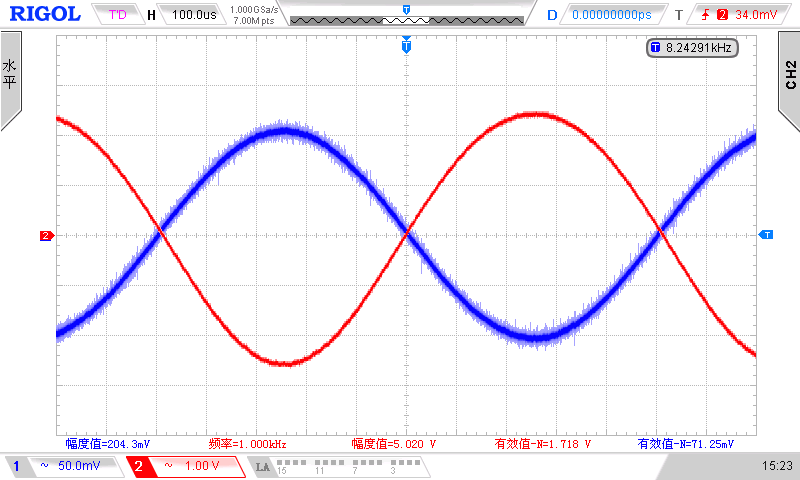
\includegraphics[width=\columnwidth]{LCE-04-场效应管/assets/cs amp/CS 输入输出波形 RIGOL.png}
    \caption{(RIGOL) cs amp. I/O waveform: input (CH1-blue, 100 mVamp @ 1 kHz), output (CH2-red), overlap display}
\end{figure}

\begin{figure}[H]\centering
    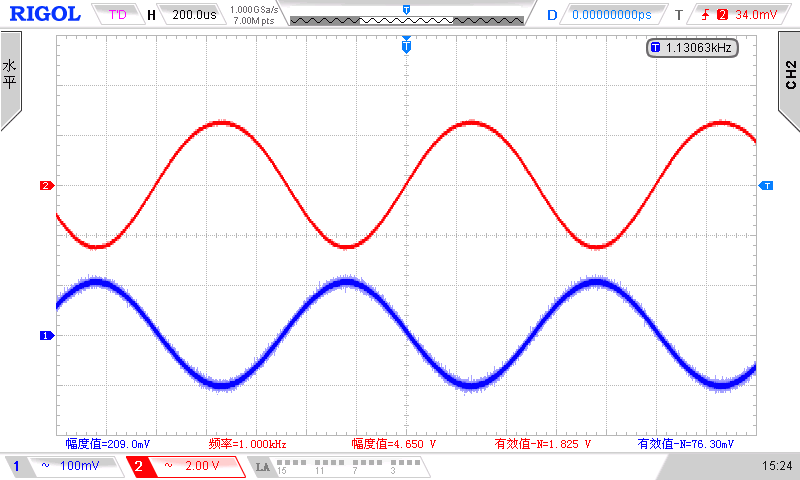
\includegraphics[width=\columnwidth]{LCE-04-场效应管/assets/cs amp/CS 输入输出波形 RIGOL (2).png}
    \caption{(RIGOL) cs amp. I/O waveform: input (CH1-blue, 100 mVamp @ 1 kHz), output (CH2-red), misaligned display}
\end{figure}

\begin{figure}[H]\centering
    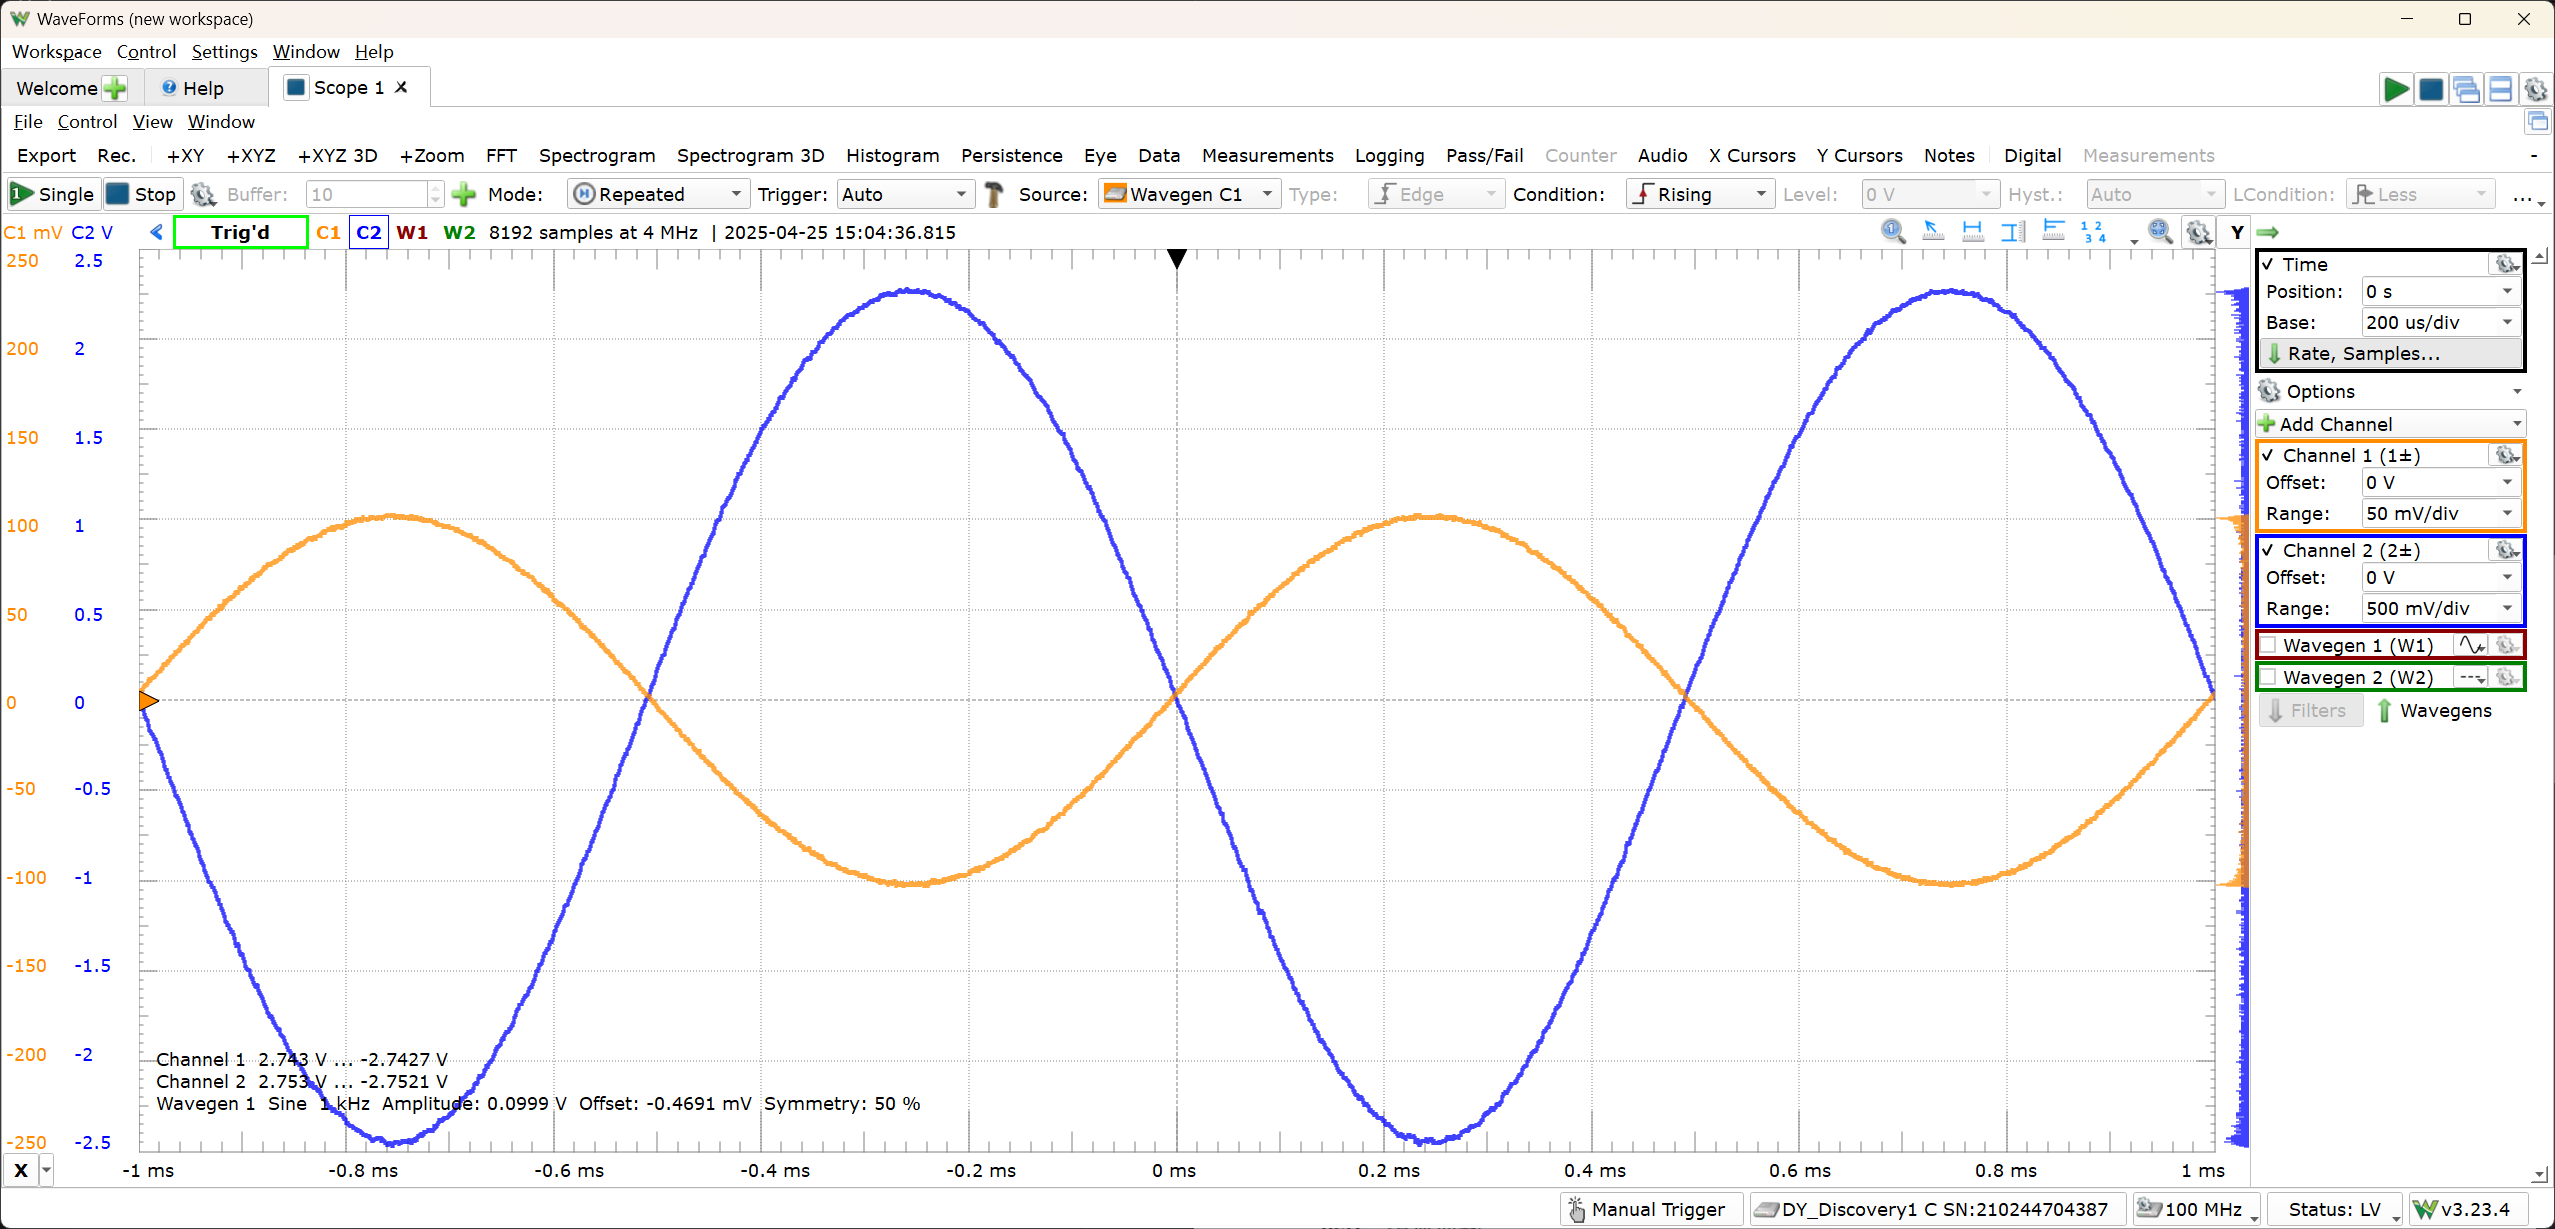
\includegraphics[width=\columnwidth]{LCE-04-场效应管/assets/cs amp/CS 输入输出波形.png}
    \caption{(AD1) cs amp. I/O waveform: input (CH1-orange, 100 mVamp @ 1 kHz), output (CH2-blue), overlap display}
\end{figure}

\begin{figure}[H]\centering
    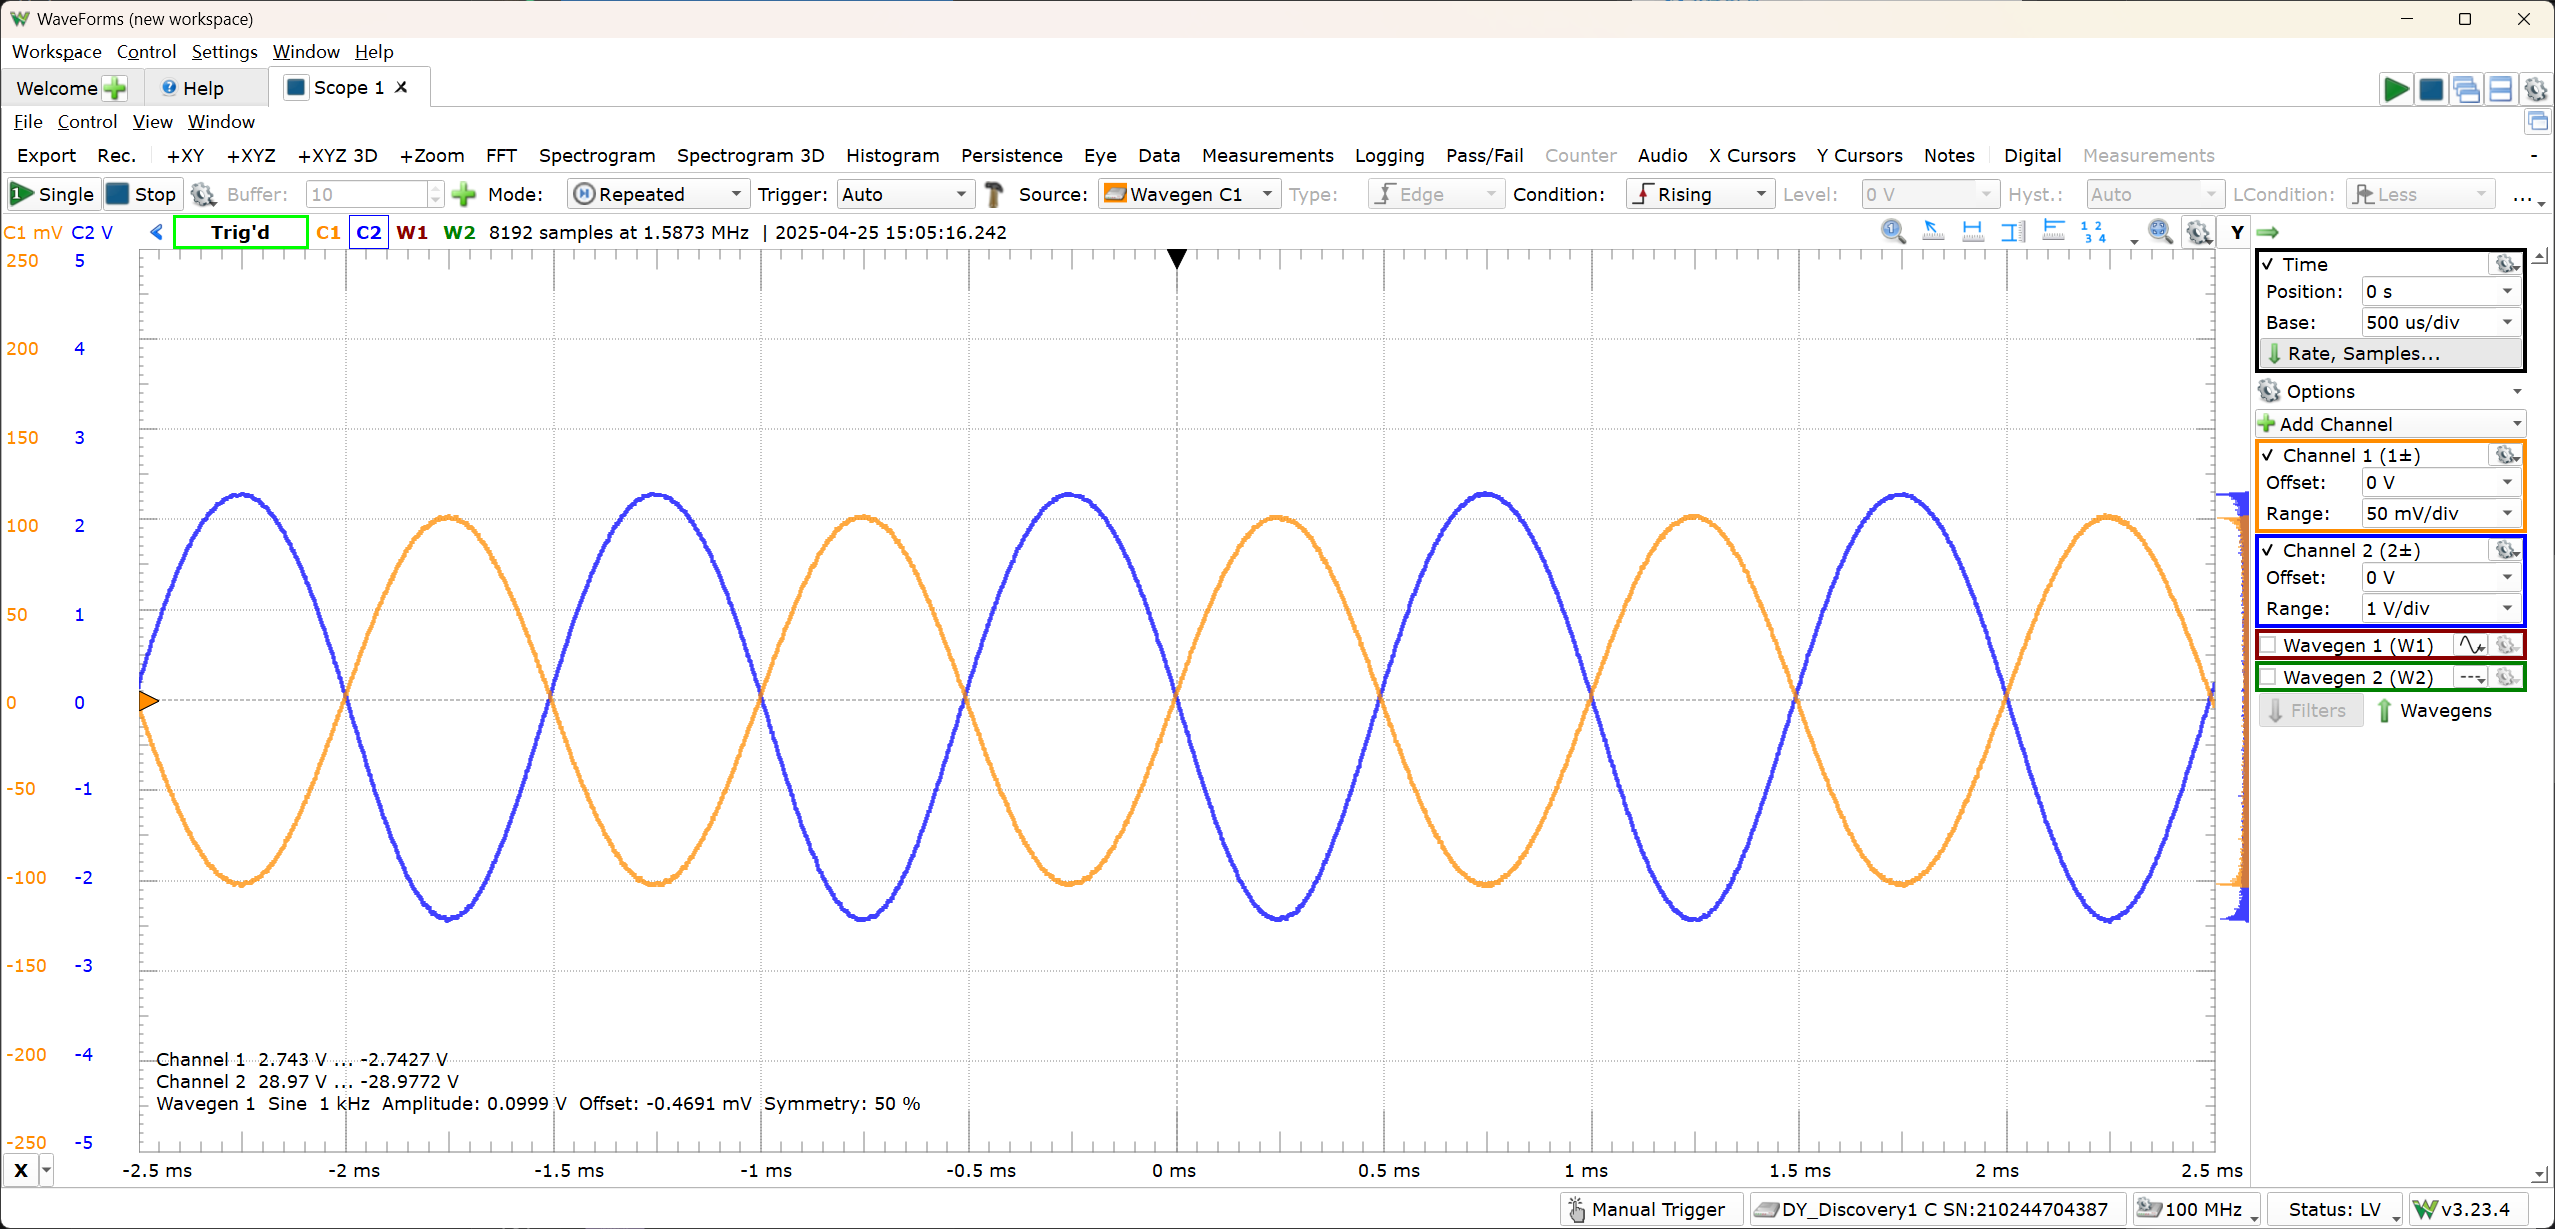
\includegraphics[width=\columnwidth]{LCE-04-场效应管/assets/cs amp/CS 输入输出波形 (2).png}
    \caption{(AD1) cs amp. I/O waveform: input (CH1-orange, 100 mVamp @ 1 kHz), output (CH2-blue), misaligned display}
\end{figure}



\noindent 
保持输入信号不变,进行扫频,得到空载增益曲线 $A_1 = A_1 (f)$ 如图:
\begin{figure}[H]\centering
    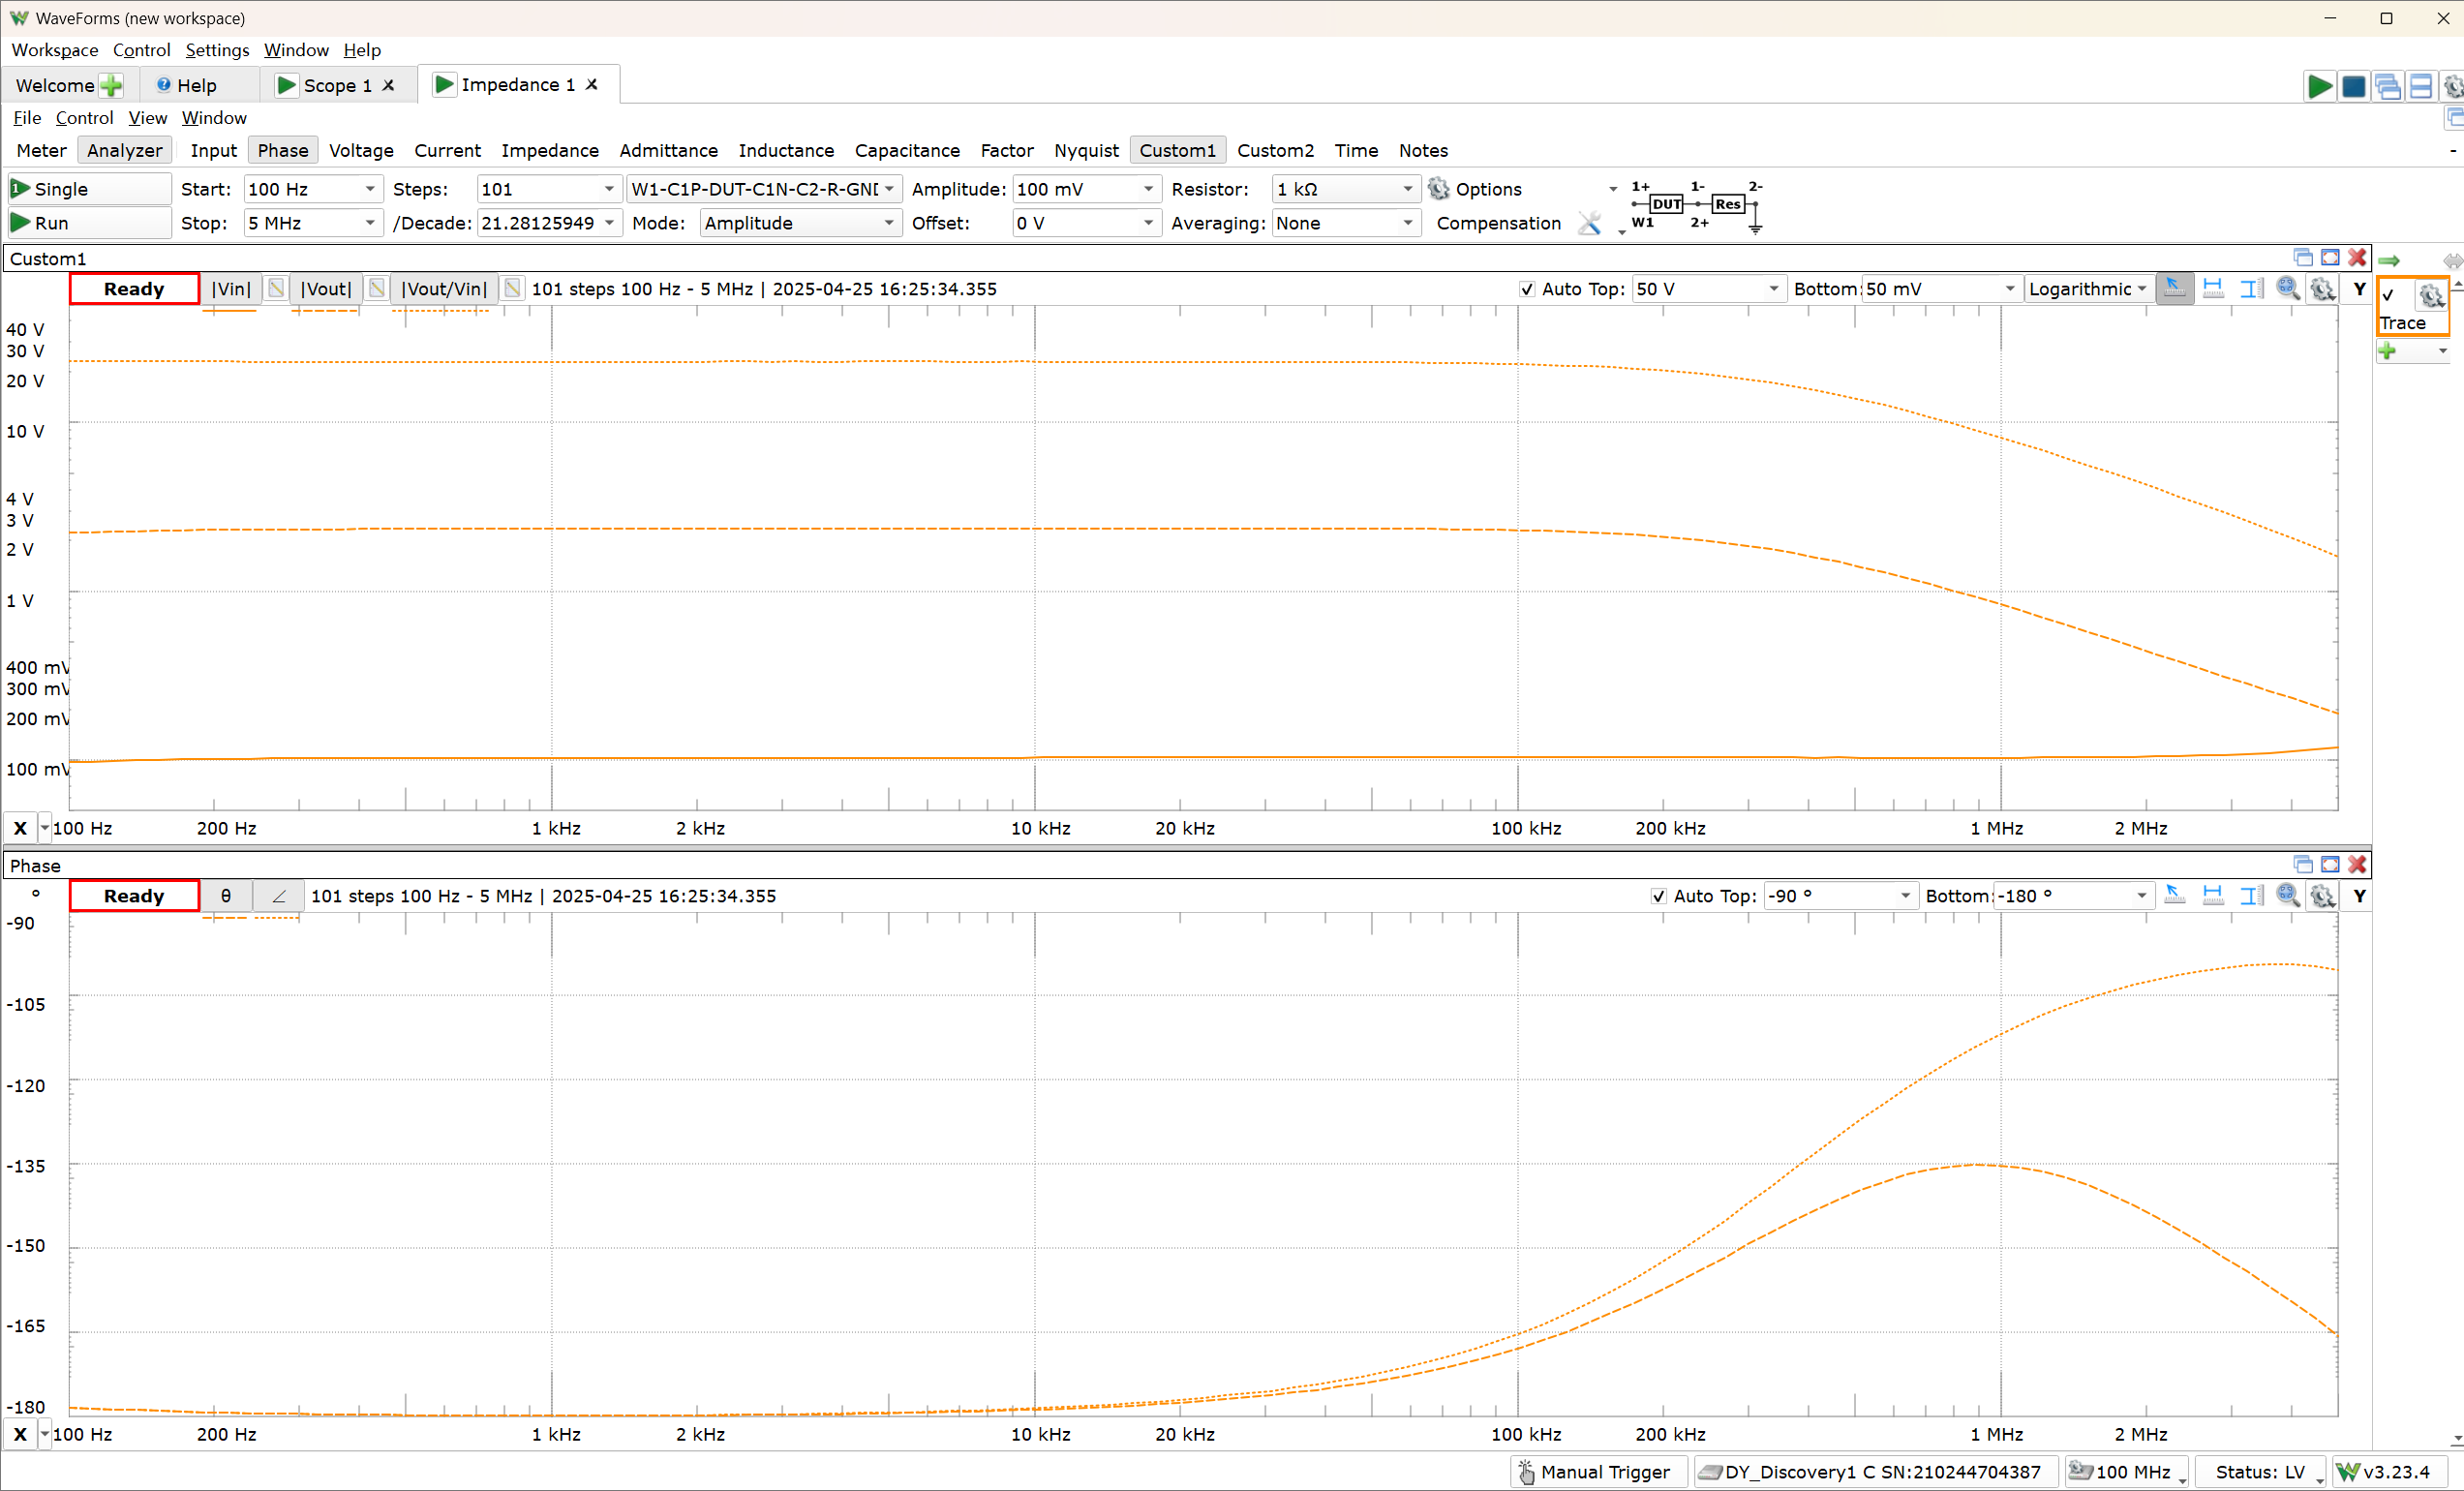
\includegraphics[width=\columnwidth]{LCE-04-场效应管/assets/cs amp/cs amp frequency response (input 100 mVamp, 100Hz ~ 5MHz).png}
    \caption{Common-source amplifier: frequency response (input 100 mVamp from 100 Hz to 5 MHz), $Z_L = \infty,\ R_S = 0$}
\end{figure}
图中的上半部分是输入输出信号与增益曲线,其中 $V_{in,amp}$ 由实线画出,$V_{out,amp}$ 由虚线画出,$|A_v| = \frac{V_{out,amp}}{V_{in,amp}}$ 由更细碎的虚线画出;下半部分是相位曲线,第一条虚线表示的是输出信号相对于 AD1 内部时钟的相位 (无需关心这条曲线),第二条线(细碎虚线)表示的是 $A_v = \frac{V_{out}}{V_{in}}$ 的相位,也即频响曲线中的 phase 。

测量完成后,将数据导出备用,在后文统一进行数据处理。

\subsubsection{测量输出有负载时的增益}

在上一步的基础上,再闭合跳线 J10 (引入负载 $22 \ \mathrm{uF} + 2.2 \ \mathrm{k}\Omega$)。与上面的操作类似,保持输入信号幅度为 100 mVamp 不变,仍在 TP6 (drain 节点) 进行测量,得到带有负载 ($22 \ \mathrm{uF} + 2.2 \ \mathrm{k}\Omega$) 时的频率响应 $A_2 = A_2 (f)$,结果如下图所示:

\begin{figure}[H]\centering
    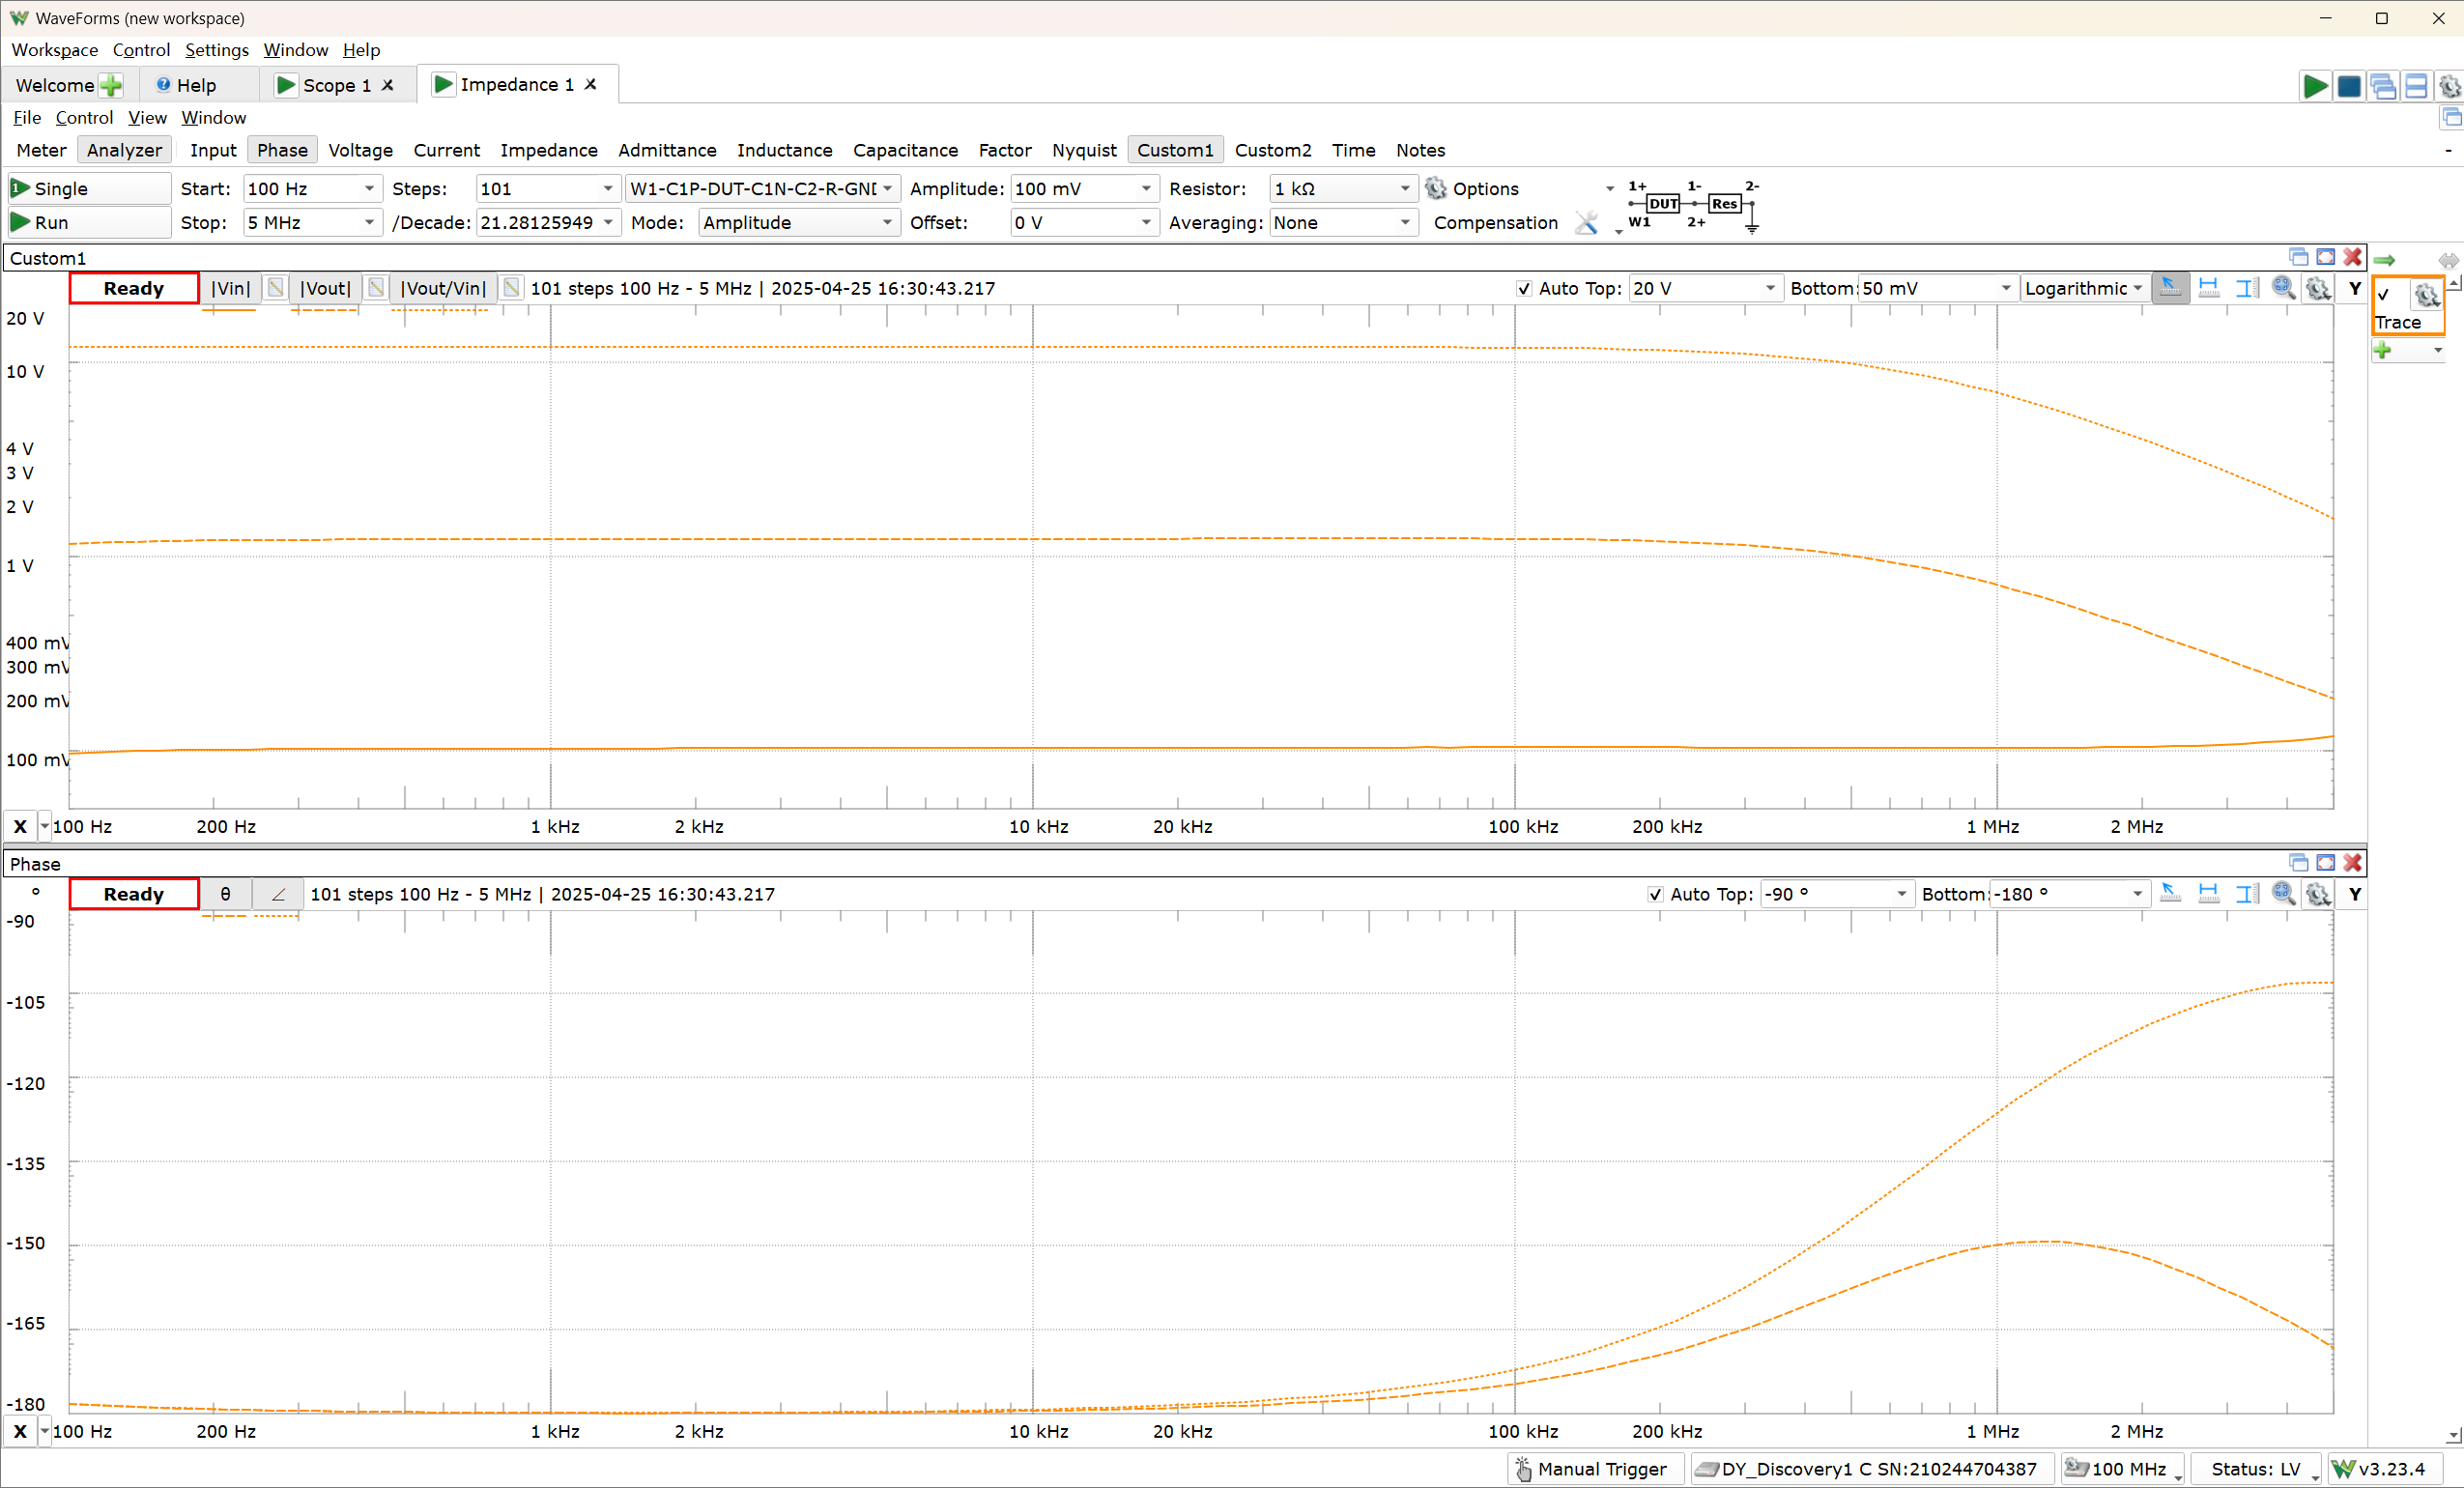
\includegraphics[width=\columnwidth]{LCE-04-场效应管/assets/cs amp/cs amp output impedance, R_L = 2k2 Ohm (input 100 mVamp, 100Hz ~ 5MHz).png}
    \caption{Common-source amp. frequency response: input 100 mVamp from 100 Hz to 5 MHz, $Z_L = 22 \ \mathrm{uF} + 2.2 \ \mathrm{k}\Omega,\ R_S = 0$}
\end{figure}

依据原增益 $A_1$ 和带载增益 $A_2$,可以计算出等效输出阻抗 $Z_{out}$:
\begin{gather}
\label{eq: Z_out}
A_2 = A_1 \cdot \frac{R_L + \frac{1}{sC_{out}}}{R_L + \frac{1}{sC_{out}} + Z_{out}} \Longrightarrow 
Z_{out} = \left(\frac{A_1}{A_2} - 1\right)\cdot \left(R_L + \frac{1}{sC_{out}}\right) = \left(\frac{A_1}{A_2} - 1\right)\cdot \left(R_L + \frac{1}{j\omega C_{out}}\right)
\end{gather}
其中 $R_L = 2.2\mathrm{k}\Omega,\ C_{out} = 22 \ \mathrm{uF}$,注意上式中的 $A_1$ 和 $A_2$ 都是带相位和幅值的复数。


\subsubsection{测量输入有分压时的增益}

断开负载跳线 J10, 再断开跳线 J1 引入输入分压电阻 $R_{S} = 2.2 \ \mathrm{M}\Omega$ (实测值 $2.229 \ \mathrm{M}\Omega$)。
注意,为避免示波器等效并联电阻和电容对输入端的影响,我们近似认为有效输入信号幅度即为设置好的 100 mVamp, 也即忽略了信号源 $50\ \Omega$ 输出电阻上的分压, 仅在输出端测量小信号增益 (没有测量输入信号,因此无法得到此时的相位信息)。测得的频率响应 (增益曲线) 如下图所示:

\begin{figure}[H]\centering
    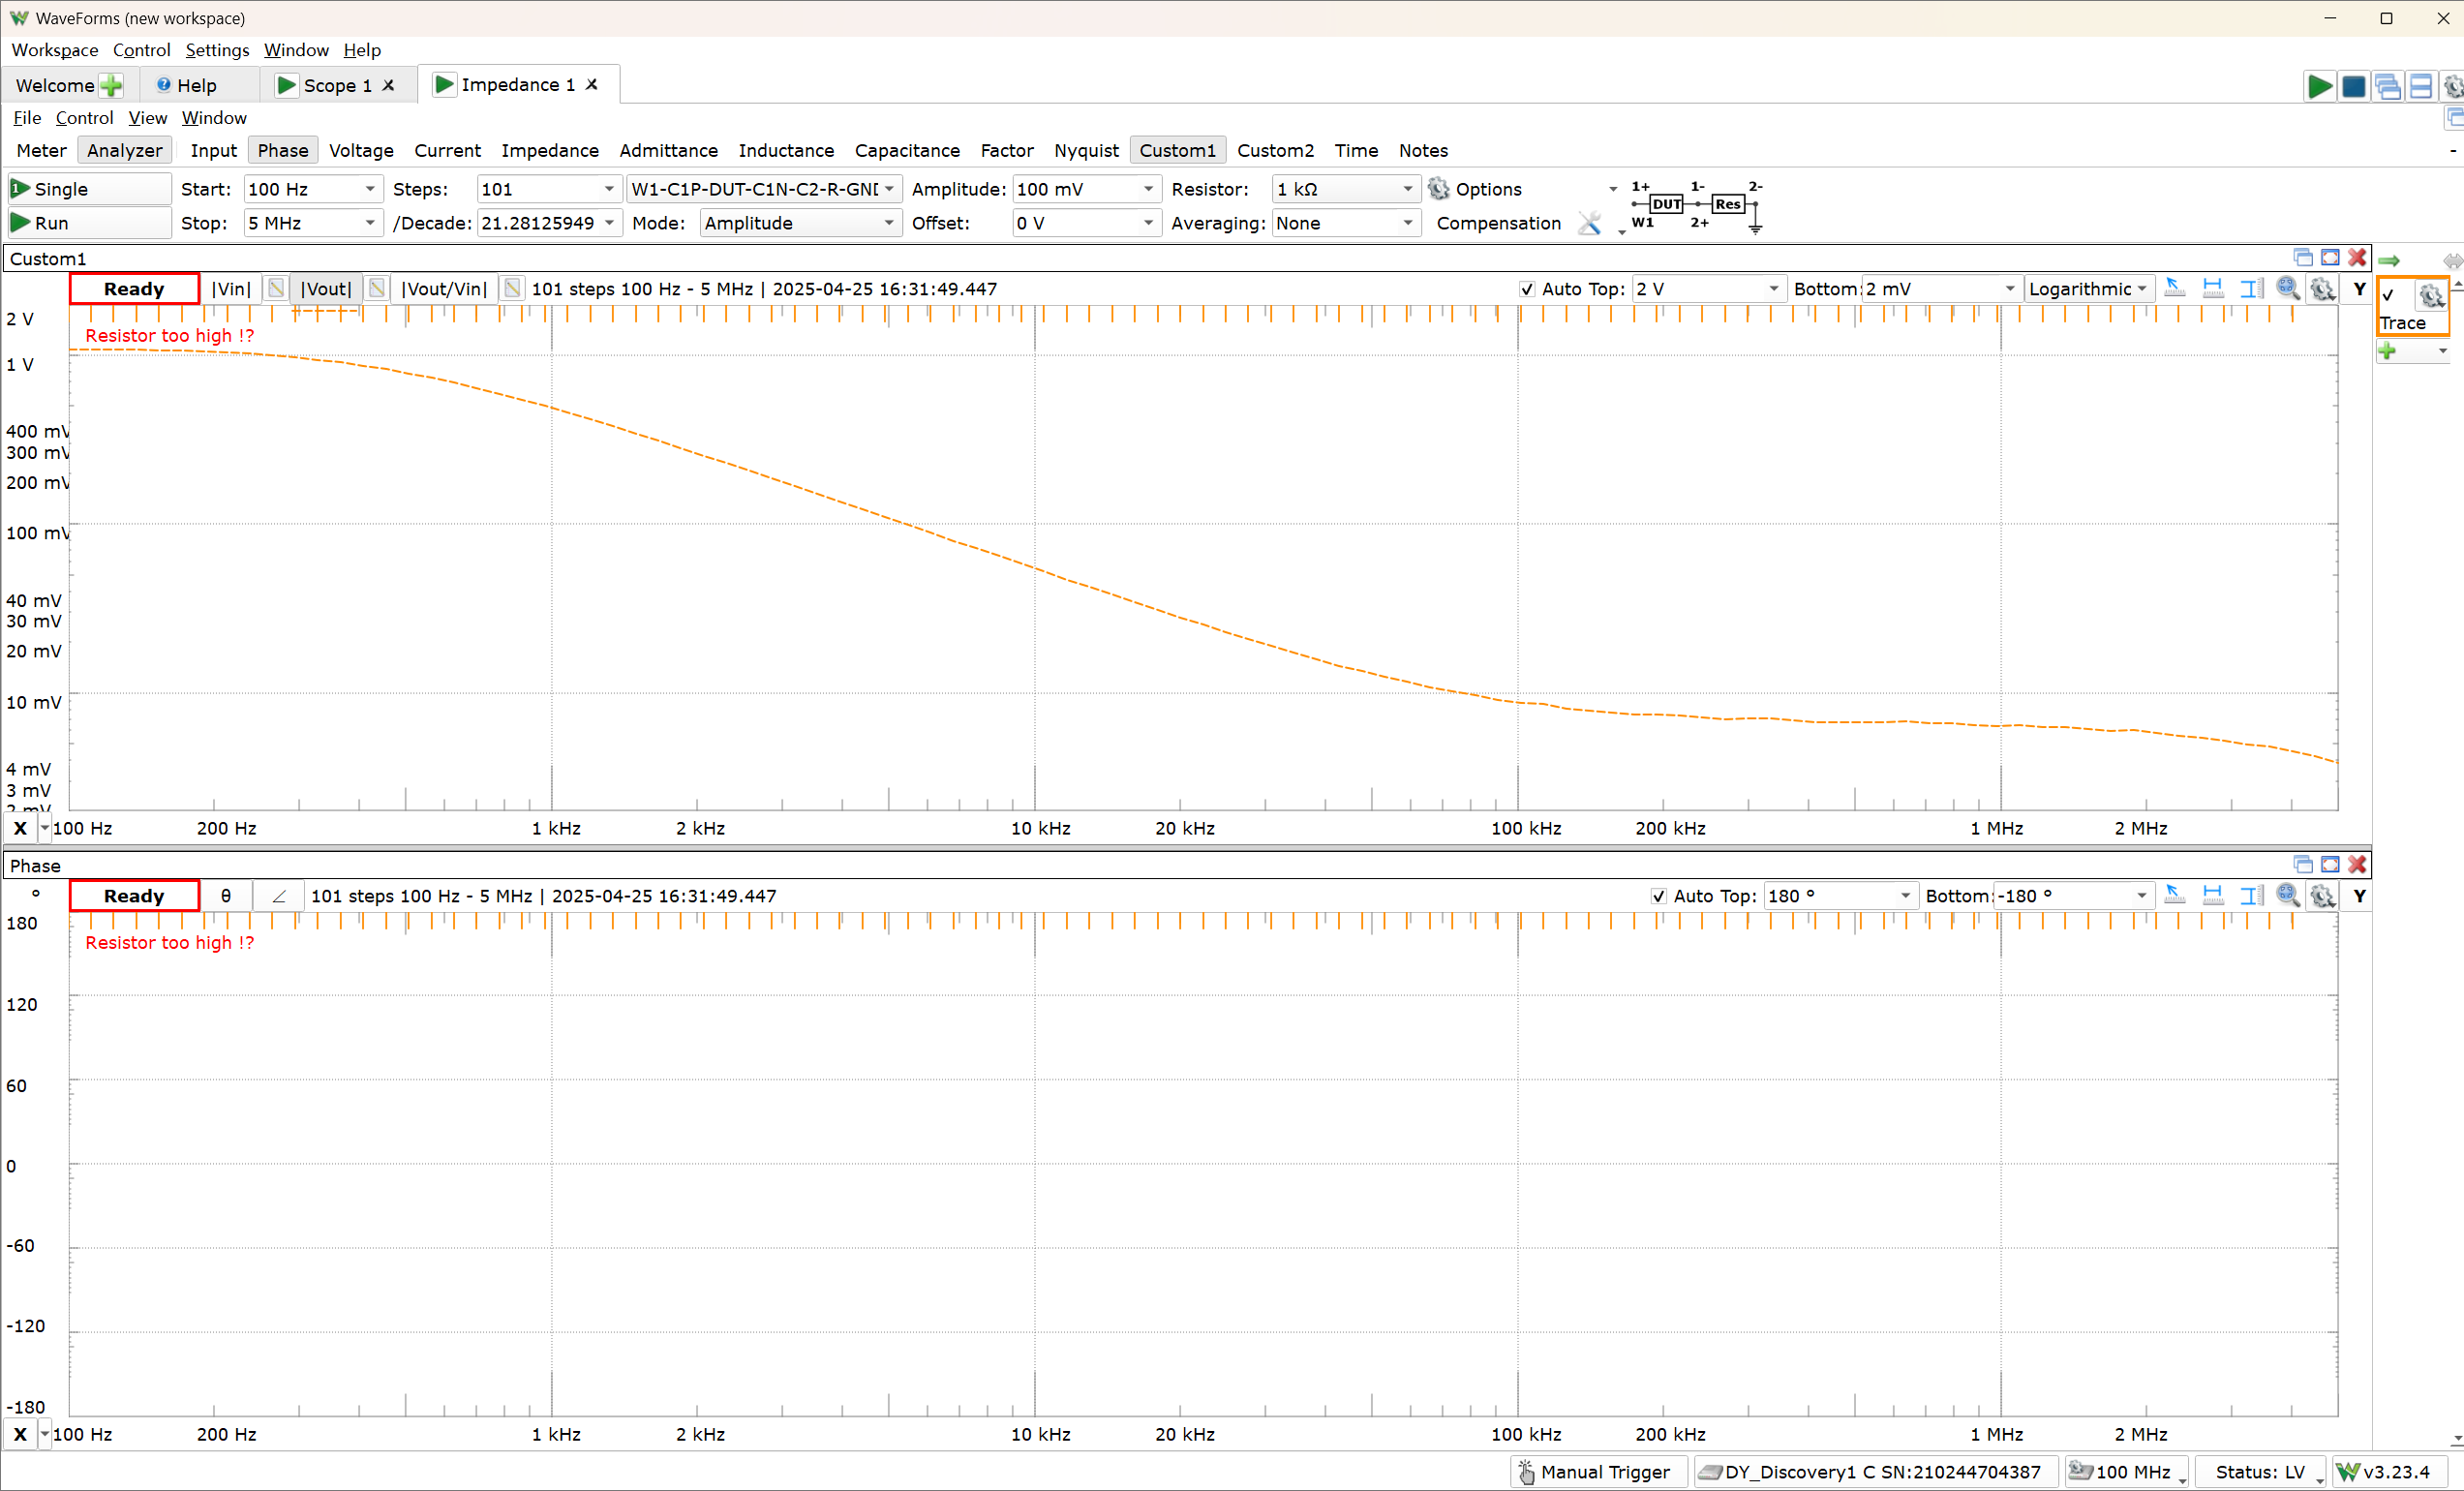
\includegraphics[width=\columnwidth]{LCE-04-场效应管/assets/cs amp/cs amp input impedance, R_S = 2M229 (input 100 mVamp, 100Hz ~ 5MHz).png}
    \caption{Common-source amp. frequency response: input 100 mVamp from 100 Hz to 5 MHz, $Z_L = 0,\ R_S = 2.229 \ \mathrm{M}\Omega$}
\end{figure}

输入部分的等效电路如下:
\begin{figure}[H]\centering
    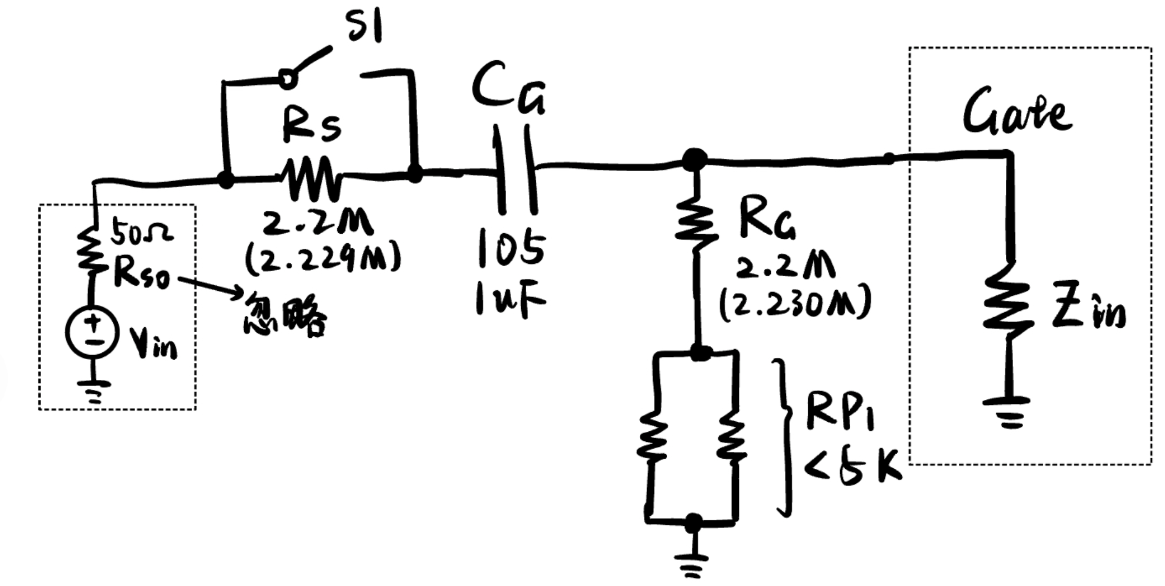
\includegraphics[width=0.6\columnwidth]{LCE-04-场效应管/assets/cs amp/input.png}
    \caption{放大器等效输入电路}
\end{figure}
当 $A_1$ 和 $A_2$ 已知时,忽略信号源的输出电阻 $R_{S0}$、电位器 $R_{P1}$ 以及电容 $C_{in} = 1 \ \mathrm{uF}$ 带来的影响 ($|Z_{C_{in}}| = 1.6 \ \mathrm{k}\Omega$ @ 100 Hz),容易推得:
\begin{gather}
Z = \frac{1}{\frac{\frac{A_1}{A_2} - 1}{R_S} - \frac{1}{R_G}}
\end{gather}
式中电阻实测值为 $R_S = 2.229 \ \mathrm{M}\Omega,\ R_G = 2.230 \ \mathrm{M}\Omega$。为了保证测量精度,我们并没有在输入端接入探头,也就没有相位数据,实际得到的是数据 $|A_2|$。因此,需要利用近似:
\begin{gather}
\label{eq: Z_in}
|Z|\approx  \frac{1}{\frac{\frac{|A_1|}{|A_2|} - 1}{R_S} - \frac{1}{R_G}}
\end{gather}
上式在 $A_1$ 和 $A_2$ 相位差不大时近似成立。



\subsubsection{增益曲线、输出阻抗曲线、输入阻抗曲线计算结果}

在 MATLAB 中利用公式 (\ref{eq: Z_out}) 和 (\ref{eq: Z_in}) 计算出 $Z_{out}$ 和 $|Z_{in}|$,并作出相关图像\footnote{
MATLAB 源码见附录 C 。
},结果如下:

\begin{figure}[H]\centering
    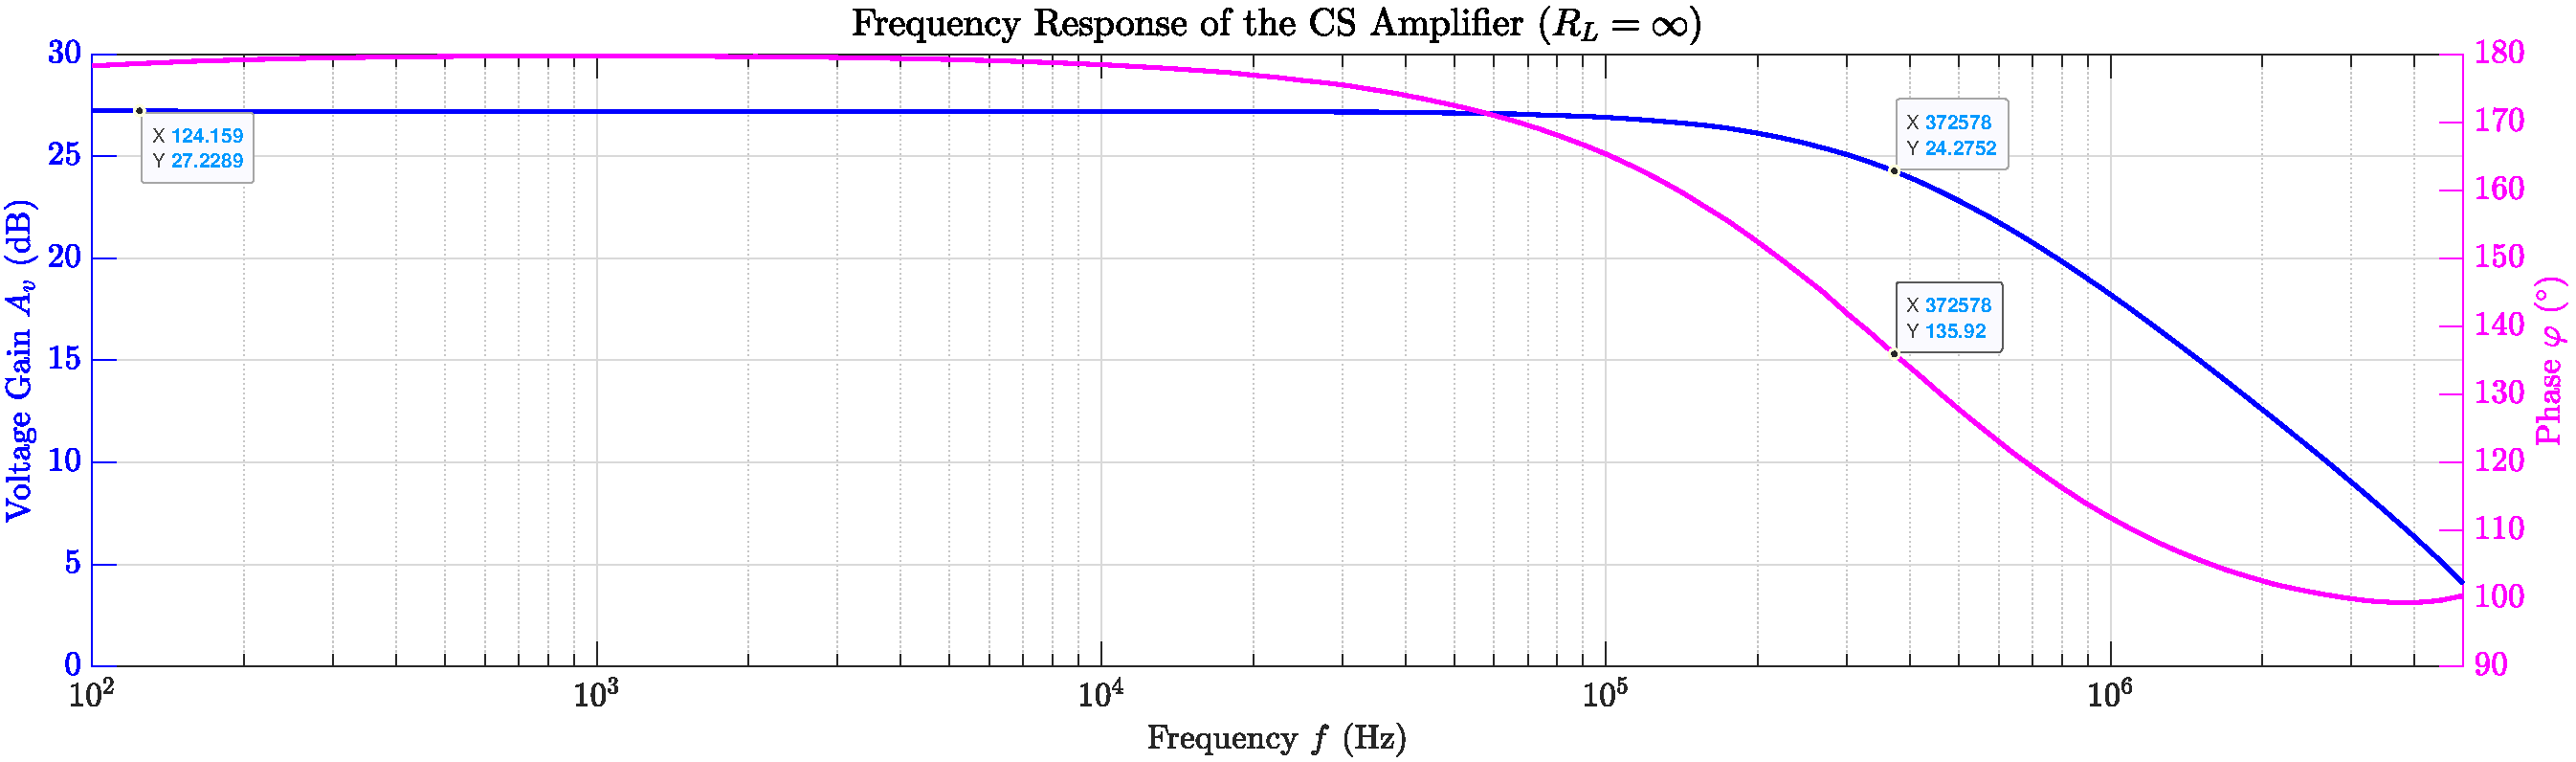
\includegraphics[width=\columnwidth]{LCE-04-场效应管/assets/cs amp/cs gain.pdf}
    \caption{Common-source amp. frequency response: input 100 mVamp from 100 Hz to 5 MHz, $Z_L = \infty,\ R_S = 0$}
\end{figure}

\begin{figure}[H]\centering
\begin{subfigure}[b]{0.5\columnwidth}\centering
    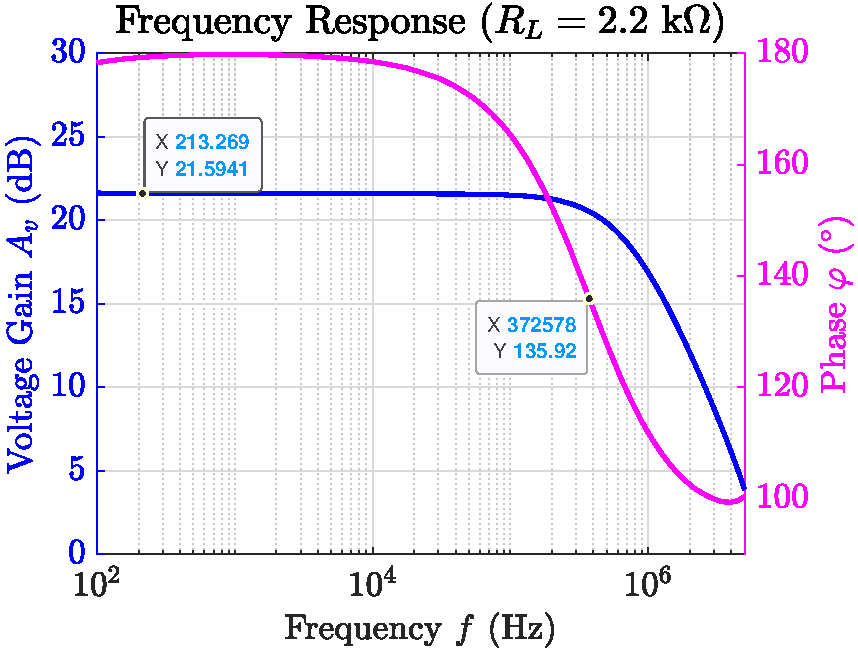
\includegraphics[width=220pt]{LCE-04-场效应管/assets/cs amp/cs gain, R_L = 2k2.pdf}
    \caption{Frequency response at $R_L = 2.2 \ \mathrm{k}\Omega$}
\end{subfigure}\hfill
\begin{subfigure}[b]{0.5\columnwidth}\centering
    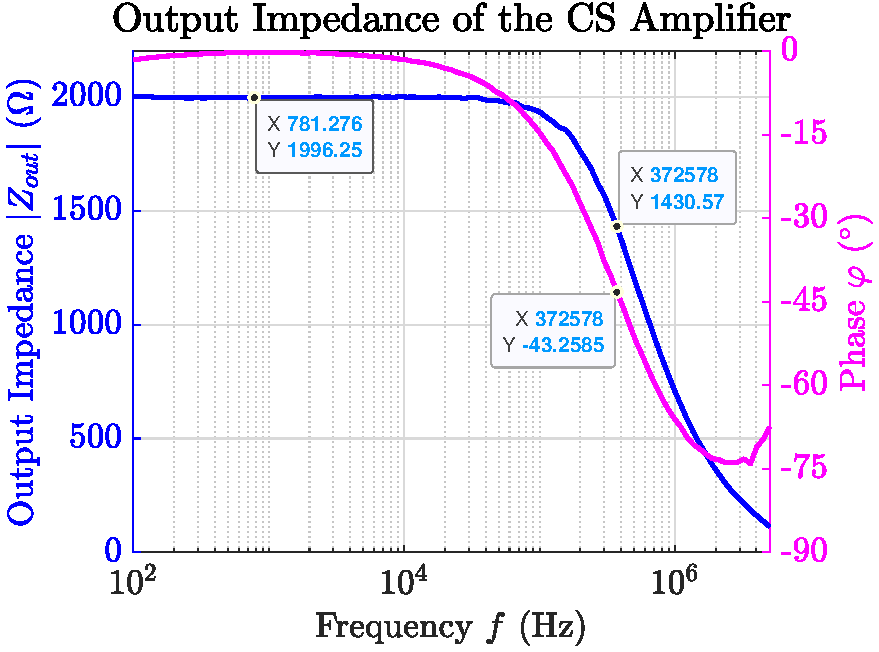
\includegraphics[width=220pt]{LCE-04-场效应管/assets/cs amp/cs Z_out.pdf}
    \caption{Output impedance curve $Z_{out} = Z_{out}(f)$}
\end{subfigure}
\caption{Common-source amp. frequency response:  at $R_L = 2.2 \ \mathrm{k}\Omega$ and the output impedance $Z_{out}$}
\end{figure}

\begin{figure}[H]\centering
\begin{subfigure}[b]{0.5\columnwidth}\centering
    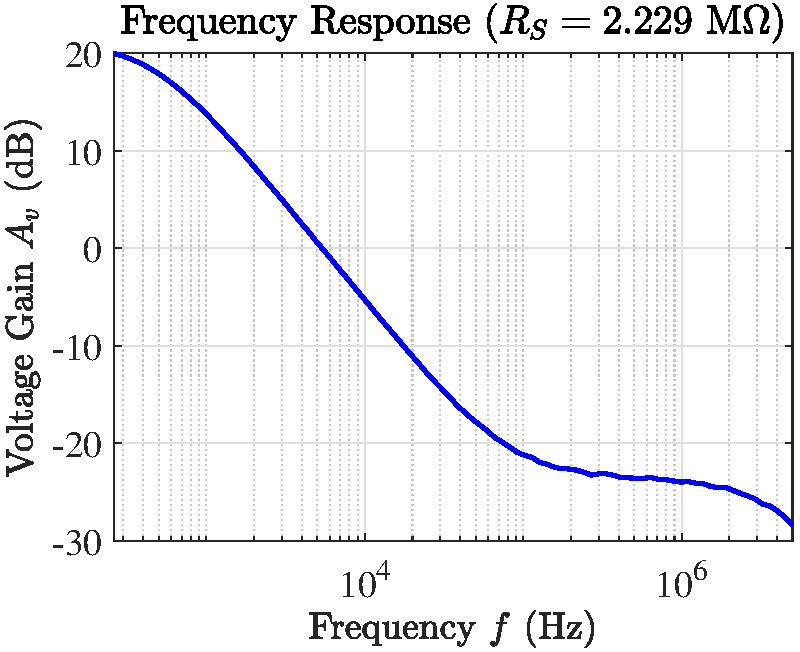
\includegraphics[width=210pt]{LCE-04-场效应管/assets/cs amp/cs gain, R_S = 2M229.pdf}\hspace*{8mm}
    \caption{Frequency response at $R_S = 2.229 \ \mathrm{M}\Omega$}
\end{subfigure}\hfill
\begin{subfigure}[b]{0.5\columnwidth}\centering
    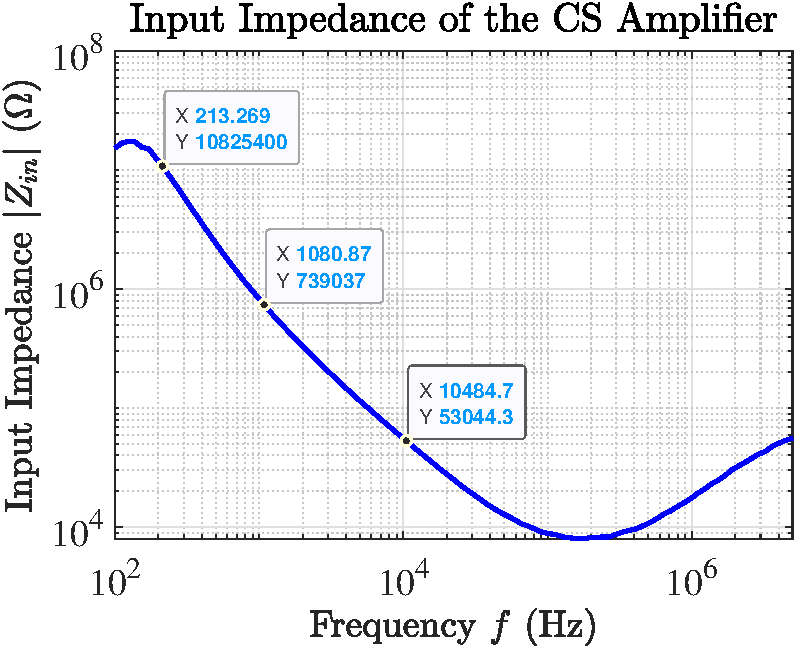
\includegraphics[width=210pt]{LCE-04-场效应管/assets/cs amp/cs Z_in.pdf}
    \hspace*{8mm}
    \caption{Input impedance curve $Z_{in} = Z_{in}(f)$}
\end{subfigure}
\caption{Common-source amp. frequency response:  at $R_S = 2.229 \ \mathrm{M}\Omega$ and the input impedance $Z_{in}$}
\end{figure}

\subsection{Common-Drain Amplifier (Source Follower)}

\subsubsection{设置静态工作点}

先断开全部跳线,然后闭合跳线 J1, J4, J7 构成 common-drain amplifier (source follower),在 CS Amp 中我们将晶体管电流设置在了约 3mA, 这里不妨重新调整为 14 mA, 对应 $R_{S2}$ 上的压降 6.02 V ,晶体管对应工作环境为:
\begin{gather}
I_D = 14 \ \mathrm{mA},\quad R_D = 0,\ R_{SS} = 430 \ \Omega
\end{gather}
我们实际将 $V_{R_{S2}}$ 调整到了 6.003 V, 对应 $I_D =  13.96 \ \mathrm{mA}$,此时 $V_{GS} = 2.513 \ \mathrm{V}$。

\subsubsection{测量频率响应 (原始增益曲线)}

AD1 的 W1 接 TP3, 通过电容 $C_G$ 将信号输入到 MOSFET 的 gate, AD1 的 CH1 和 CH2 分别接在 TP3 和 TP4 处,测量输入信号和输出信号,此时得到的曲线即为空载时的频率响应。设置信号源信号幅度为 2 Vamp (4 Vpp),得到输入输出波形如下:

\begin{figure}[H]\centering
    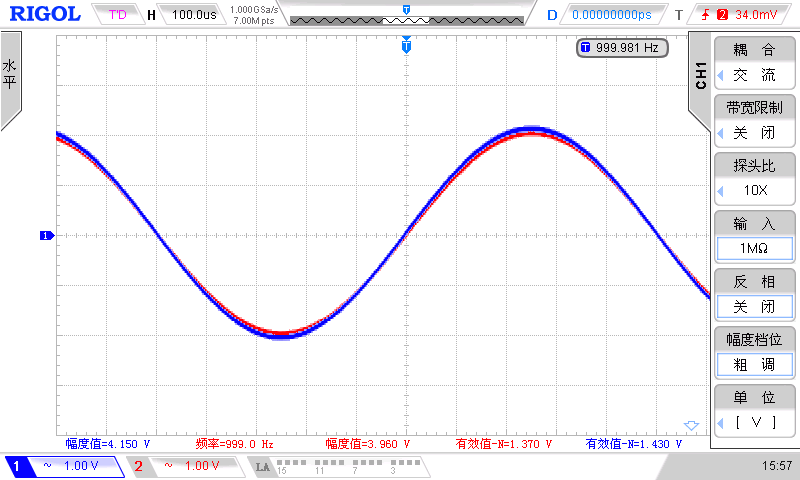
\includegraphics[width=\columnwidth]{LCE-04-场效应管/assets/cd amp/cd amp 输入输出波形 RIGOL.png}
    \caption{(RIGOL) cd amp. I/O waveform: input signal (CH1-blue, 2 Vamp @ 1 kHz), output signal (CH2-red), overlap display}
\end{figure}
\begin{figure}[H]\centering
    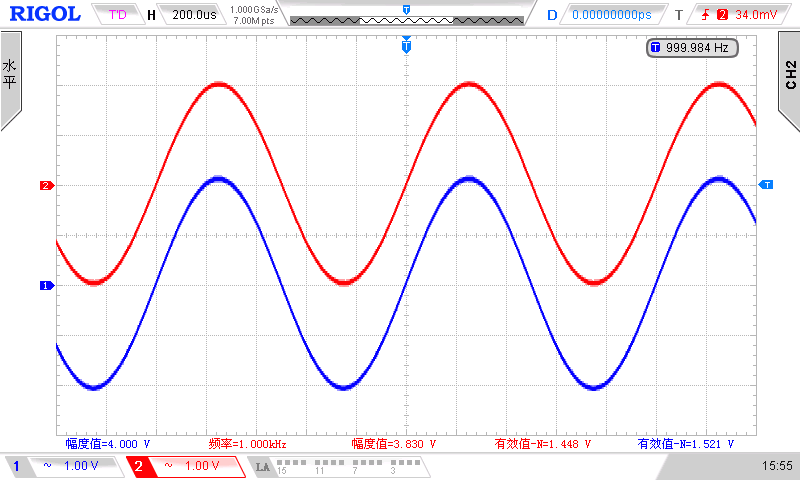
\includegraphics[width=\columnwidth]{LCE-04-场效应管/assets/cd amp/cd amp 输入输出波形 RIGOL (2).png}
    \caption{(RIGOL) cd amp. I/O waveform: input signal (CH1-blue, 2 Vamp @ 1 kHz), output signal (CH2-red), misaligned display}
\end{figure}
\begin{figure}[H]\centering
    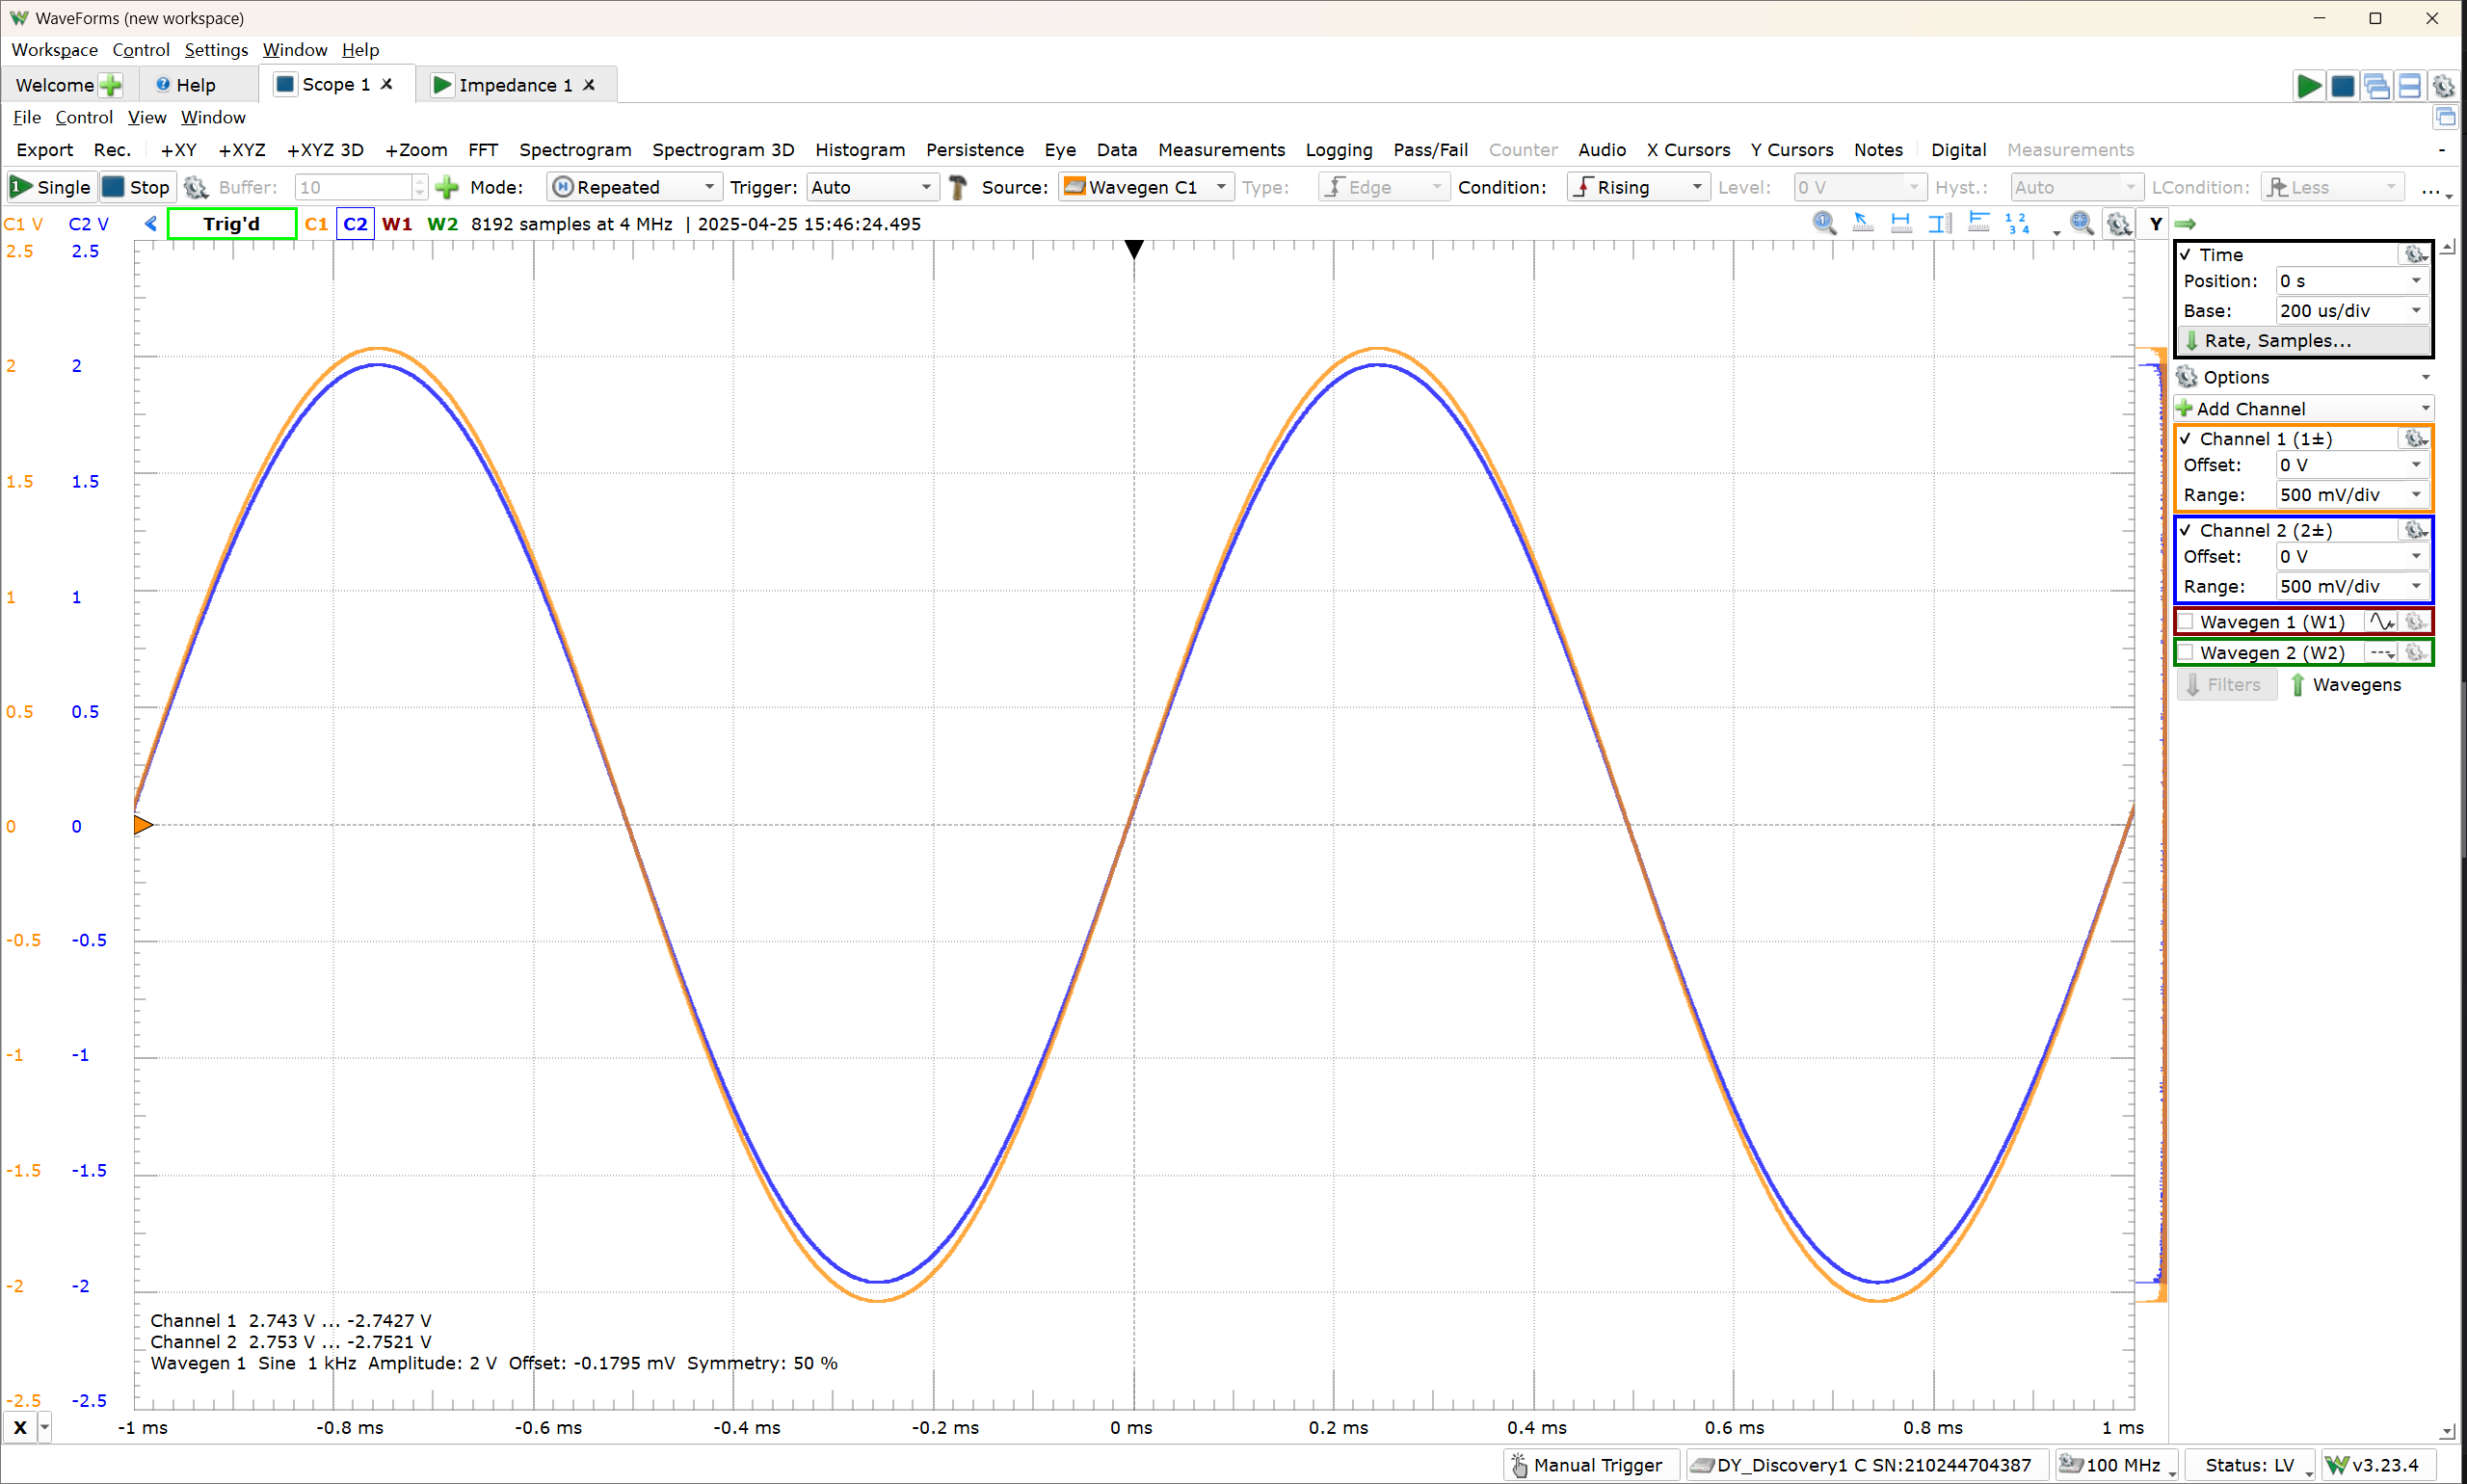
\includegraphics[width=\columnwidth]{LCE-04-场效应管/assets/cd amp/cd amp 输入输出波形.png}
    \caption{(AD1) cd amp. I/O waveform: input signal (CH1-orange, 2 Vamp @ 1 kHz), output signal (CH2-blue), overlap display}
\end{figure}
\begin{figure}[H]\centering
    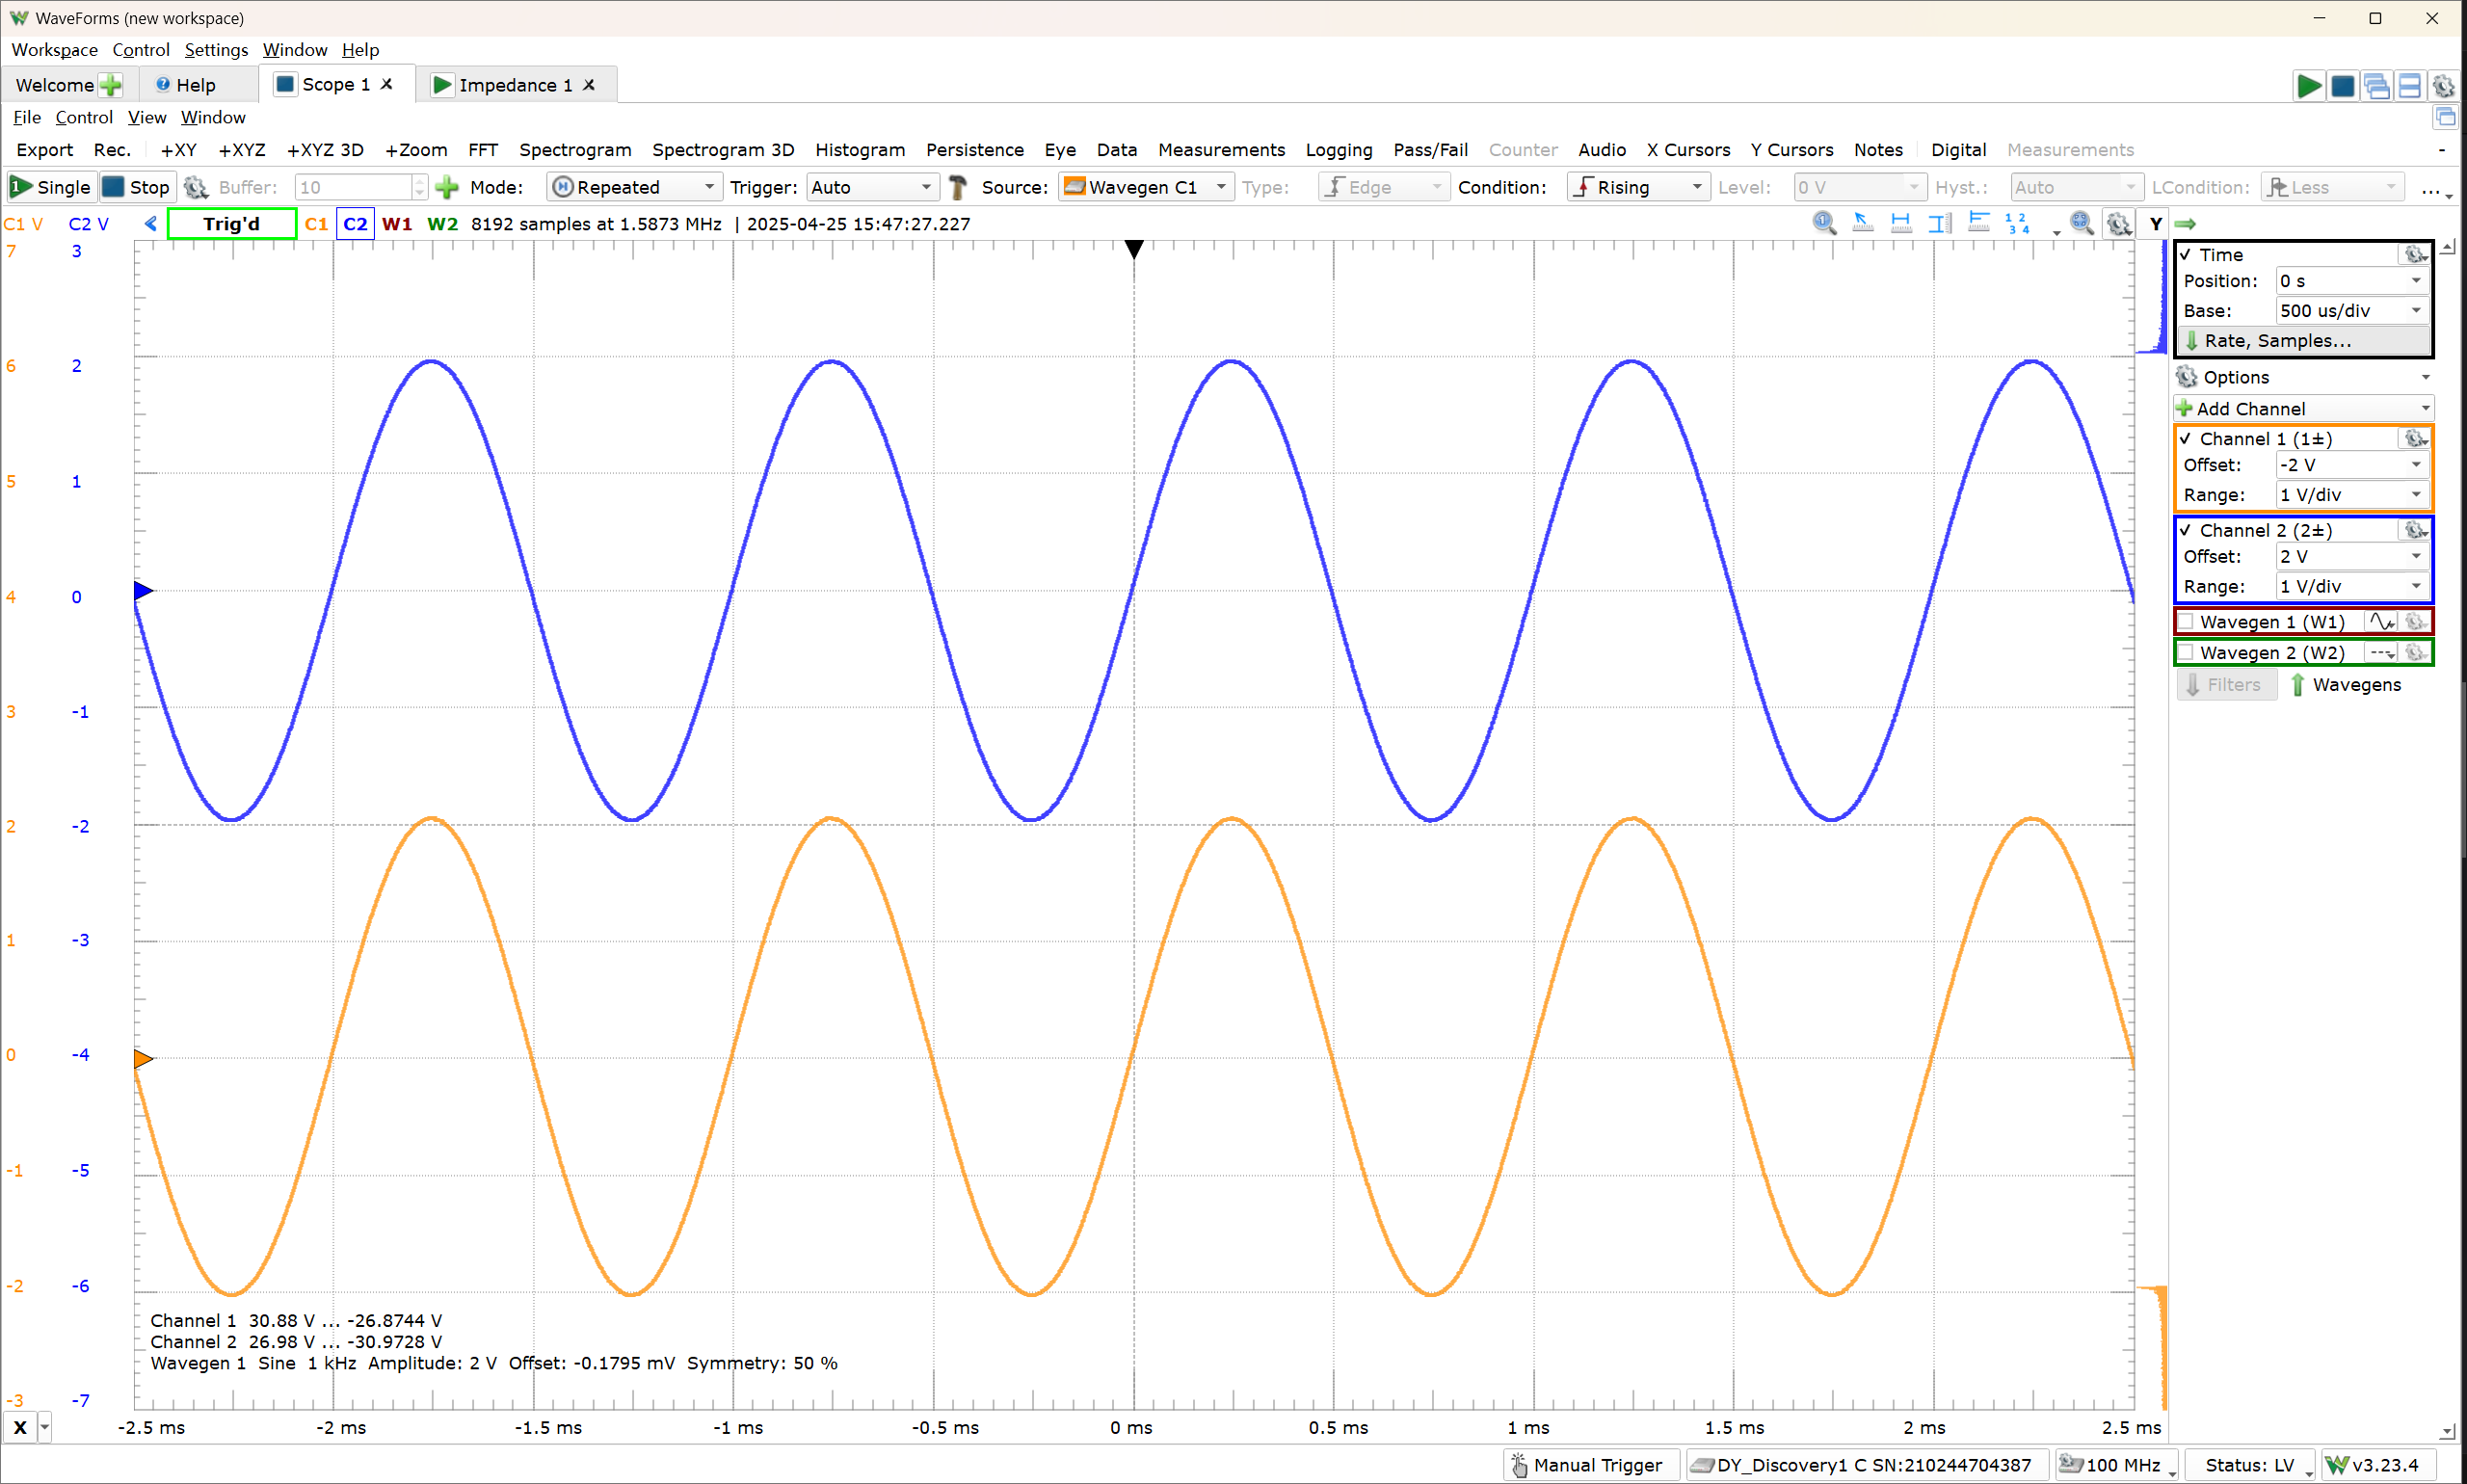
\includegraphics[width=\columnwidth]{LCE-04-场效应管/assets/cd amp/cd amp 输入输出波形 (2).png}
    \caption{(AD1) cd amp. I/O waveform: input signal (CH1-orange, 2 Vamp @ 1 kHz), output signal (CH2-blue), misaligned display}
\end{figure}

保持各设置不变,进行扫频分析,得到增益曲线如下:

\begin{figure}[H]\centering
    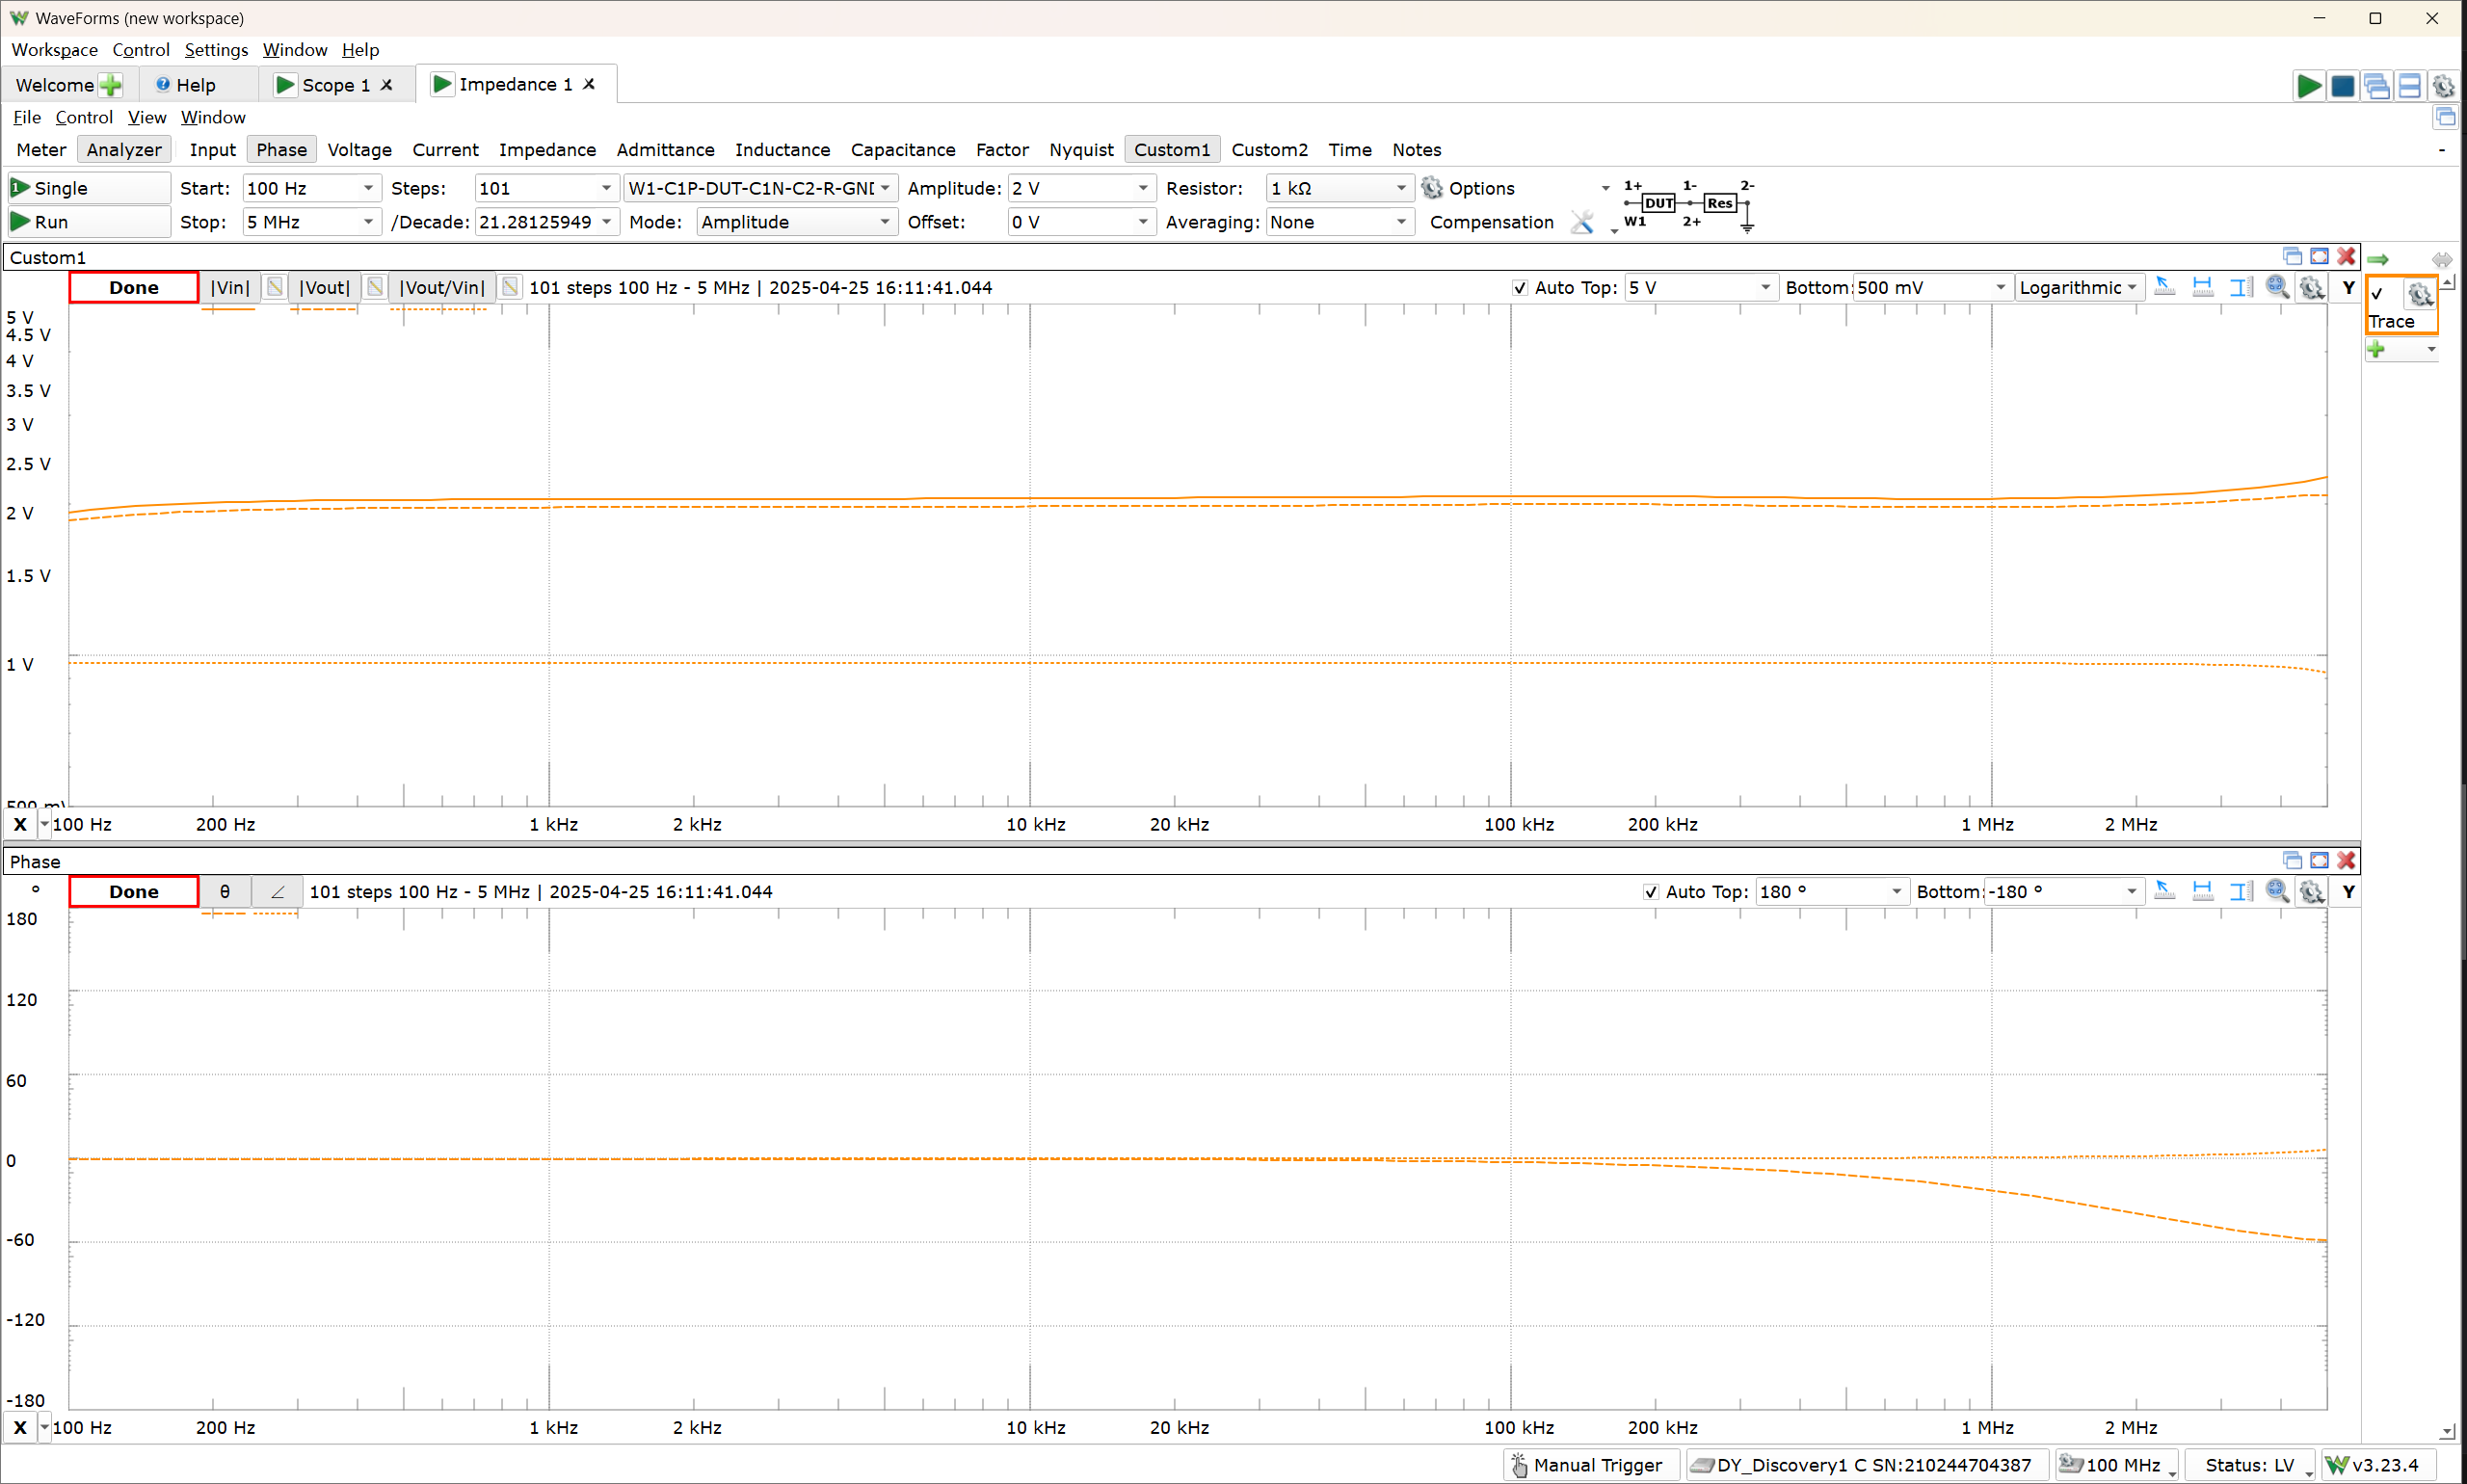
\includegraphics[width=\columnwidth]{LCE-04-场效应管/assets/cd amp/cd amp frequency response (input 2 Vamp, 100Hz ~ 5MHz).png}
    \caption{Common-drain amplifier frequency response: input 2 Vamp from 100 Hz to 5 MHz, $Z_L = \infty,\ R_S = 0$}
\end{figure}

从上图可以很容易看出 common-drain 的频率特性优于 common-source (从高频截止频率的角度),在我们设置的电路参数下,前者的高频截止频率 $f_c > 1 \ \mathrm{M}Hz$。

\newpage
\subsubsection{测量输出有负载时的增益}

闭合跳线 J11, 接入负载 $220 \ \mathrm{uF} + 100 \Omega$。保持输入信号幅度不变,仍在 TP4 进行测量,结果如下:
\begin{figure}[H]\centering
    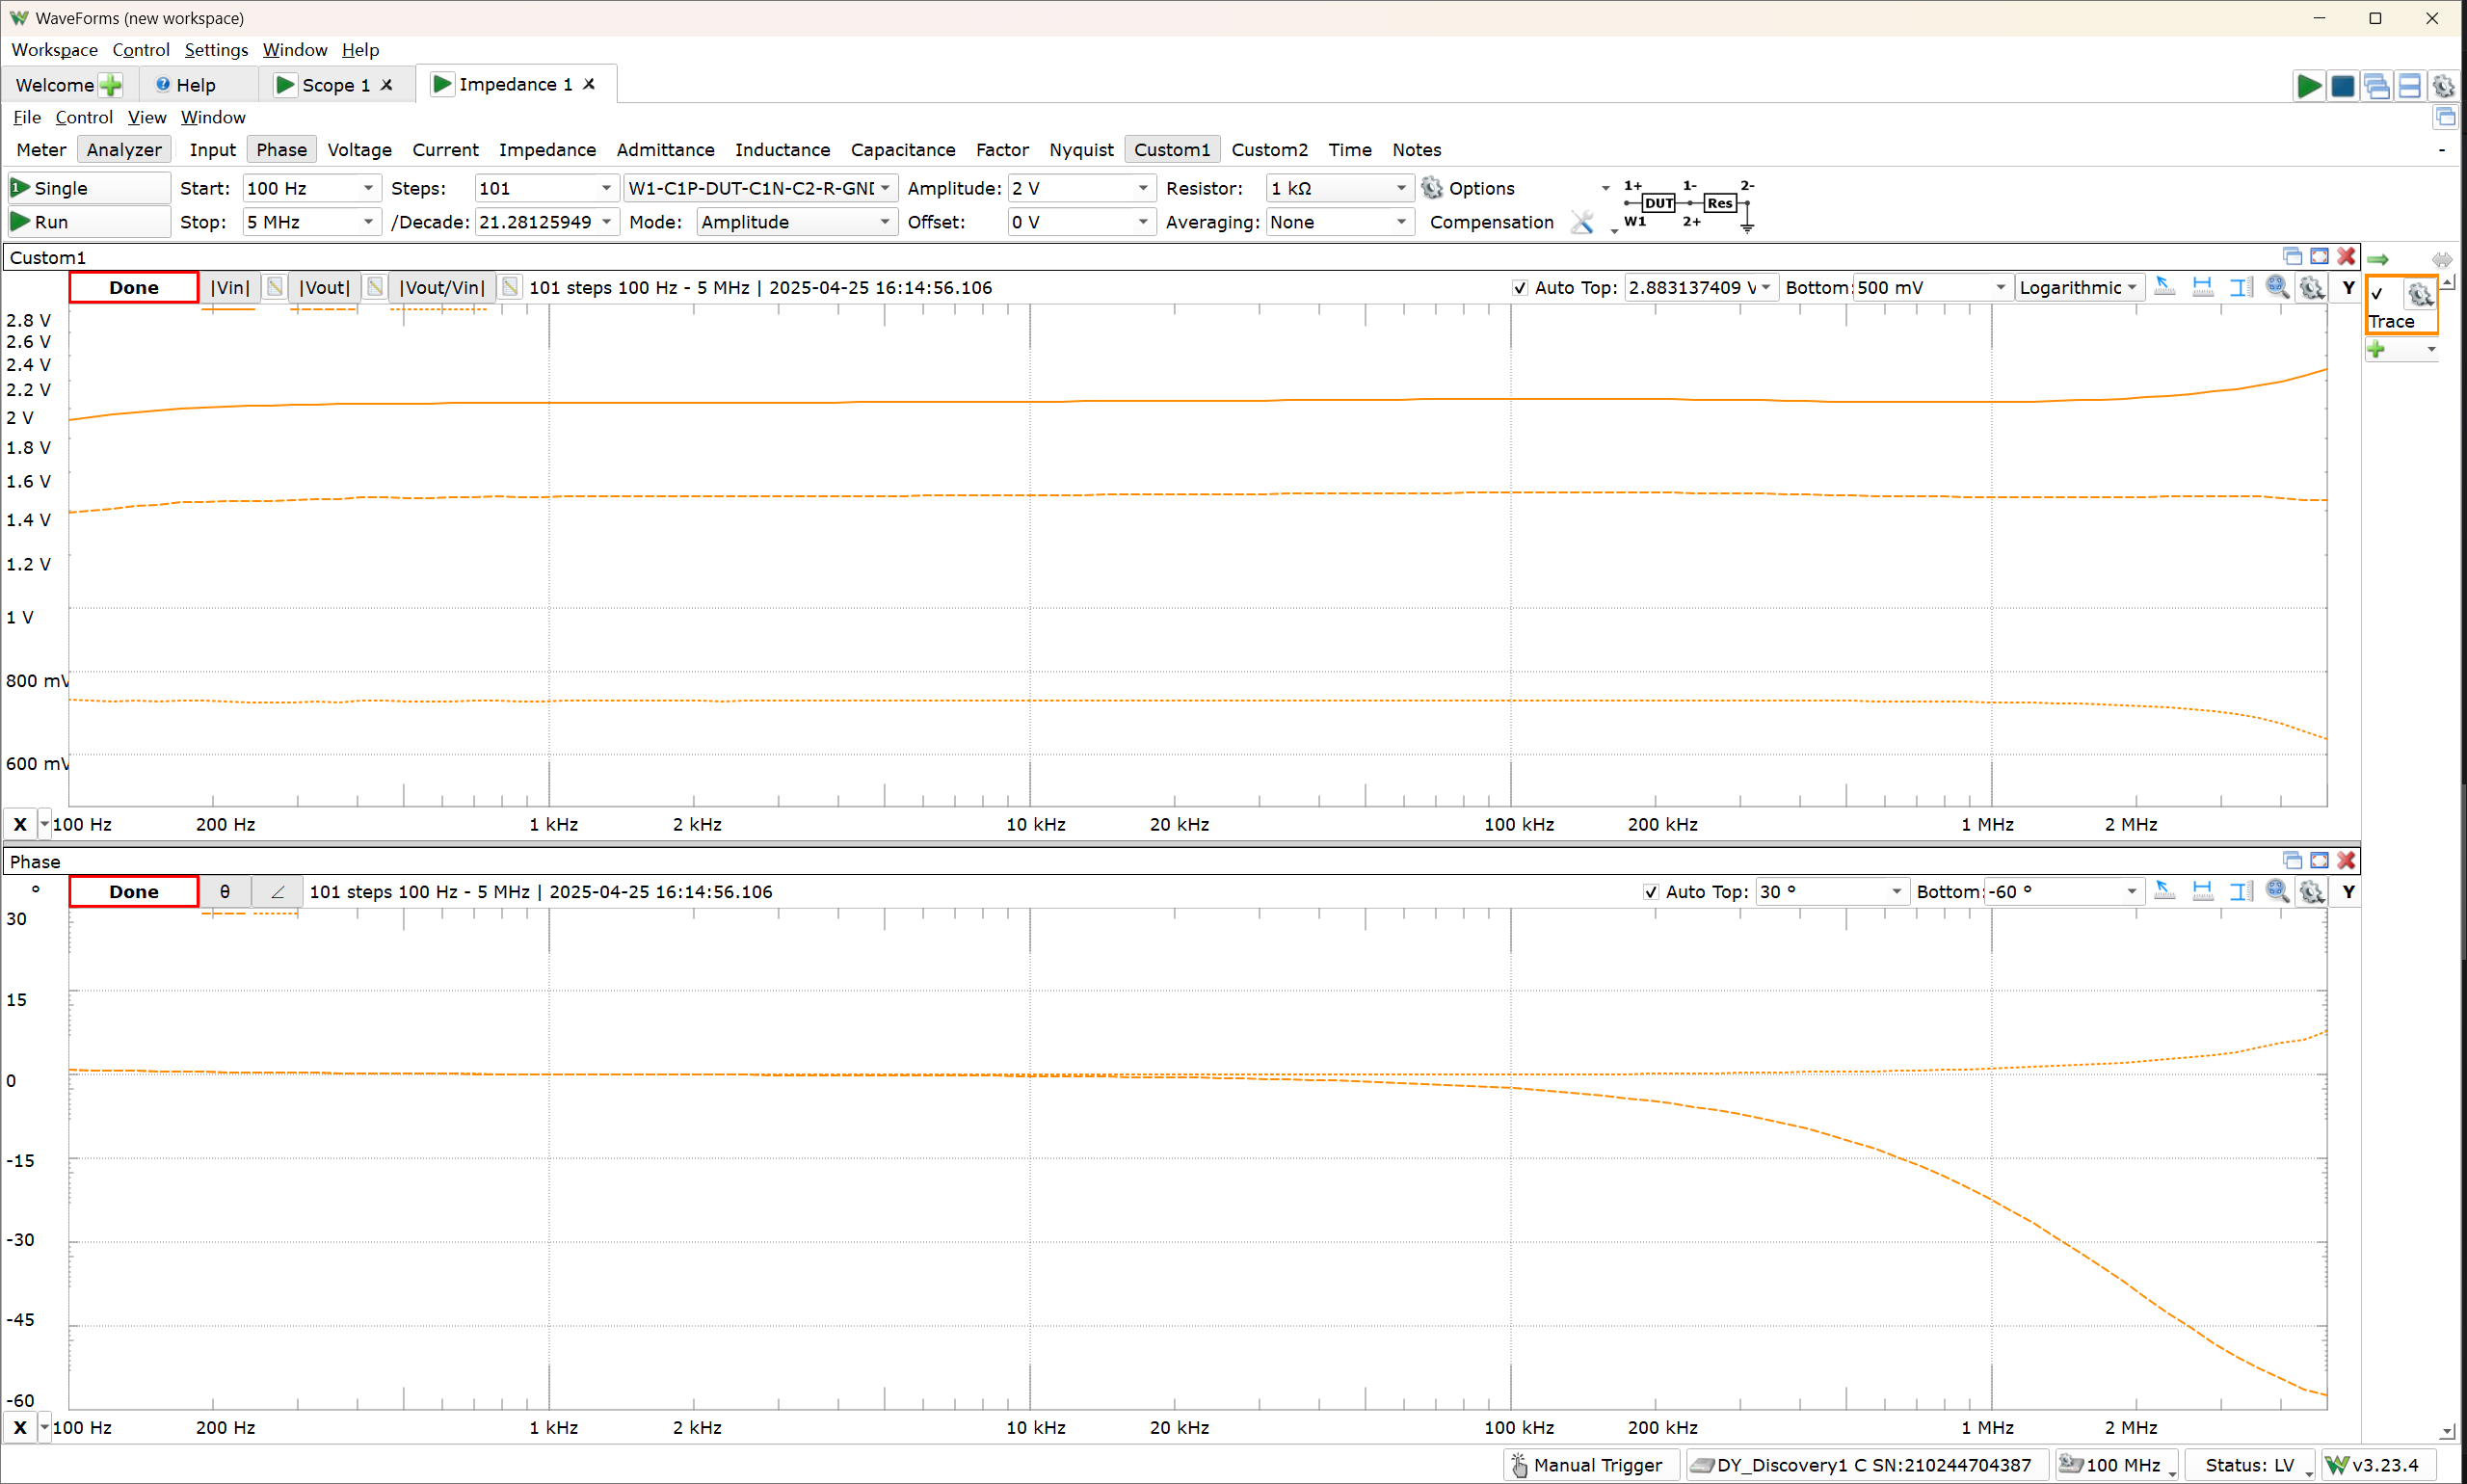
\includegraphics[width=0.97\columnwidth]{LCE-04-场效应管/assets/cd amp/cd amp output impedance, R_L = 100 Ohm (input 2 Vamp, 100Hz ~ 5MHz).png}
    \caption{Common-drain amp. frequency response: input 2 Vamp from 100 Hz to 5 MHz, $Z_L = 22 \ \mathrm{uF} + 2.2 \ \mathrm{k}\Omega,\ R_S = 0$}
\end{figure}

\subsubsection{测量输入有分压时的增益}

断开负载跳线 J11, 断开输入分压电阻的跳线 J1, 得到频率响应曲线如下:
\begin{figure}[H]\centering
    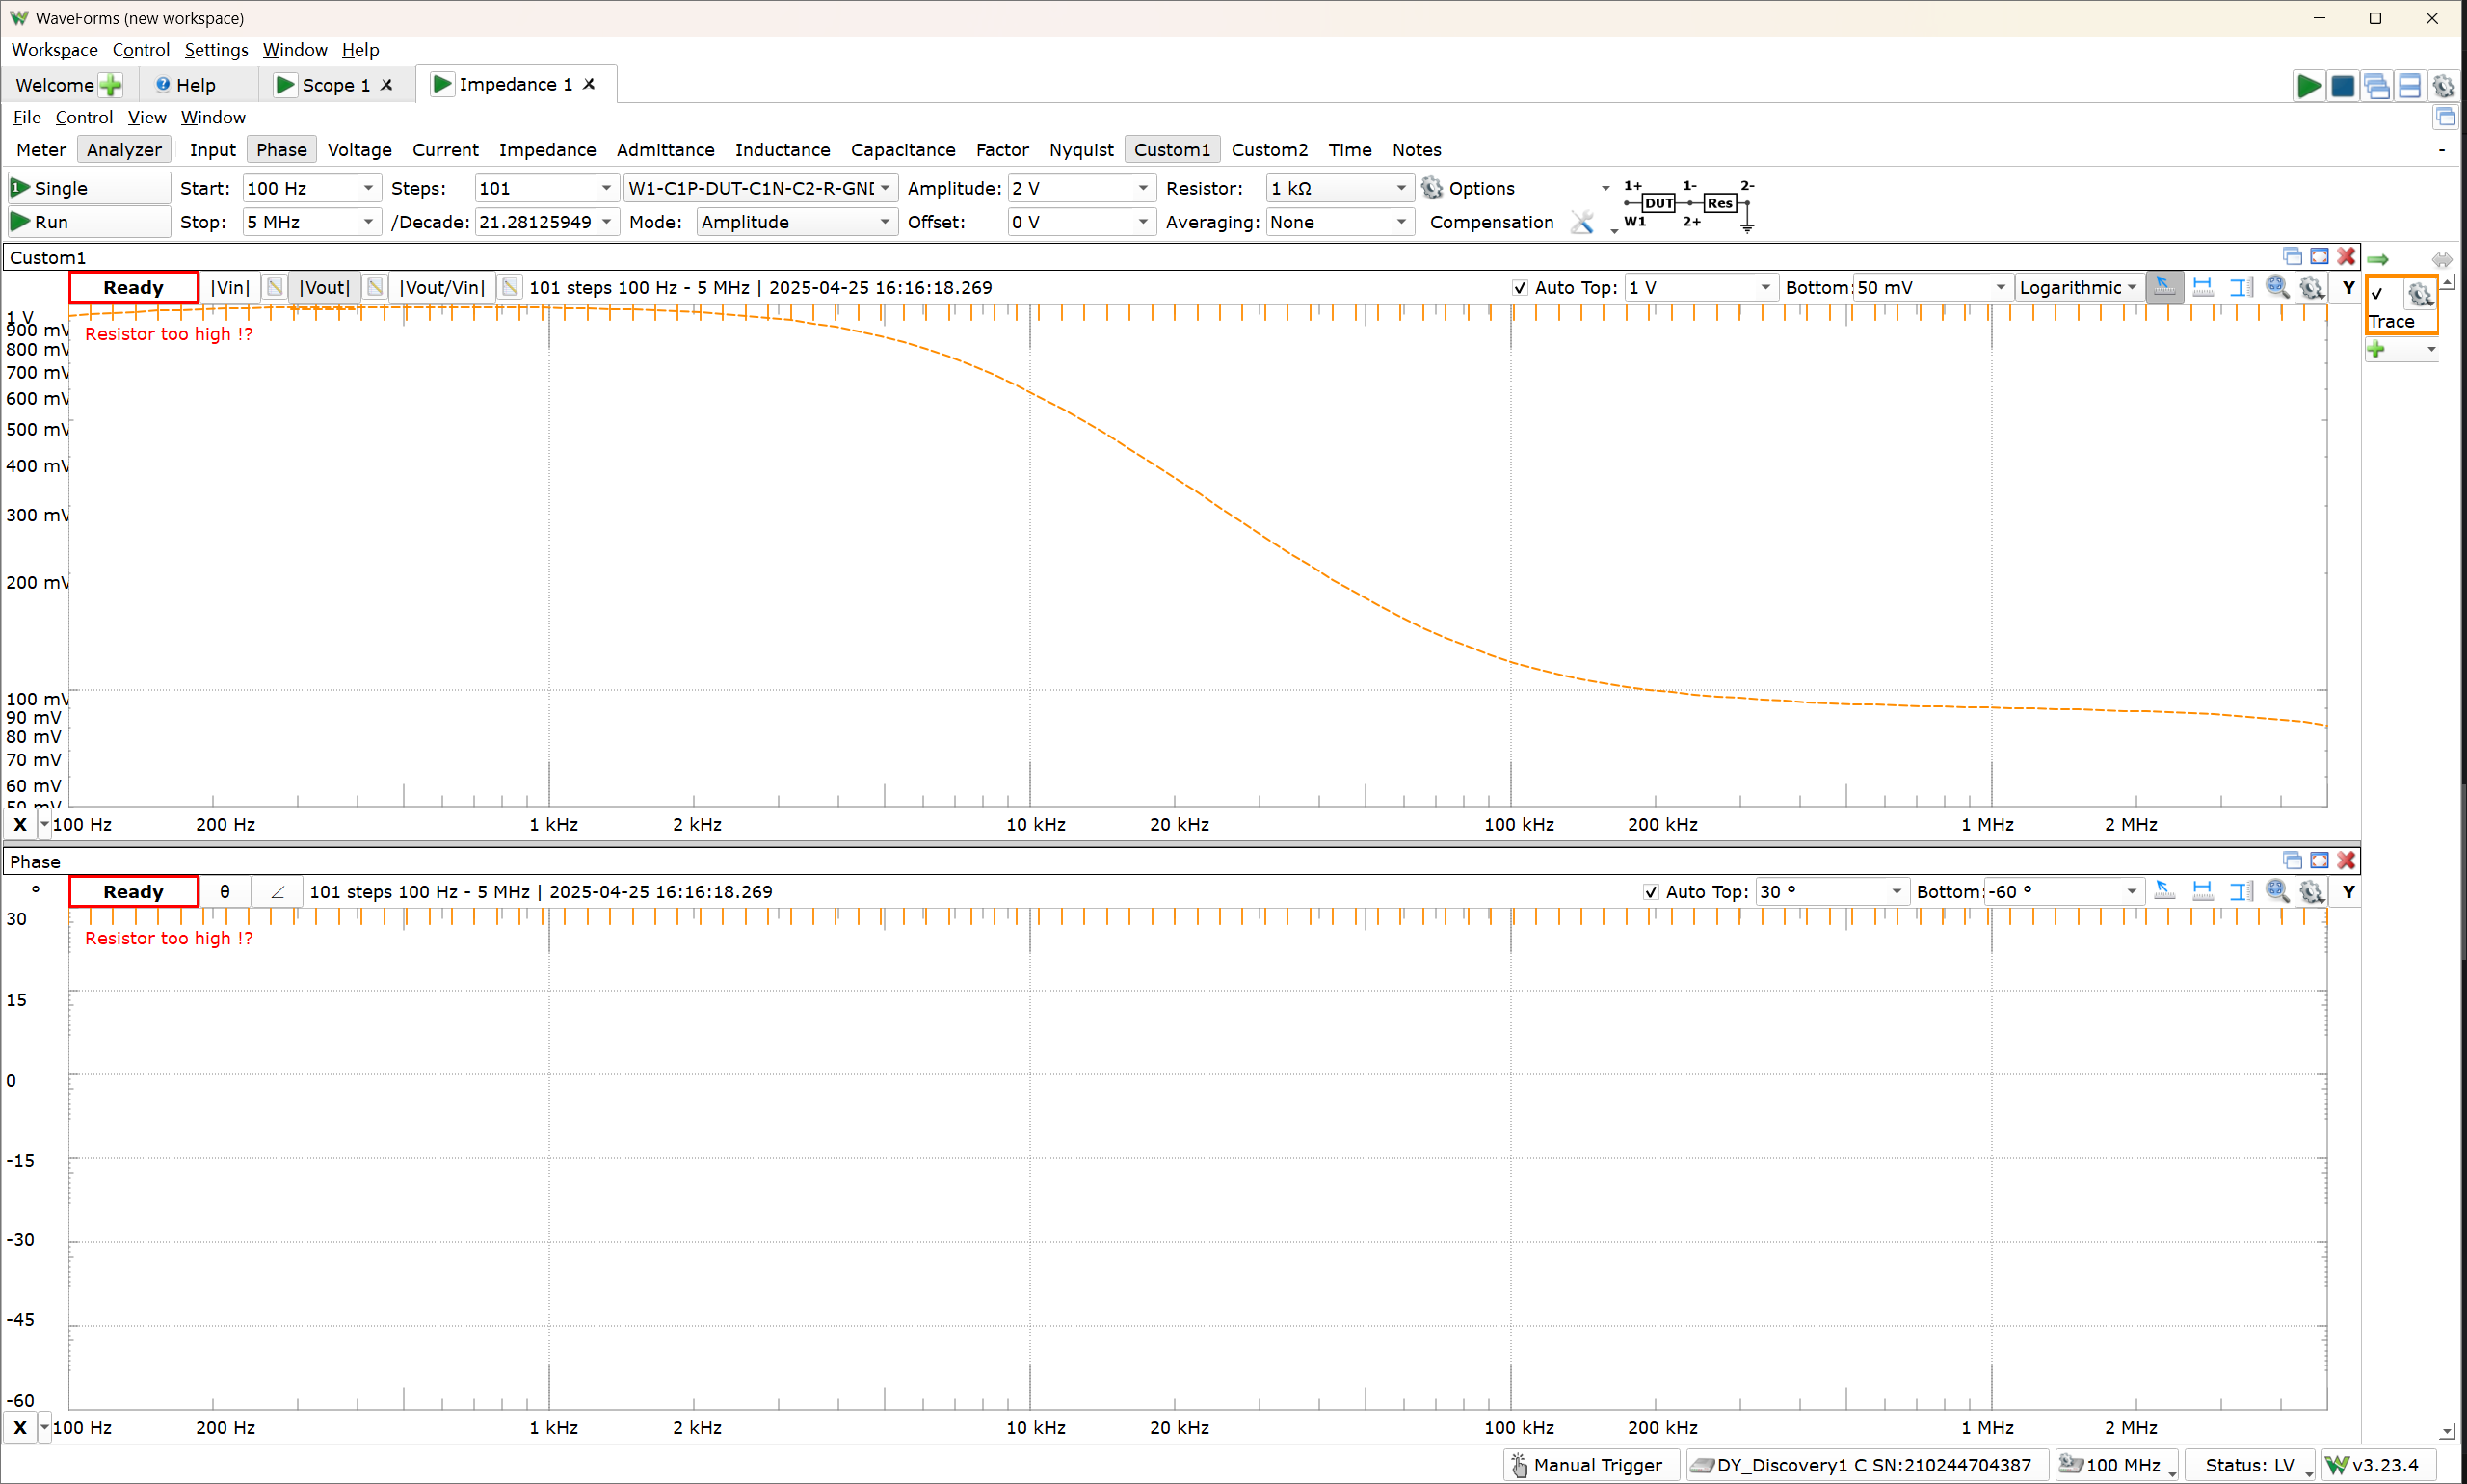
\includegraphics[width=0.97\columnwidth]{LCE-04-场效应管/assets/cd amp/cd amp input impedance, R_S = 2M229 (input 2 Vamp, 100Hz ~ 5MHz).png}
    \caption{Common-drain amp. frequency response: input 2 Vamp from 100 Hz to 5 MHz, $Z_L = 0,\ R_S = 2.229 \ \mathrm{M}\Omega$}
\end{figure}

\subsubsection{增益曲线、输出阻抗曲线、输入阻抗曲线计算结果}

类似地,利用公式 (\ref{eq: Z_out}) 和 (\ref{eq: Z_in}) 计算出 $Z_{out}$ 和 $|Z_{in}|$,作出相关图像如下:


\begin{figure}[H]\centering
    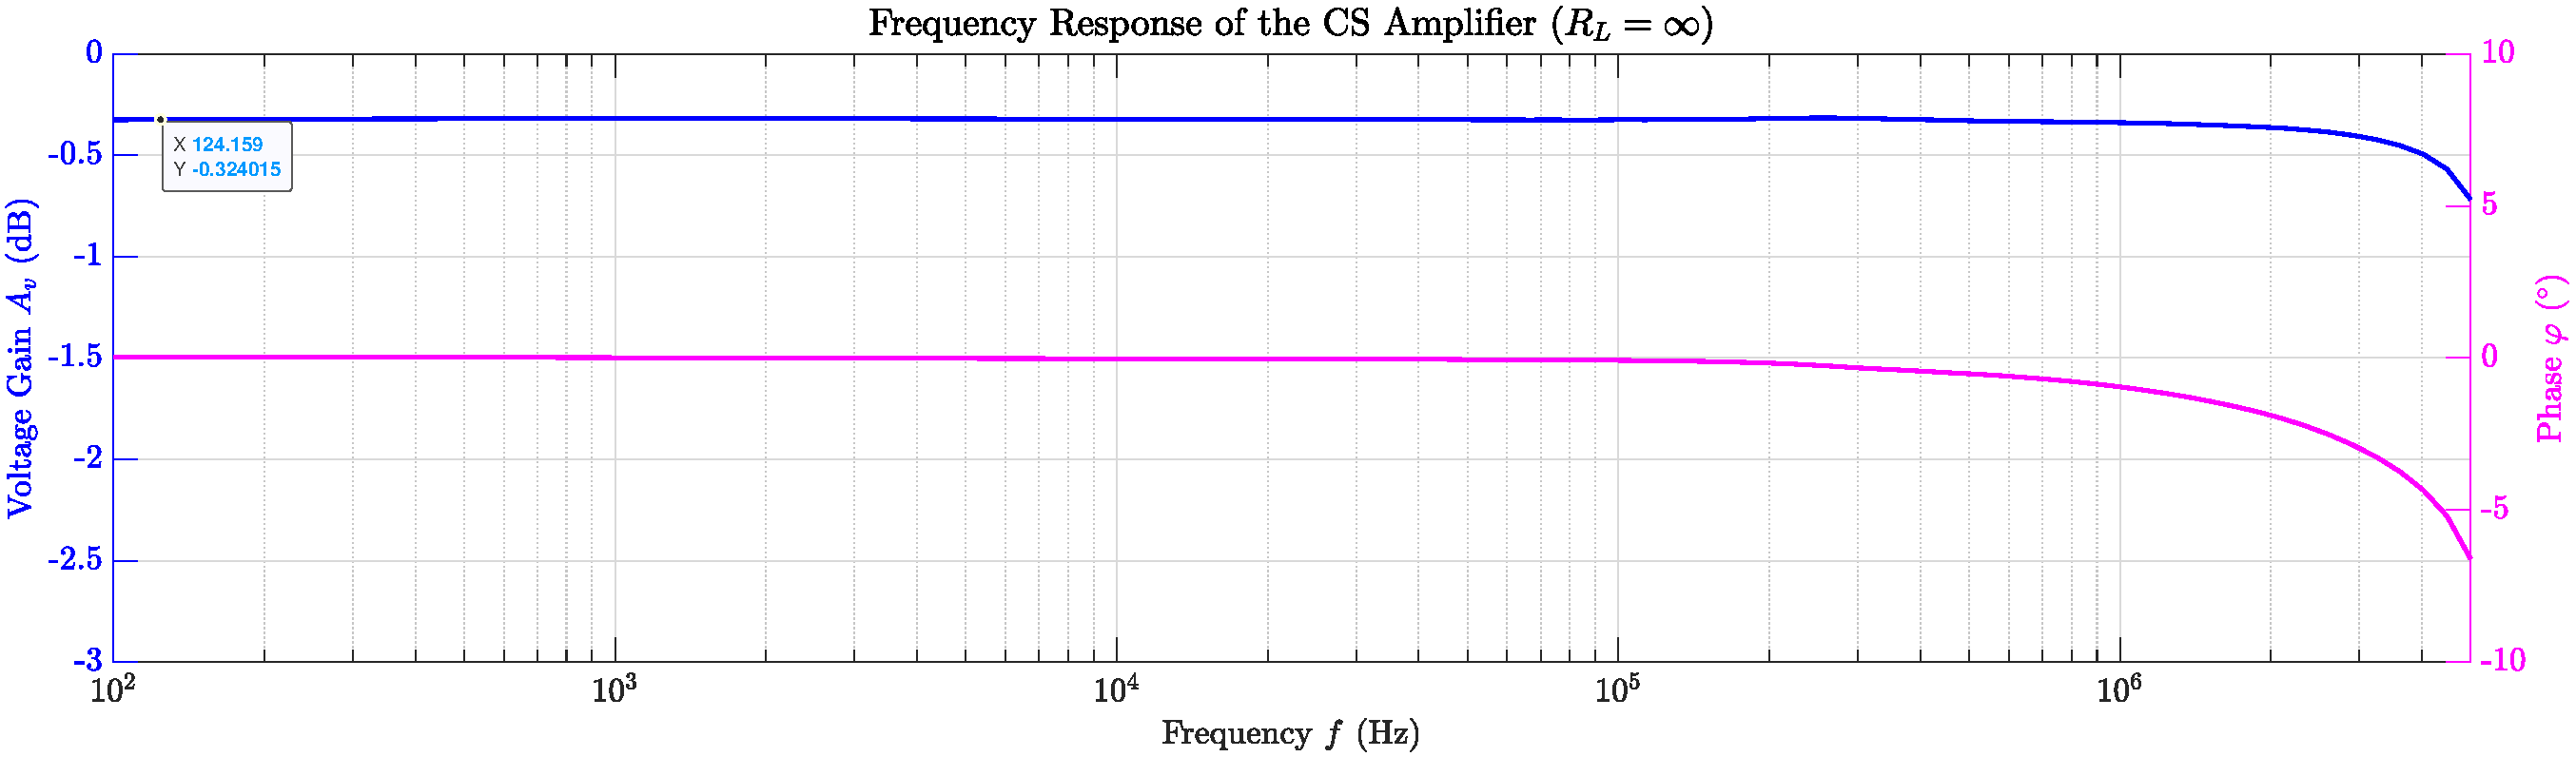
\includegraphics[width=\columnwidth]{LCE-04-场效应管/assets/cd amp/cd gain.pdf}
    \caption{Common-drain amp. frequency response: input 2 Vamp from 100 Hz to 5 MHz, $Z_L = \infty,\ R_S = 0$}
\end{figure}
\vspace*{-3mm}
\begin{figure}[H]\centering
\begin{subfigure}[b]{0.5\columnwidth}\centering
    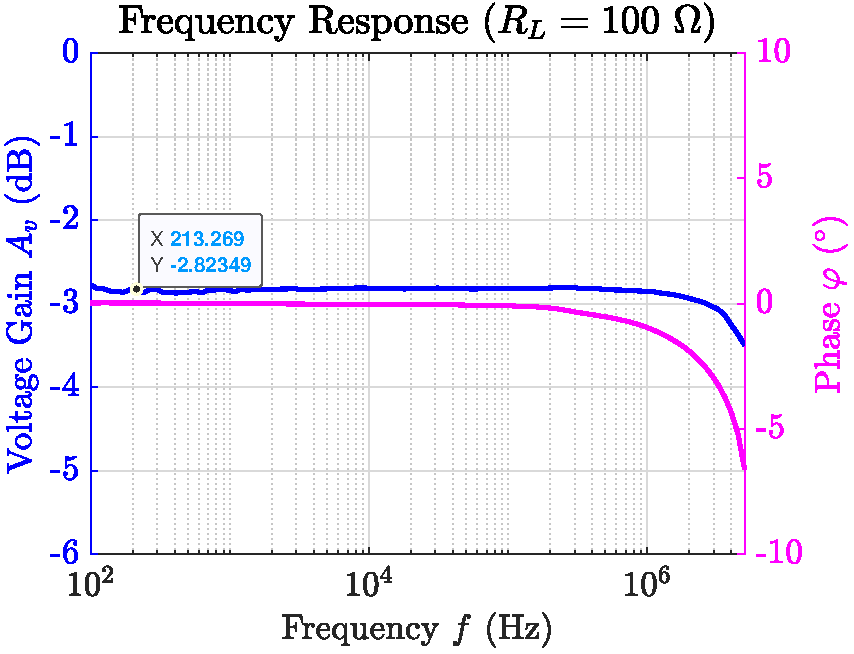
\includegraphics[width=220pt]{LCE-04-场效应管/assets/cd amp/cd gain, R_L = 100.pdf}
    \caption{Frequency response at $R_L = 100\ \Omega$}
\end{subfigure}\hfill
\begin{subfigure}[b]{0.5\columnwidth}\centering
    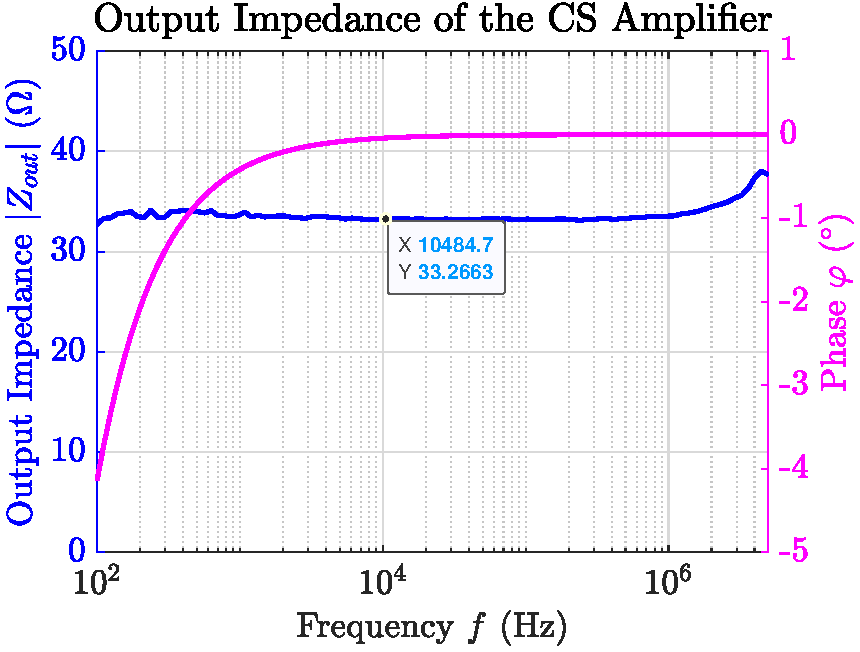
\includegraphics[width=220pt]{LCE-04-场效应管/assets/cd amp/cd Z_out.pdf}
    \caption{Output impedance curve $Z_{out} = Z_{out}(f)$}
\end{subfigure}
\caption{Common-drain amp. frequency response:  at $R_L = 100 \ \Omega$ and the output impedance $Z_{out}$}
\end{figure}
\vspace*{-3mm}
\begin{figure}[H]\centering
\begin{subfigure}[b]{0.5\columnwidth}\centering
    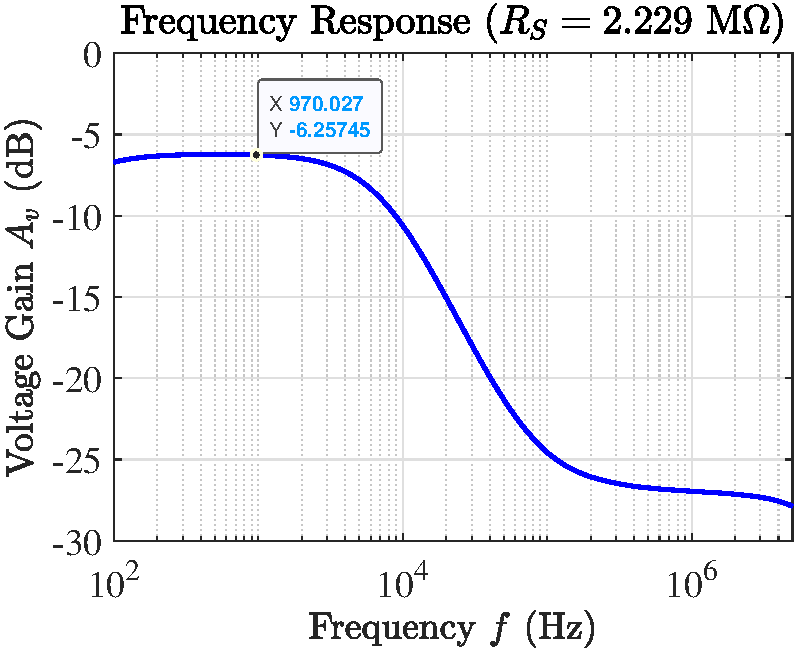
\includegraphics[width=210pt]{LCE-04-场效应管/assets/cd amp/cd gain, R_S = 2M229.pdf}\hspace*{8mm}
    \caption{Frequency response at $R_S = 2.229 \ \mathrm{M}\Omega$}
\end{subfigure}\hfill
\begin{subfigure}[b]{0.5\columnwidth}\centering
    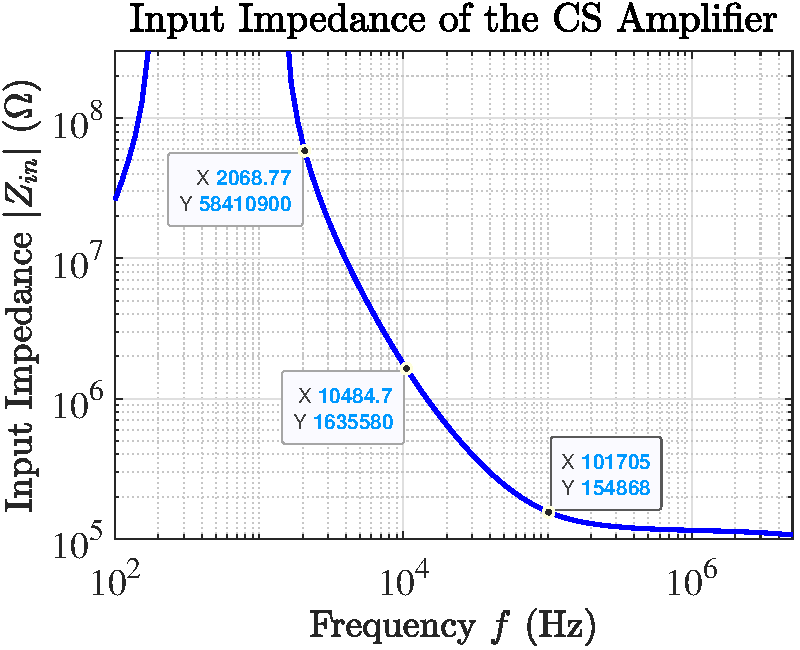
\includegraphics[width=210pt]{LCE-04-场效应管/assets/cd amp/cd Z_in.pdf}
    \hspace*{8mm}
    \caption{Input impedance curve $Z_{in} = Z_{in}(f)$}
\end{subfigure}
\caption{Common-source amp. frequency response:  at $R_S = 2.229 \ \mathrm{M}\Omega$ and the input impedance $Z_{in}$}
\end{figure}

可以看到, CD 组态的输入阻抗明显高于 CS 组态 (高了一个数量级),这主要是因为 CS 组态中寄生电容 $C_{GD}$ 由于 Miller effect 被放大了约二十倍,体现在输入端就是等效输入电容明显增大,输入阻抗降低。而 CD 组态中 $C_{GD}$ 并没有被放大,因此 CS 的输入阻抗明显小于 CD 的输入阻抗。

\subsection{CS Amp. 和 CD Amp. 的总结对比}

\begin{table}[H]\centering
    %\renewcommand{\arraystretch}{1.5} % 调整行间距为 1.5 倍
    %\setlength{\tabcolsep}{1.5mm} % 调整列间距
    \caption{Comparison between the cs amp. and the cd amp.}
    \label{table: comparison between the cs amp. and the cd amp.}
    \begin{tabular}{cccccccccc}\toprule
        Parameter & Midband gain (no load) & Input impedance & Output impedance & cut-off frequency & \\
        \midrule
        CS Amp. & 22.99 (27.23 dB) @ 100 Hz & $10.8\ \mathrm{M}\Omega\ @\ 100 \ \mathrm{Hz}$ & 1996 $\Omega$ @ 1 kHz & 372.58 kHz \\
        CD Amp. & 0.9634 (-0.324 dB) @ 100 Hz & $> 100\ \mathrm{M}\Omega\ @\ 100 \ \mathrm{Hz}$ & 33.36 $\Omega$ @ 1 kHz & > 10 MHz \\
        \bottomrule
    \end{tabular}
\end{table}

\begin{table}[H]\centering
    %\renewcommand{\arraystretch}{1.5} % 调整行间距为 1.5 倍
    %\setlength{\tabcolsep}{1.5mm} % 调整列间距
    \caption{Input impedance of the cs amp and the cd amp.}
    \label{table: input impedance of the cs amp and the cd amp.}
\begin{tabular}{cccccccccc}\toprule
    Frequency & 100 Hz & 1 kHz & 10 kHz & 100 kHz \\
    \midrule
    CS Amp. 
        & $10.8 \mathrm{M}\Omega\ @\ 100 \ \mathrm{Hz}$ 
        & $739.0 \mathrm{k}\Omega\ @\ 1 \ \mathrm{kHz}$ 
        & $53.0 \mathrm{k}\Omega\ @\ 10 \ \mathrm{kHz}$
        & $9.07 \mathrm{k}\Omega\ @\ 100 \ \mathrm{kHz}$
    \\
    CD Amp. 
        & $> 100 \mathrm{M}\Omega\ @\ 100 \ \mathrm{Hz}$
        & $> 100 \mathrm{M}\Omega\ @\ 1 \ \mathrm{kHz}$
        & $1.64 \mathrm{M}\Omega\ @\ 10 \ \mathrm{kHz}$
        & $154.9 \mathrm{k}\Omega\ @\ 100 \ \mathrm{kHz}$
    \\
    \bottomrule
\end{tabular}\end{table}

\subsection{测量 MOSFET 开关特性}

先断开全部跳线, 然后闭合跳线 J1, J4, J5, J9, 构成 CS 组态开关电路。设置输入信号为 [0 V, 5 V] 的矩形波 (1 kHz, 2.5 Vamp, 2.5 Voffset),调整示波器为 dc coupling ,得到输入输出曲线如下:
\begin{figure}[H]\centering
    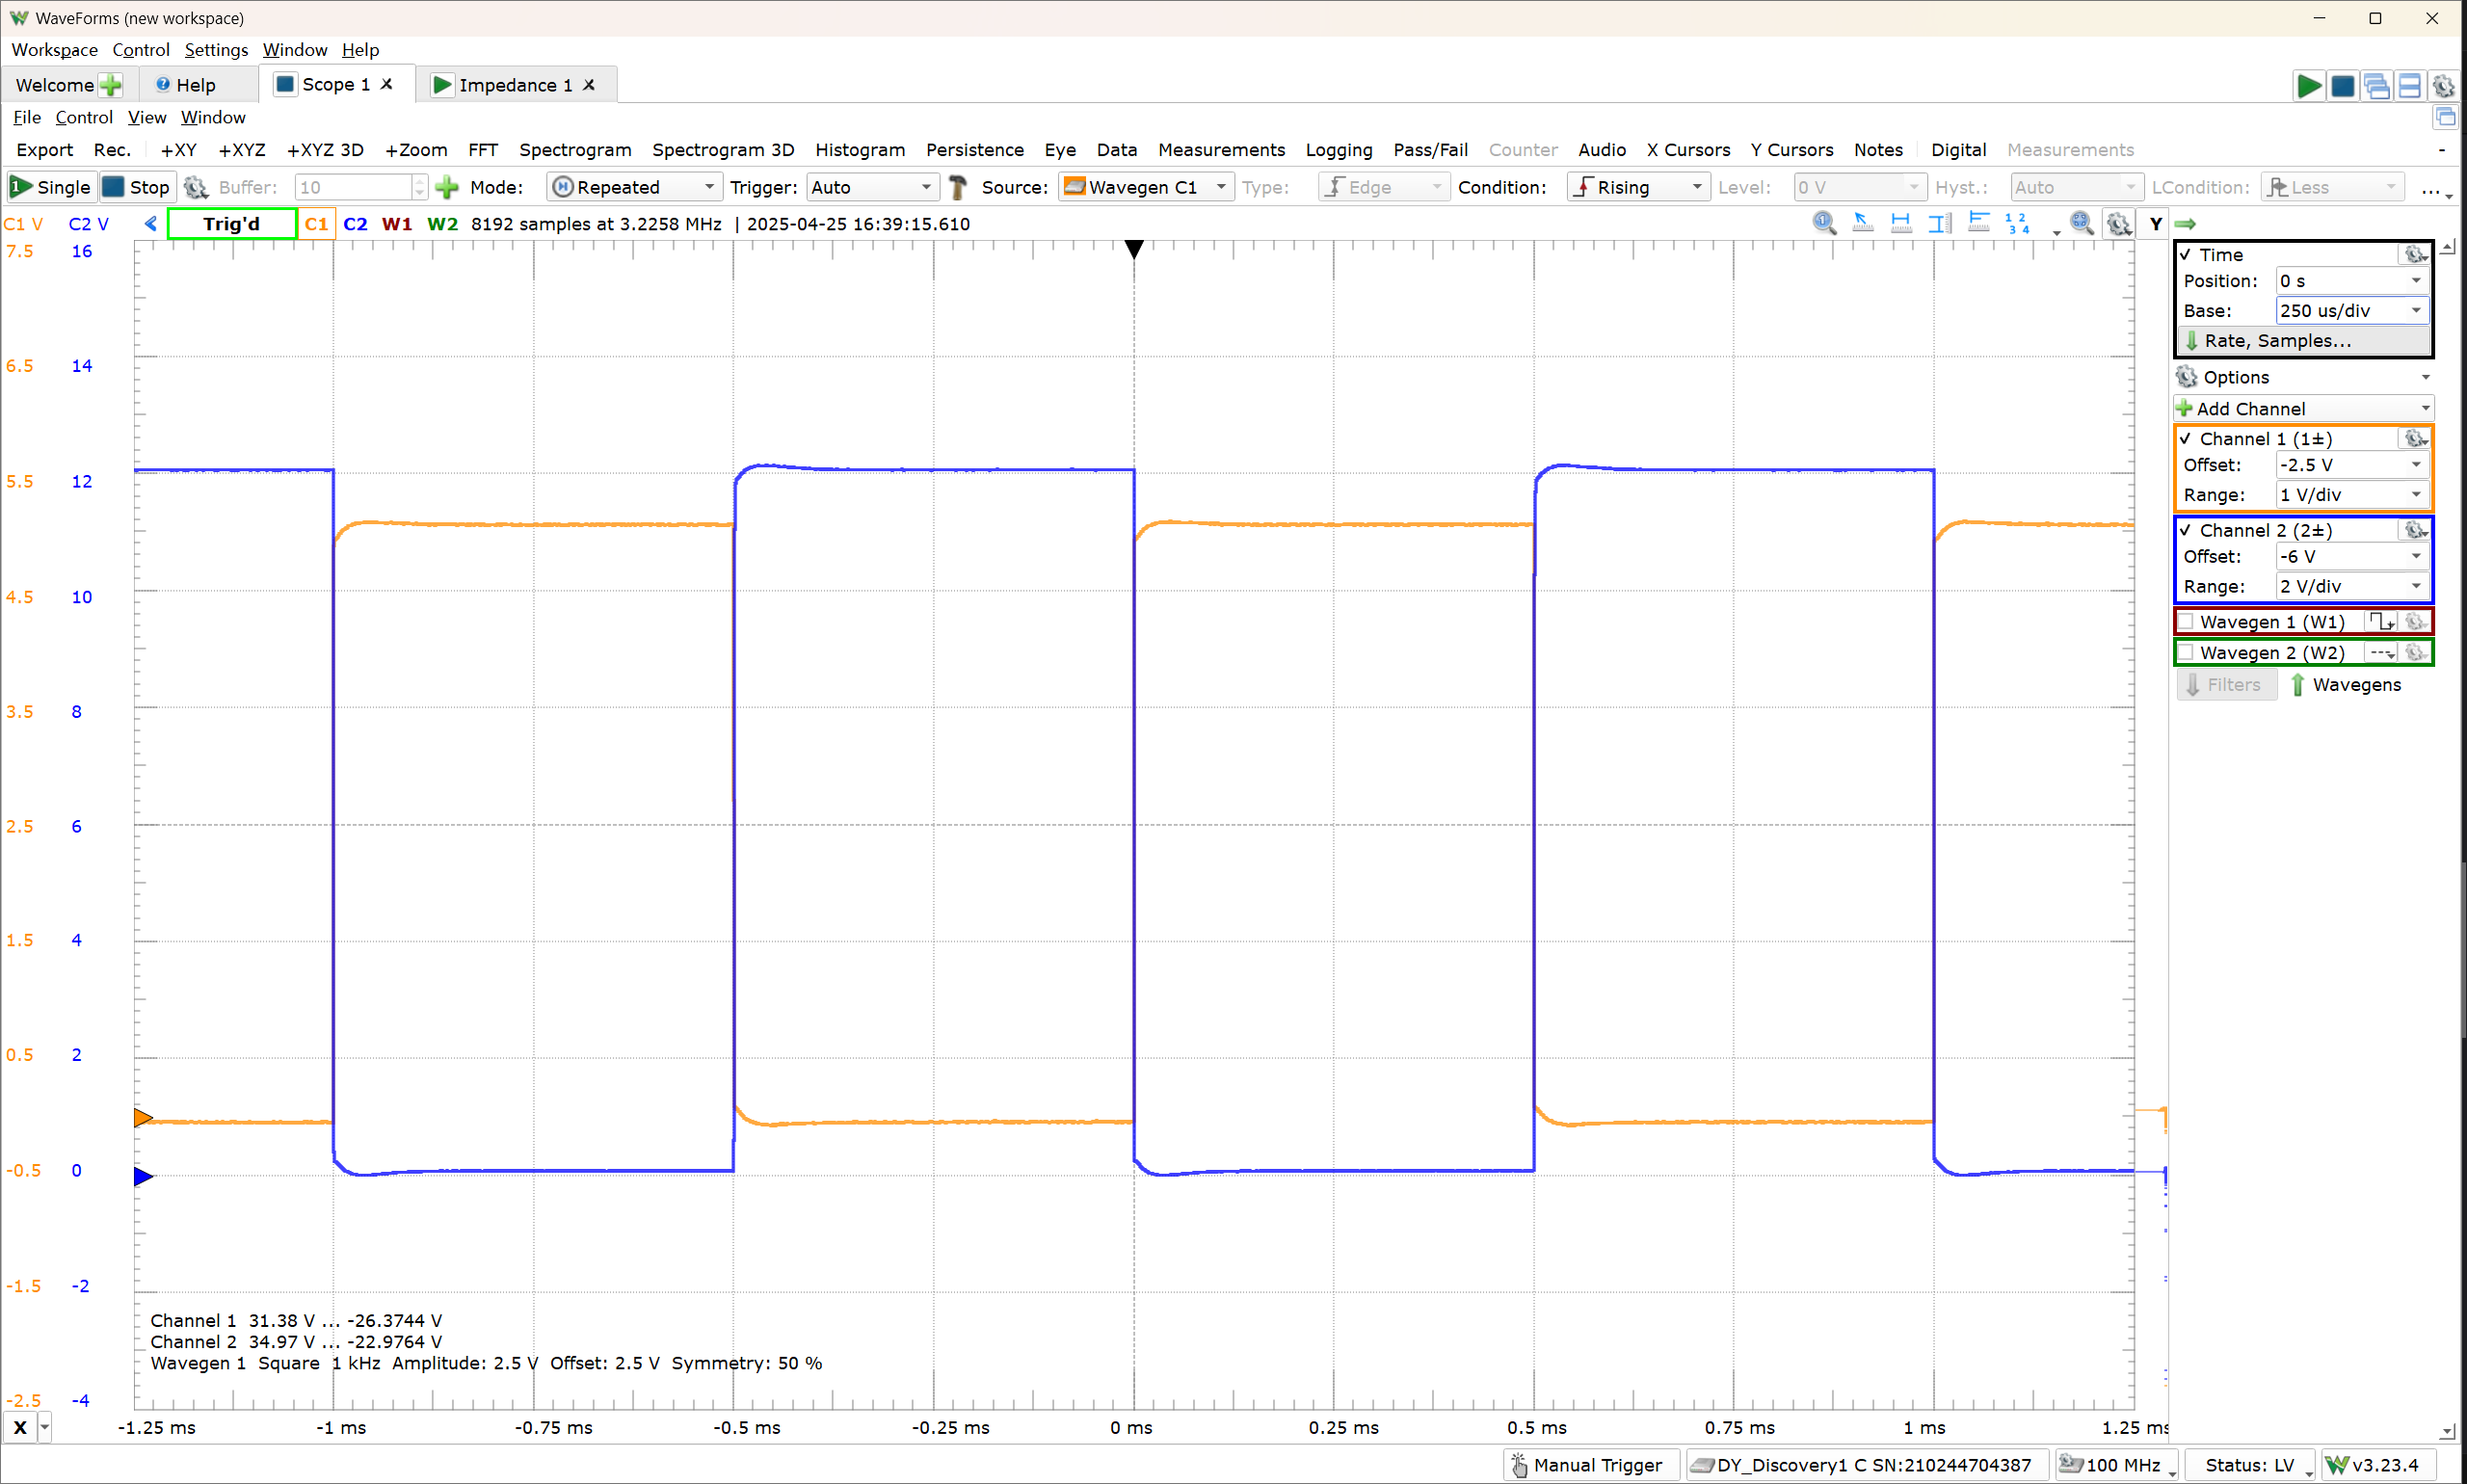
\includegraphics[width=\columnwidth]{LCE-04-场效应管/assets/switching circuit/开关 input-output 1kHz.png}
    \caption{Switching circuit I/O waveform: input signal (CH1-orange, 5 Vpp @ 1 kHz), output signal (CH2-blue), overlap display}
\end{figure}
\begin{figure}[H]\centering
    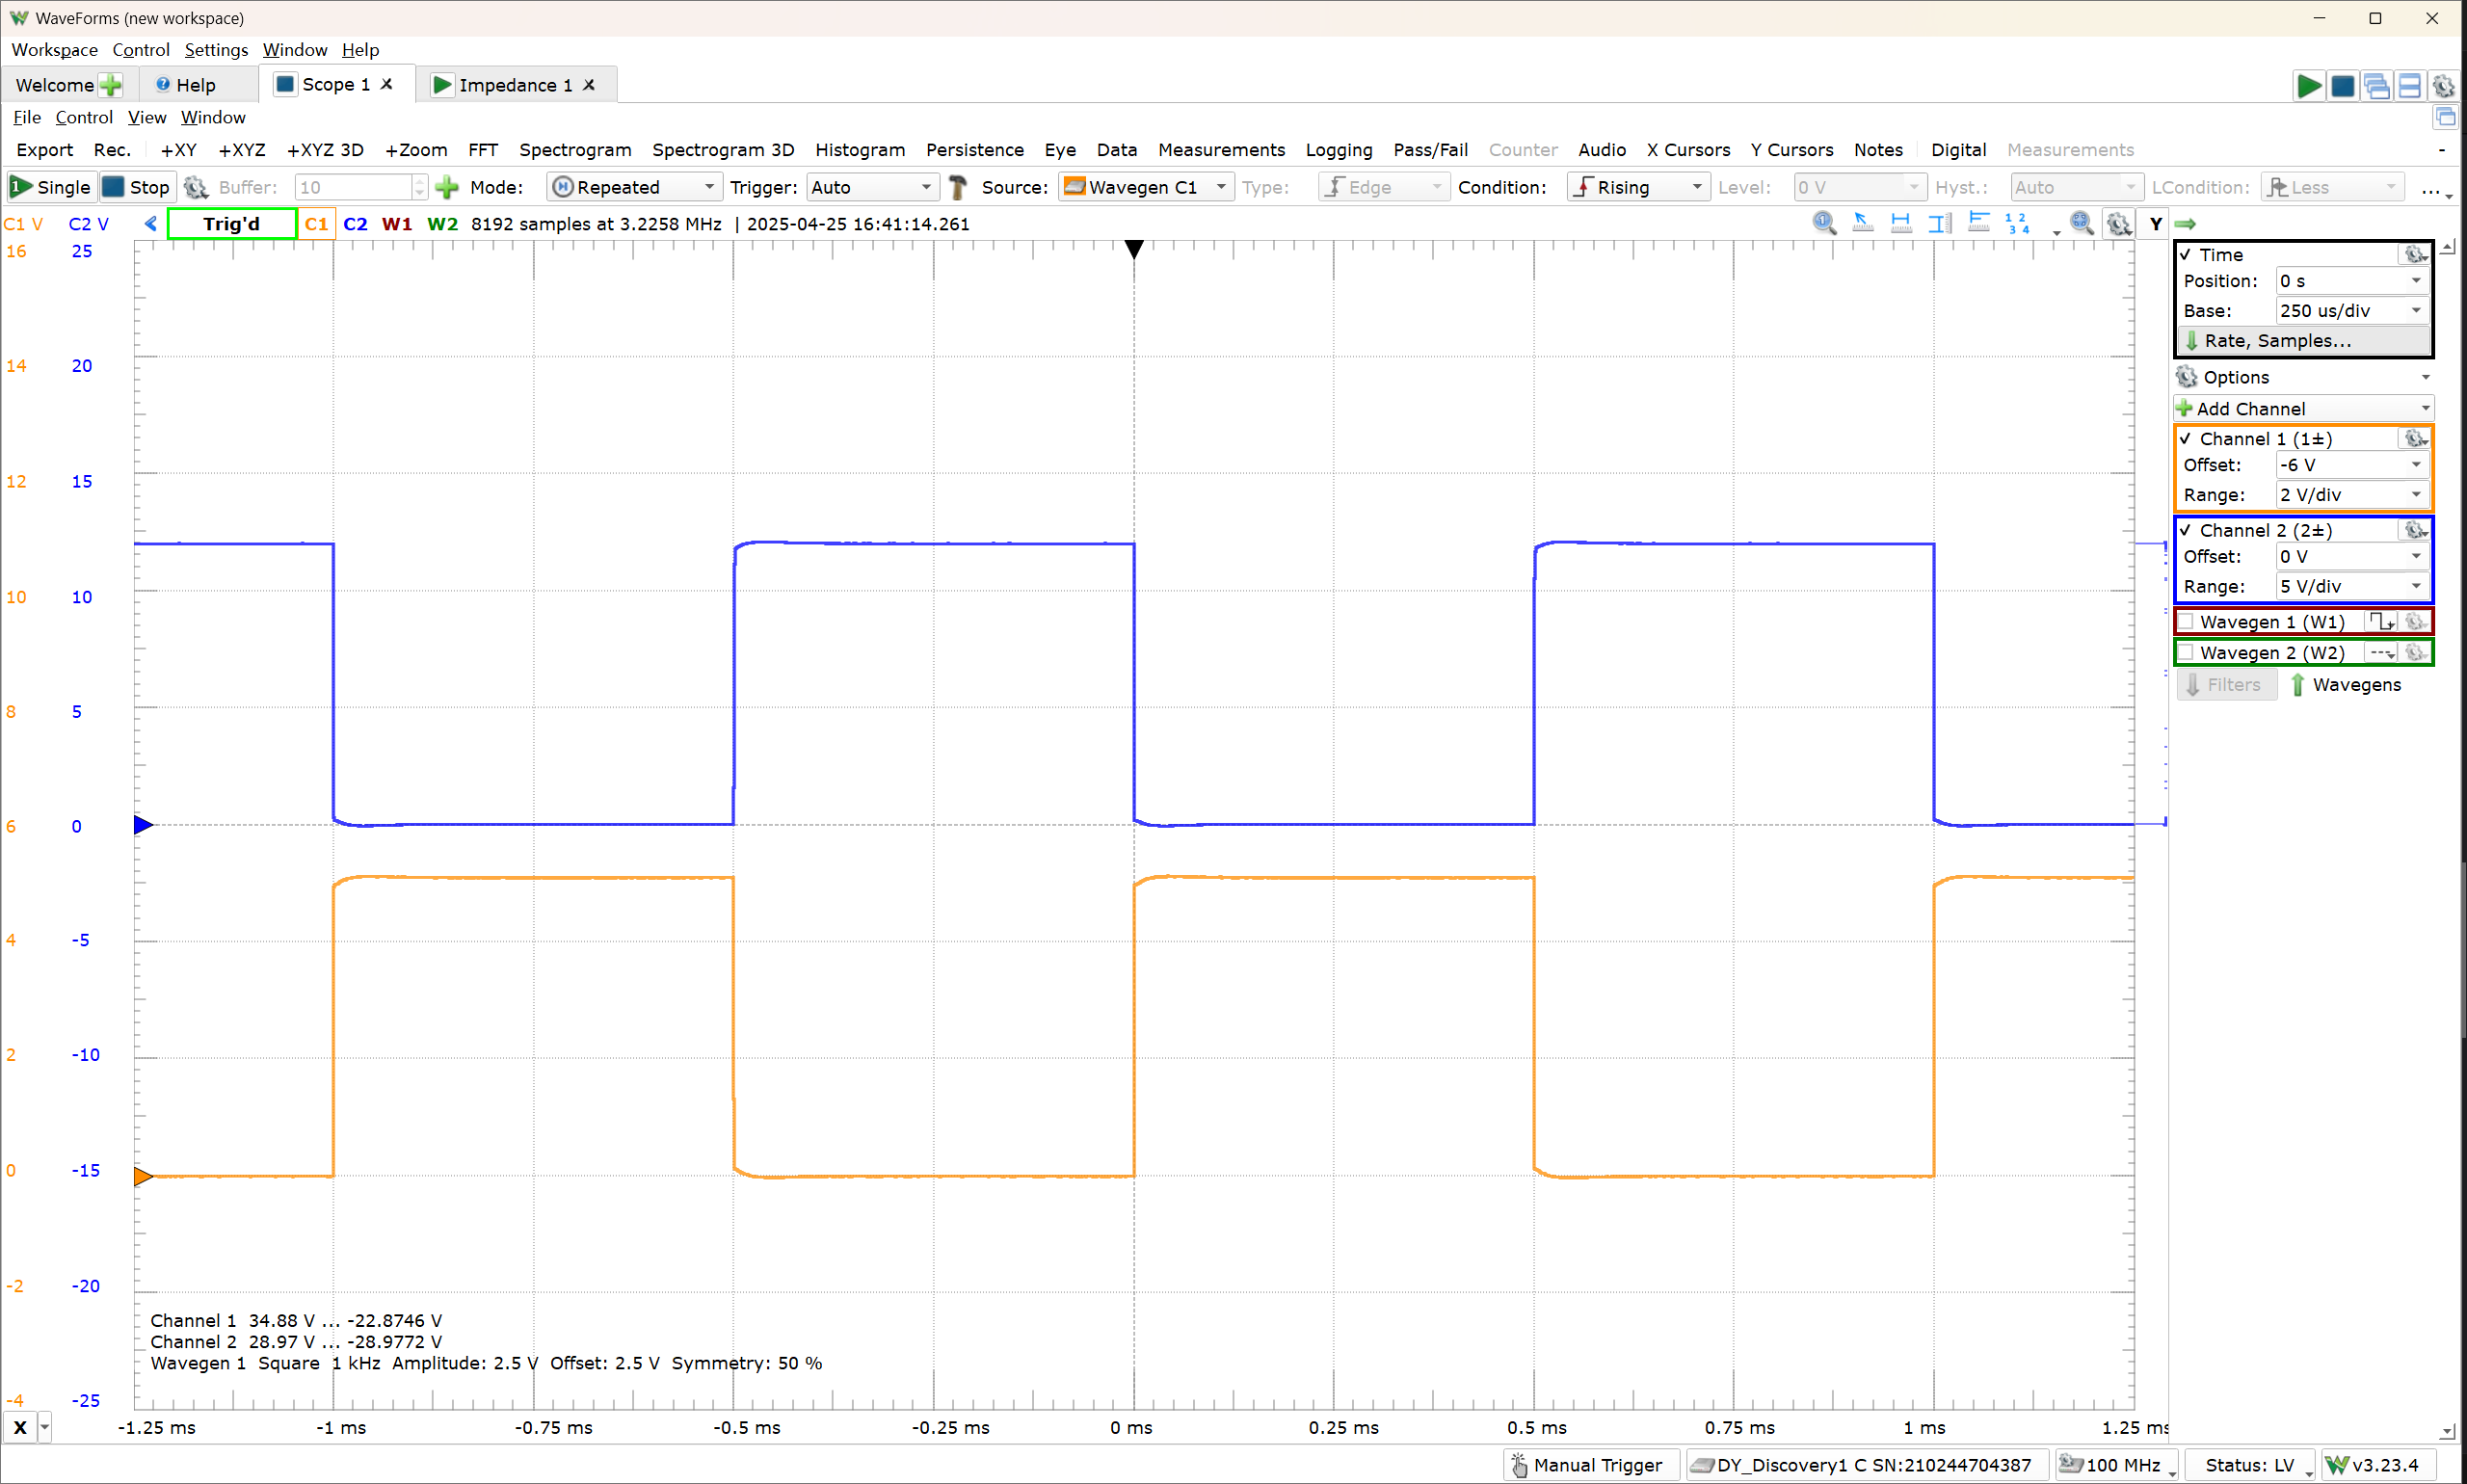
\includegraphics[width=\columnwidth]{LCE-04-场效应管/assets/switching circuit/开关 input-output (2) 1kHz.png}
    \caption{Switching circuit I/O waveform: input (CH1-orange, 5 Vpp @ 1 kHz), output (CH2-blue), misaligned display}
\end{figure}

可以看到,在 1 kHz 时开关信号是非常理想的,几乎观察不到延迟。继续调整输入信号为 100 kHz 可得:
\begin{figure}[H]\centering
    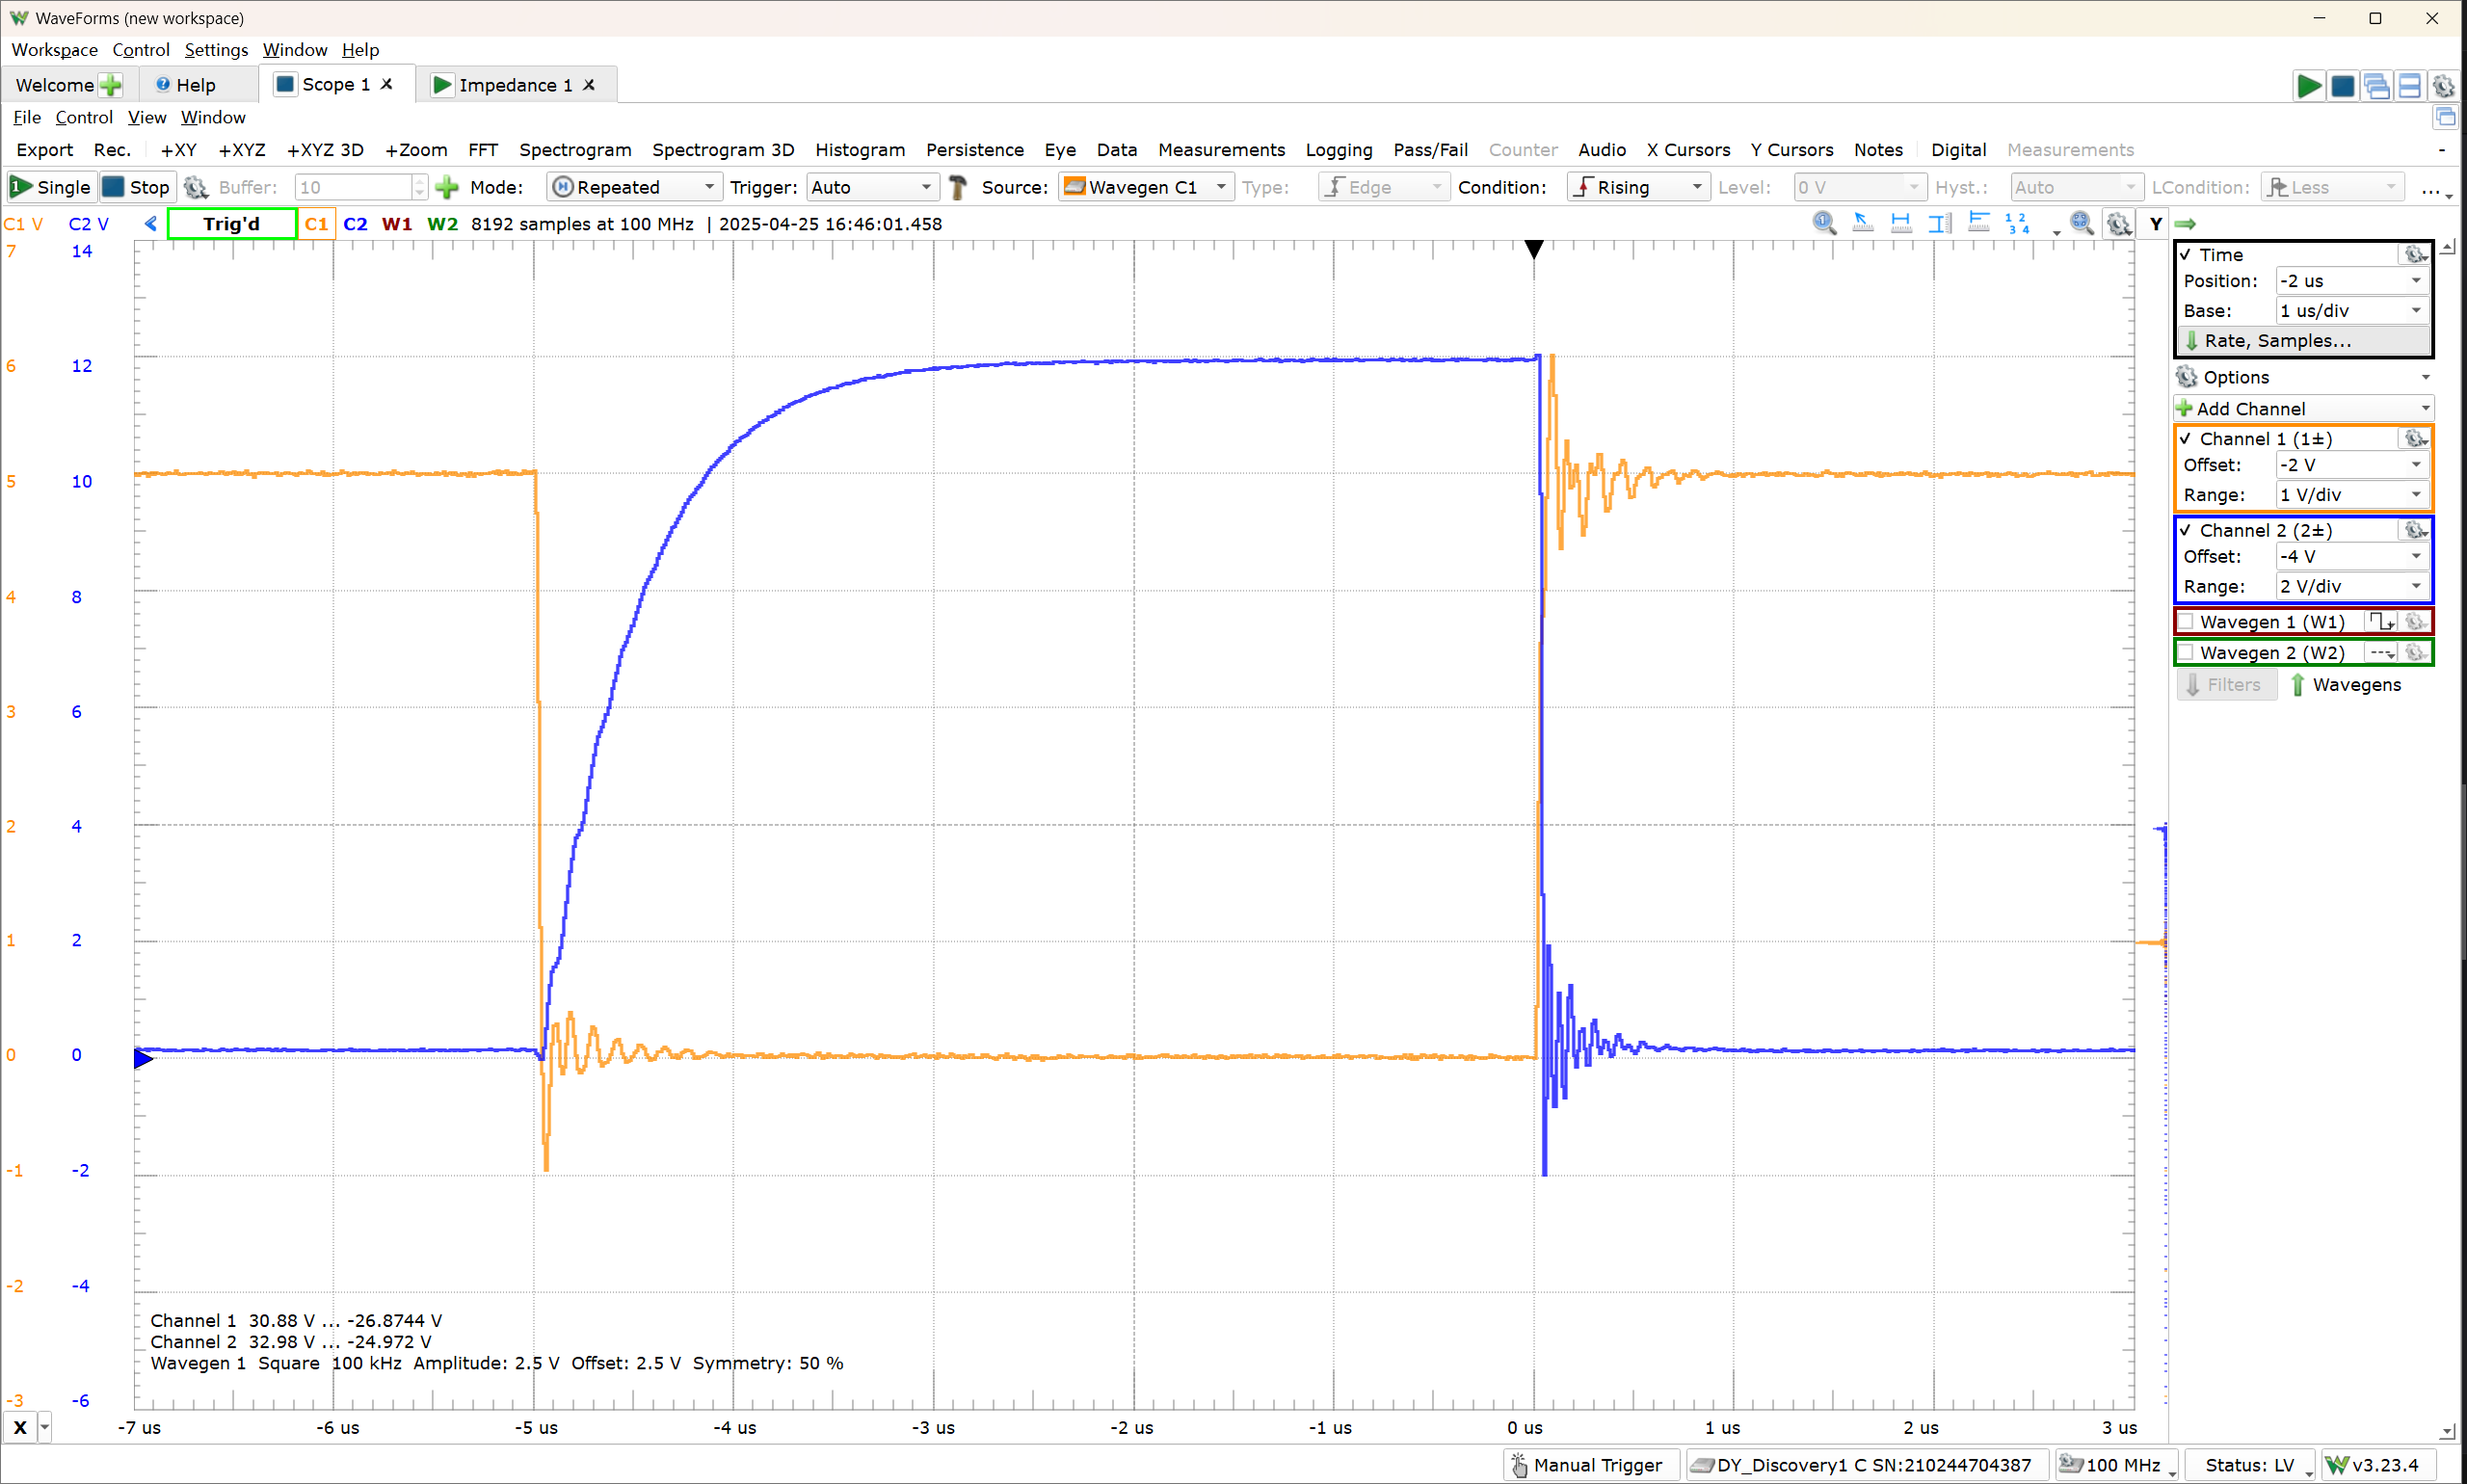
\includegraphics[width=\columnwidth]{LCE-04-场效应管/assets/switching circuit/开关 input-output 100kHz.png}
    \caption{Switching circuit I/O waveform: input (CH1-orange, 5 Vpp @ 1 kHz), output (CH2-blue), overlap display}
\end{figure}
\begin{figure}[H]\centering
    \includegraphics[width=\columnwidth]{LCE-04-场效应管/assets/switching circuit/开关 input-output 100kHz (2).png}
    \caption{Switching circuit I/O waveform: input (CH1-orange, 5 Vpp @ 1 kHz), output (CH2-blue), misaligned display}
\end{figure}

100 kHz 时,输出信号的下降沿仍比较理想,响应速度很快,但是上升沿已经有大约 800 ns 的延迟 (从 1 V 上升到 10 V)。

%\subsection{(选做) 测量 JFET (3DJ7H) 特性曲线}

\section{思考题}

\subsection{场效应管与双极性晶体管对比,有何优缺点?}

\begin{enumerate}
\item FET 集成度高: FET 工艺,尤其是 CMOS 工艺,目前已经做到非常成熟,并由此延伸出了 FinFET, GAA MOSFET 等技术。
\item FET 器件静态功耗低:一般我们认为 FET 器件是电压控制电流,而 BJT 是电流控制电流 (其实也可以视为压控器件, Razavi 在 \textit{Fundamentals of Microelectronics} 一书中便是将 BJT 也视为压控器件)。同时,考虑到 FET 的直流输入阻抗非常高 (一般在 $10^7 \ \Omega \sim 10^{12}\ \Omega$),因此一般情况下 FET 的静态功耗远低于 BJT, 后者需要不断向基极注入电流来维持工作状态。
\item FET 器件开关特性好: MOSFET 的开关特性比 BJT 好,主要是因为 FET 的输入电荷存储量远小于 BJT,无需加速电容便可以很好地开启和关断。另外,现在的大功率 MOSFET 的最大瞬时/平均电流可以做到很高 (上百安培都是很常见的),由此带来的高跨导与高开关速度使得 MOSFET 在开关电源、逆变器等应用中非常受欢迎。
\item FET 器件线性度更好: FET 器件跨导与电流的关系通常比 BJT 更为平缓,例如典型长沟道 MOSFET 的跨导 $g_m = \sqrt{2 \mu_n C_{ox} \frac{W}{L}I_D}$ 是电流的 0.5 次方,而 BJT 的跨导 $g_m = \frac{I_C}{nV_T}$ 是电流的 1 次方,因此用 FET 构建的放大器通常有更好的线性度。
\item FET 器件温漂更大: FET 器件最大的缺点之一便是较大的温漂系数,通常比同类 BJT 器件大几倍,这便要求精密 FET 电路设计必须考虑到温度补偿。
\end{enumerate} 

\subsection{本次实验的建议}

我对本次实验的建议是:考虑取消逐点法测量,并将“逐点法计算跨导”改为“导出示波器数据来计算跨导”。

我一直“偏执”地认为,任何领域、任何学科的实验,但凡使用了“逐点法”进行测量,其效率和趣味性都会大打折扣,不仅十分耗时,得到的数据质量也差强人意。本次实验的课件中要求大家用逐点法和示波器 X-Y 法测量 MOSFET 的转移特性曲线,前者的电流范围要求是 0 $\sim$ 100 mA ,并且根据此数据计算跨导 $g_m = \frac{\partial I_D }{\partial V_{GS} }$。我在上学期曾用逐点法测量过 2N7000 的转移特性曲线,整个实验过程非常繁琐,而且体验感可以说是非常糟糕。别说 0 $\sim$ 100 mA 的电流范围,我自己当时测量到 20 mA 左右,晶体管就已经出现了明显的热漂移,表现为 $V_{GS}$ 不变时 $I_D$ 缓慢增大,导致测量结果不准确。这是因为几十毫安通常达不到 zero-temperature-coefficient 点,因此 $V_{GS}$ 不变时,$I_D$ 随温度的升高而升高。而到 50 mA 左右晶体管便开始烫手 (因为已经有数百毫瓦的耗散功率了)。

因此,我建议直接用示波器的 X-Y 法测量 MOSFET 的转移特性曲线,然后将示波器数据导出,在数据处理软件中计算跨导 $g_m$。这样即提高了实验的效率,也能很大程度避免温漂问题,保证了实验结果的准确性。另一方面,数百、数千个数据计算出的跨导曲线,也比逐点法得到的跨导曲线要优越得多。也完全无需担心同学们会在数据处理上犯难,因为在上学期的“基础物理实验”一门课中,或用 Excel 或用 Origin 或用其他软件,大家早已学会了如何用相关软件去分析、处理数据。





















































\newpage
% 附录 A
\newpage
\vspace*{\fill}\begin{center}\Huge{\bfseries 
    附录 A\hspace*{20pt} 预习报告
}\end{center}\addcontentsline{toc}{section}{附录 A\hspace*{6pt} 预习报告} 
\begin{figure}[H]\centering
    \includegraphics[width=\columnwidth]{LCE-04-场效应管/assets/appendix/预习报告.png}
\end{figure}
\vspace*{\fill}
\thispagestyle{fancy} 
\includepdf[pages={-}]{LCE-04-场效应管/preview/LCE-04 (preview report).pdf}

% 附录 B
\newpage
\section*{附录 B\hspace*{20pt} 原始数据记录表}
\addcontentsline{toc}{section}{附录 B\hspace*{6pt} 原始数据记录表} 
\thispagestyle{fancy} 
\begin{figure}[H]\centering
    \includegraphics[width=0.9\columnwidth]{LCE-04-场效应管/assets/appendix/原始数据.png}
\end{figure}

% 附录
\section*{附录 C \hspace*{20pt} Matlab Codes}
\addcontentsline{toc}{section}{附录 C \hspace*{6pt} Matlab Codes} 
\thispagestyle{fancy} 
\lstinputlisting{D:/a_RemoteRepo/GH.MatlabCodes/本科课程代码/Linear Circuit Experiment/LCE_04_MOSFET.m}




\end{document}

% VScode 常用快捷键:

% F2:                       变量重命名
% Ctrl + Enter:             行中换行
% Alt + up/down:            上下移行
% 鼠标中键 + 移动:           快速多光标
% Shift + Alt + up/down:    上下复制
% Ctrl + left/right:        左右跳单词
% Ctrl + Backspace/Delete:  左右删单词    
% Shift + Delete:           删除此行
% Ctrl + J:                 打开 VScode 下栏(输出栏)
% Ctrl + B:                 打开 VScode 左栏(目录栏)
% Ctrl + `:                 打开 VScode 终端栏
% Ctrl + 0:                 定位文件
% Ctrl + Tab:               切换已打开的文件(切标签)
% Ctrl + Shift + P:         打开全局命令(设置)

% Latex 常用快捷键:

% Ctrl + Alt + J:           由代码定位到PDF


